\documentclass[12pt,final,twoside]{report}
%%%%%%%%%%%%%%%%%%%%%%%%%%%%%%%%%%%%%%%%%%%%%%%%%%%%%%%%%%%%%
% Some credits:
% The template initially was created by Prof. Dr. Holger Karl/Uni Paderborn '2006
% and was expanded and updated by Dipl.-Inform. Stefan Heinrich/Uni Paderborn/Uni Hamburg since 2008.
% Suggestions for changes are always welcome.
%%%%%%%%%%%%%%%%%%%%%%%%%%%%%%%%%%%%%%%%%%%%%%%%%%%%%%%%%%%%%
% Meta information:
\newcommand{\trtitle}{Word2Vec and Echo State Network For Thematic Role Assignment}
\newcommand{\trtype}{Master Thesis} %{Diplomarbeit} %{Dissertation}
\newcommand{\trcourseofstudies}{Intelligent Adaptive Systems} %{Bioinformatik} 
\newcommand{\trauthor}{Surender Kumar}
\newcommand{\trauthortitle}{} %{Dipl.-Inform.\ }
\newcommand{\tremail}{3kumar@informatik.uni-hamburg.de}
\newcommand{\trmatrikelnummer}{6519753}
\newcommand{\trstreet}{Kaemmererufer 13}
\newcommand{\trcity}{22303 Hamburg}
\newcommand{\trevaluatorA}{\href{mailto:wermter@informatik.uni-hamburg.de}{Prof. Dr. Stefan Wermter}}
\newcommand{\trevaluatorB}{\href{mailto:tbd@informatik.uni-hamburg.de}{ Dr. Sven Magg}}
%\newcommand{\trbetreuung}{\href{mailto:tbd@informatik.uni-hamburg.de}{Dipl.-Inform. To Be Defined}}
\newcommand{\trdepartment}{Knowledge Technology, WTM}
\newcommand{\trdate}{30.04.2013}
\newcommand{\trkeywords}{Word2Vec, ESN, Language, Semantic role labelling}

%%%%%%%%%%%%%%%%%%%%%%%%%%%%%%%%%%%%%%%%%%%%%%%%%%%%%%%%%%%%%
% Languages:
% If the thesis is written in English:
\usepackage[english]{babel}                         
\selectlanguage{english}

%%%%%%%%%%%%%%%%%%%%%%%%%%%%%%%%%%%%%%%%%%%%%%%%%%%%%%%%%%%%%
% Bind packages:
\usepackage{acronym}                    % Acronyms
\usepackage{algorithmic}                % Algorithms and Pseudocode
\usepackage{algorithm}                  % Algorithms and Pseudocode
\usepackage{amsfonts}                   % AMS Math Packet (Fonts)
\usepackage{amsmath}                    % AMS Math Packet
\usepackage{amssymb}                    % Additional mathematical symbols
\usepackage{amsthm}
\usepackage{booktabs}                   % Nicer tables
%\usepackage[font=small,labelfont=bf]{caption} % Numbered captions for figures
\usepackage{color}                      % Enables defining of colours via \definecolor
\definecolor{uhhRed}{RGB}{226,0,26}     % Official Uni Hamburg Red
\definecolor{uhhGrey}{RGB}{136,136,136} % Official Uni Hamburg Grey
\definecolor{uhhLightGrey}{RGB}{220, 220, 220}
\usepackage{fancybox}                   % Put equations in a frame
\usepackage{fancyhdr}                   % Packet for nicer headers
%\usepackage{fancyheadings}             % Nicer numbering of headlines
\usepackage[body={5.8in,9in}]{geometry} % Type area (size, margins...)
\usepackage{enumitem}

%\geometry{a4paper,outer=3.35cm}        % !!!Release version (Normal margins)
%\geometry{a4paper,outer=2.5cm}         % !!!Print version (Additional margin on the left for the binding)
%\geometry{a4paper}                     % !!!Proofread version (Additional margin on the right for corrections)
\geometry{a4paper,outer=3.15cm}         % !!!Draft version (Same margins on left and right)
%\geometry{paperheight=10.0in,paperwidth=6.4in,top=0.51in,left=0.3in}  % !!!Developer version (Minimal margins)

\usepackage{graphicx}                   % Inclusion of graphics
\usepackage{latexsym}                   % Special symbols
\usepackage{longtable}                  % Allow tables over several parges
\usepackage{listings}                   % Nicer source code listings
\usepackage{multicol}                   % Content of a table over several columns
\usepackage{multirow}                   % Content of a table over several rows
\usepackage{rotating}                   % Alows to rotate text and objects
\usepackage[hang]{subfigure}            % Allows to use multiple (partial) figures in a fig
%HINT: subfigure may be outdated already - maybe try subfig instead 
%\usepackage[font=footnotesize,labelfont=rm]{subfig}    % Pictures in a floating environment
\usepackage{tabularx}                   % Tables with fixed width but variable rows
\usepackage{url,xspace,boxedminipage}   % Accurate display of URLs
\usepackage[table,xcdraw]{xcolor}
\usepackage{booktabs,caption,fixltx2e}
\usepackage[flushleft]{threeparttable}
%%%%%%%%%%%%%%%%%%%%%%%%%%%%%%%%%%%%%%%%%%%%%%%%%%%%%%%%%%%%%
% PDF Information und Definitions:
\author{\trauthor}

\ifx\pdftexversion\undefined
\usepackage{hyperref}
\else
\usepackage[colorlinks=false,           % link is colores (true) or has colored frame (false)
            linkcolor=uhhRed,           % case colorlinks=true: define color.
            urlcolor=uhhRed,
            citecolor=uhhRed,
            bookmarks,                  % Place bookmarks erstellen
            bookmarksopen=true,         % Bookmarks will be shown at start (true/false)
            pdfpagemode=UseOutlines,    
            bookmarksopenlevel=1,       % Define the depth of shown links
            bookmarksnumbered,          % Numbers of chapers in Bookmarks
            pdftitle={\trtitle},
            pdfsubject={\trtype},
            pdfkeywords={\trkeywords},
            pdfauthor={\trauthor},
            plainpages=false
            ]{hyperref}
\fi

\ifx\pdftexversion\undefined
\else
\pdfoutput=1                            % Disable PDF-Output
\pdfimageresolution=1200
\pdfcompresslevel=2                     % 0 = no compression, 9 = strongest compression
\fi

%%%%%%%%%%%%%%%%%%%%%%%%%%%%%%%%%%%%%%%%%%%%%%%%%%%%%%%%%%%%%
% Configurationen:

\hyphenation{whe-ther}                  % Manually use: "\-" in a word: Staats\-ver\-trag
\numberwithin{equation}{section}
%\lstloadlanguages{C}                   % Set the default language for listings
\DeclareGraphicsExtensions{.pdf,.svg,.jpg,.png,.eps} % first try pdf, then eps, png and jpg
\graphicspath{{./src/}}                 % Path to a folder where all pictures are located
\pagestyle{fancy}                       % Use nicer header and footer

% Redefine the environments for floating objects:
\setcounter{topnumber}{3}
\setcounter{bottomnumber}{2}
\setcounter{totalnumber}{4}
\renewcommand{\topfraction}{0.9}        %Standard: 0.7
\renewcommand{\bottomfraction}{0.5}     %Standard: 0.3
\renewcommand{\textfraction}{0.1}       %Standard: 0.2
\renewcommand{\floatpagefraction}{0.8}  %Standard: 0.5

% Tables with a nicer padding:
\renewcommand{\arraystretch}{1.2}

% Chapter and Sections will not be written in capitals
\renewcommand{\chaptermark}[1]{\markboth{\chaptername \ \thechapter.\ #1}{}}
\renewcommand{\sectionmark}[1]{\markright{\thesection.\ #1}}

%%%%%%%%%%%%%%%%%%%%%%%%%%%%
% Additional 'theorem' and 'definition' blocks:
\theoremstyle{plain}
\newtheorem{theorem}{Theorem}[chapter]
%\newtheorem{theorem}{Satz}[chapter]    % Wenn in Deutsch geschrieben wird.
\newtheorem{axiom}{Axiom}[chapter]     
%\newtheorem{axiom}{Fakt}[chapter]      % Wenn in Deutsch geschrieben wird.
%Usage:%\begin{axiom}[optional description]%Main part%\end{fakt}

\theoremstyle{definition}
\newtheorem{definition}{Definition}[chapter]

%Additional types of axioms:
\newtheorem{lemma}[axiom]{Lemma}
\newtheorem{observation}[axiom]{Observation}

%Additional types of definitions:
\theoremstyle{remark}
%\newtheorem{remark}[definition]{Bemerkung} % Wenn in Deutsch geschrieben wird.
\newtheorem{remark}[definition]{Remark} 

%%%%%%%%%%%%%%%%%%%%%%%%%%%%
% Provides TODOs within the margin:
\newcommand{\TODO}[1]{\marginpar{\emph{\small{{\bf TODO: } #1}}}}

%%%%%%%%%%%%%%%%%%%%%%%%%%%%
% Abbreviations and mathematical symbols
\newcommand{\modd}{\text{ mod }}
\newcommand{\RS}{\mathbb{R}}
\newcommand{\NS}{\mathbb{N}}
\newcommand{\ZS}{\mathbb{Z}}
\newcommand{\dnormal}{\mathit{N}}
\newcommand{\duniform}{\mathit{U}}

\newcommand{\erdos}{Erd\H{o}s}
\newcommand{\renyi}{-R\'{e}nyi}
% it is recommented to define complex terms as expression/newcommand and use the expression in the tex instead.

%%%%%%%%%%%%%%%%%%%%%%%%%%%%%%%%%%%%%%%%%%%%%%%%%%%%%%%%%%%%%
% Document:

\begin{document}

\pagenumbering{Roman}                   % Roman pagenumbering for lists and meta pages
\renewcommand{\headheight}{14.5pt}      % Size of headings

\thispagestyle{empty}
\fancyhead[LO,RE]{}                     % Define the header style for the meta pages

%%%%%%%%%%%%%%%%%%%%%%%%%%%%
% Cover sheet

\begin{titlepage}
%---Possibility 1:
    \begin{flushleft}
        
\includegraphics[width=85mm]{uhhLogoL.pdf}\\
    \end{flushleft}
%---Possibility 2:
%\includegraphics*[width=0.09\textwidth]{uhhIconR_}
%\parbox[c]{10cm}{
%    \begin{center}
%    Universit\"at Hamburg --- MIN-Fakult\"at\\
%    \trfachgruppe
%    \end{center}
%    }\hfill
%\includegraphics*[width=0.09\textwidth]{infIcon_}
%\vspace{0.2cm}
%---
    \rule{\textwidth}{0.4pt}
        \newline
        \vspace{2.0cm}
        \begin{center}
          \LARGE \textbf{\trtitle}
        \end{center}
    \vspace{2.0cm}
    \begin{center}
      \textbf{\trtype}\\
      %am Fachgebiet \trdepartment\\
      at the Research Group \trdepartment\\
      \trevaluatorA\medskip\\
      Department Informatik\\
      MIN-Fakult\"at\\
      Universit\"at Hamburg \\[0.5cm]
      Submitted by \\
      \textbf{\trauthortitle\href{mailto:\tremail}{\trauthor}}\\
      on\\
      \trdate
    \end{center}
    \vspace{1cm}
    \begin{center}
    \begin{tabular}{ll}
    Evaluators: & \trevaluatorA \\
                   & \trevaluatorB \\
    %Betreuung: & \trbetreuung \\    	% Adviser are not allowed to demand getting credited, but are happy getting credited by the students initiative
    \end{tabular}
    \end{center}
    \vfill
    \begin{tabular}{l}
    \trauthor \\
    Matriculation Number:  \trmatrikelnummer \\
    \trstreet \\
    \trcity
    \end{tabular}
    \newline
    \rule{\textwidth}{0.4pt}
    \newpage 
\end{titlepage}

    %backsite of cover sheet is empty!
\thispagestyle{empty}
\hspace{1cm}
\newpage

%%%%%%%%%%%%%%%%%%%%%%%%%%%%
% Abstract:
\section*{Abstract}\label{sec:abstract}
%\fancyhead[LE,RO]{\it Abstract}
%\addcontentsline{toc}{chapter}{\numberline{}Abstract}
Humans have a remarkable capability of acquiring language and in particular more than one languages. More interestingly they learn it within the same neural computing substrate. But how does the structure of a sentence is mapped to its meaning within the brain is still an open issue?  



% If the abstract ist not longer than half a page, then the German Zusammenfassung can be places on the same page
%\cleardoublepage
\vfill
\section*{Zusammenfassung}\label{sec:zusammenfassung}
%\addcontentsline{toc}{chapter}{\numberline{}Zusammenfassung} %Add the Zusammenfassung to the TOC
Hier die deutsche Zusammenfassung einf\"ugen (notwendig).
\fancyhead[LE,RO]{\it Abstract}

\cleardoublepage

%%%%%%%%%%%%%%%%%%%%%%%%%%%%
% Lists:
%\setcounter{tocdepth}{1}               % depth of the table of contents (for BSc and MSc Thesis 1 is recommented)
\fancyhead[LE,RO]{\it Contents}
\tableofcontents
\cleardoublepage
% List of Figures and List of tables are optional. -> Not needed in most theses.
\fancyhead[LE,RO]{\it List of Figures}
\listoffigures
\cleardoublepage
\fancyhead[LE,RO]{\it List of Tables}
\listoftables
\cleardoublepage
%\lstlistoflistings
%\cleardoublepage

\fancyhead[LE]{\it \leftmark}           % Define the header style for the text pages
\fancyhead[RO]{\it \rightmark}          % Define the header style for the text pages
\fancyhead[LO,RE]{}                     % Define the header style for the text pages

%%%%%%%%%%%%%%%%%%%%%%%%%%%%
% The content will be included here:
\pagenumbering{arabic}

\chapter{Introduction}\label{introduction}

Thematic Role Assignment (TRA) is a supervised learning problem which aims to identify events and its participants from a sentence and determine \textit{"Who did what to whom"}. In other words assigning roles to words (arguments) in a sentence with respect to a verb (predicate). The role typically includes agent, object, recipient etc.. For example in the sentence \textit{"the dog that gave the rat to the cat was hit by the man"}, the first noun \textit{'dog'} is the agent of verb \textit{'gave'} and object of verb \textit{'hit'}. In Natural Language Processing terminology (NLP) the problem is studied under the name of Semantic Role Labelling (SRL). Hence, TRA or SRL is a form of simplistic semantic parsing which aims to determine the predicate-argument structure for a verb in the given sentence \cite{end-to-end}. Understanding the semantics of the text plays an important intermediate step in a wide range of real-world applications such as machine translation \cite{srl:machine_translation}, information extraction \cite{srl:info_extraction:hri}, sentiment analysis \cite{srl:sentiment:wang}, document categorization \cite{srl:text_categorization:persson}, human robot interaction \cite{tra:xavier_hri,srl:info_extraction:hri} etc.

\section{Previous Work}

Many successful traditional system consider SRL as a multiclass classification problem use linear classifier such as Support Vector Machines (SVM) to tackle the problem \cite{Koomen:2005,srl:pradhan:2004,pradhan:2005}. These system were based on pre-defined feature templates derived from syntactic information obtained by parsing and producing parse trees of the sentences in the training corpus. However in an analysis it was found that the use of syntatic parser certainly leads to degradation of predictions \cite{pradhan:2005}. Also  designing of feature templates need a lot of heuristics and time. The pre-defined features are often required to be iteratively modified depending on how the system perfoms. The feature templates are often required to be re-desinged when the task is to be performed on different languages, corpus or when the data distribution is changed \cite{end-to-end}.

In order to avoid engineering manual feauture templates, SRL task was also attempted with neural network models. Collobert et al. \cite{srl:collobert:2011} first attempted to build an end-to-end system without parsing by using word embeddings and Convolutional Neural Network (CNN). The model was less successful as CNN cannot employs long term dependencies within a sentence since it can only take into account the words in limitied context \cite{end-to-end}. However to increase the model perfomance they also resorted to use syntatic features by using parse trees of charnink parser \cite{charniak_parser:2000}.

% TODO: Improve it
Recurrent Neural Networks (RNN) has been also been used for wide range NLP task and also recently with Echo State Network (ESN): a varinat of RNN. The tasks used were diverse from perdicting next word given the previous words to learning grammatical structures \cite{esn:learn_gs}.  RNN makes use of sequential information and acts as a memory unit and captures the information processed in the past \cite{rnn:elman:1990}. The ESN have several advantages over simple RNN. First, ESNs are capable of modeling long term dependencies in the sentence. Second, while processing long sequence the gradient parameter vanishes or explodes in simple RNNs \cite{rnn:gradiant_problem:bengio}. Third, unlike simple RNN ESNs are computationally cheap as in ESN the recurrent layer (reservoir) is randomly initialized and only connections from recurrent layer to read-out layers are learned \cite{esn:NIPS:2003, esn:practical_guide}. These advantages of ESN over RNN makes it good choice to be used for TRA task.

Xavier et al. \cite{xavier:2013:RT} proposed a generic neural network architecture using Recurrent Neural Network based on reservoir computing approaches, namely Echo State Network to solve TRA task. The proposed architecture models the language acquisition in brain and provided a robust and scalable implementation on robotics architecture \cite{xavier:2013:RT,tra:xavier_hri}. They called this model as $\theta RARes$. The model is based on the notion of grammatical construction: mapping of word order (surface form) to its meaning. They first transformed the raw sentences by replacing the semantic words (nouns, verbs etc.) with a unique token $'SW'$ then the sentences are input to model sequentially, word by word across time along with the coded meaning (i.e. thematic roles of semantic words) of the input sentence for training. The model learns the thematic roles of all the semantic words in the input sentence during training. During testing, the model predicts the coded meaning of the previously unseen sentences. See chapter \ref{issues} for more details about $\theta RARes$ model.

\section{Motivation and Hypothesis}

Like many other traditional NLP system they also treated words as discrete atomic symbols and used localist vector respresentaion of words as an input. Treating each word as a dicrete symbol does not provide any relational information to the model which may exist between two words. For example, if words \textit{'pink'} and \textit{'red'} are represented using localist representation with vectors [1,0] and [0,1] respectively, then the semantic relationship (i.e. both are colors) between these two words is lost \cite{w2v:tensor_flow}. Although, replacing the semantic words with $'SW'$ token makes it possible to train the model on a small corpus as the $'SW'$ token can be replaced with different semantic words (nouns, verbs etc.) to form a sentence. Whereas on the other hand the 'SW' token in iteself does not carry any semantics and thus does not allow model to take into account the semantics of the words. This makes it difficult for the model to learn thematic roles for sentences. We discuss more in detail about the limitation of this model later in Chapter \ref{issues}.

Motivated by the limitations of localist input representation of words and transformation of raw sentences into its abstract form by replacing semantic words with 'SW' token described above, we hypothesize that the use of distributed word representation which can capture the syntactic and semantic relationship of words could possibly improve the perfomance of the model on TRA task. One such model for learning distributed word vectors was proposed by Mikolov et al. \cite{w2v:mikolov_2013_distributed} widely known as Word2Vec model. Word2Vec model learn high quality, low-dimensional vector represenation of words from a large corpus in an unsupervised way[ref-two]. The resulting word vector of this model encodes semantics of words. As the model learns the embeddings by taking into account the context words, the obtained vector embeddings also encodes several language regularities and patterns[ref] and can be observed by performing linear operation on the word vector. For example, \textit{vector('king') - vector('man') + vector('woman') $\approx$ vector('queen')}. Unlike other neural network models for obtaining word embeddings, training Word2Vec is computationally cheap and efficient[ref?]. Training of word2vec model and properties of resulting distributed word embedding will be discussed in detail in Chapter \ref{basics}. 

\section{Proposed Models}

In this work, we thus propose a end-to-end system called \textit{Word2Vec-ESN} model, for TRA task. The Word2Vec-ESN model is a combination of word2vec model and ESN. The word2vec model is trained on a general purpose unlabelled dataset (e.g. wikipedia) prior to use of model for TRA task. The word2vec unit being the first unit, receives the raw sentences and generates the distributed word embeddings of the constituent words. The generated word vector by word2vec model can then be used by ESN for learning thematic roles of the input sentences. Note that the proposed model is basically a modified verision of $\theta RARes$ model \cite{xavier:2013:RT}, where unlike the latter raw sentences are not transformed to grammatical construcion and word2vec word vectors are used over localist word representation as an input to ESN. 

Apart from Word2Vec-ESN model, we also propose a variant of this model which only differs from the original in the way the sentences are processed and results are evaluated. Thus in this model variant the inputs and outputs of the model are changed. The input feautre to this model variant is the current word and the verb with respect to which it is processed. The output units encodes the possible role (e.g. predicate, agent, object, recipient and No Role) of the input words unlike the original model where output units encodes the thematic roles of all sematic words in the input sentence. For the evaluation of this model variant we used metrics (classification scores) proposed for CoNLL-2005 SRL task[ref]. Both Word2Vec-ESN model and its variant is discussed in mored detail in chapter \ref{approach}.

[TODO:Describe the overview of results here.]

\section{Scope of work}

There are several other ways of obtaining word embeddings [glove and other] but a systematic comparision of them on TRA task is beyond the scope of this work. Using word2vec model, distributed word vectors of different dimesions can be obtained and used for TRA task. Evaluating and comparing the effect of dimesnsion of these word embedding is also not the focus of this study. To this date, there is no research conducted with this combination of word2vec model and ESN. This also makes this study novel.

\section{Outline}

In the next chapter we give a description of  word2vec model and echo state network model. We also descibe in detail the training of word2vec model and properties of word2vec word vectors. Alse this chapter describes training and control parameters of ESN. The chapter \ref{issues} describes the  $\theta RARes$ model, its limitations and the motivation and hypothesis for the current work. Subsequently in chapter \ref{approach} we propose the Word2Vec-ESN model and its variant. This chapter also describes the data, implementation and evaluation metrics used in our experiments. Chapter \ref{results} contains the experiments and results performed for TRA task with proposed model along with the results. This chapter we also compares the results of Word2Vec-ESN model with the results obtained from  $\theta RARes$ model and analysis them. Finally, in the chapter \ref{conclusion} we describe the conclusion of this study and the possible future work.








\cleardoublepage

\chapter{Basics of Word2Vec and Echo State Network}\label{basics}

\section{Word2Vec}

Word2vec is a neural probalistic language model based on Distributional Hypothesis which states that the words that appears in the same context share the semantic meaning \cite{w2v:tensor_flow}. The proposed by Mikolov et al. \cite{w2v:mikolov_2013_distributed}, which takes in input a large text data to generate the distributed word  embedding of the words present in text and also preserve the linear regularities among words. In other words, it maps the words into a continuous vector space where semantically related words are placed closed to each other in the vector space. Earlier the words have been treated as discrete atomic symbols in all traditional NLP system, where each word were represented in a localist fashion. Localist representation of words does not contain any semantic or syntactic information of the word it is encoding and thus depriving the NLP systems to utilize this information while processing \cite{w2v:baroni:2014}. Word2vec neural word embeddings overcomes this issue and capture the semantics and syntactic information of the word in a computationally-efficient manner \cite{w2v:mikolov_2013_efficient}. For learning word embedding two neural architecture were proposed, the Continuous Bag Of Word (CBOW) and Skip-Gram (SG) \cite{w2v:mikolov_2013_efficient, w2v:mikolov_2013_distributed}. Both the models are architecturally same i.e. both have three layers, the input layer, hidden layer and an output layer, but have different training objectives. The architecture of both CBOW and SG models is shown in figure \ref{fig:cbow} and \ref{fig:sg} respectively. In the next sections we give a brief overview of CBOW model and SG model. However we used skip-gram model in our work because it was proven that it produce better word-embeddings as compared to CBOW \cite{w2v:mikolov_2013_distributed}.

\begin{figure}[hbtp]
\centering
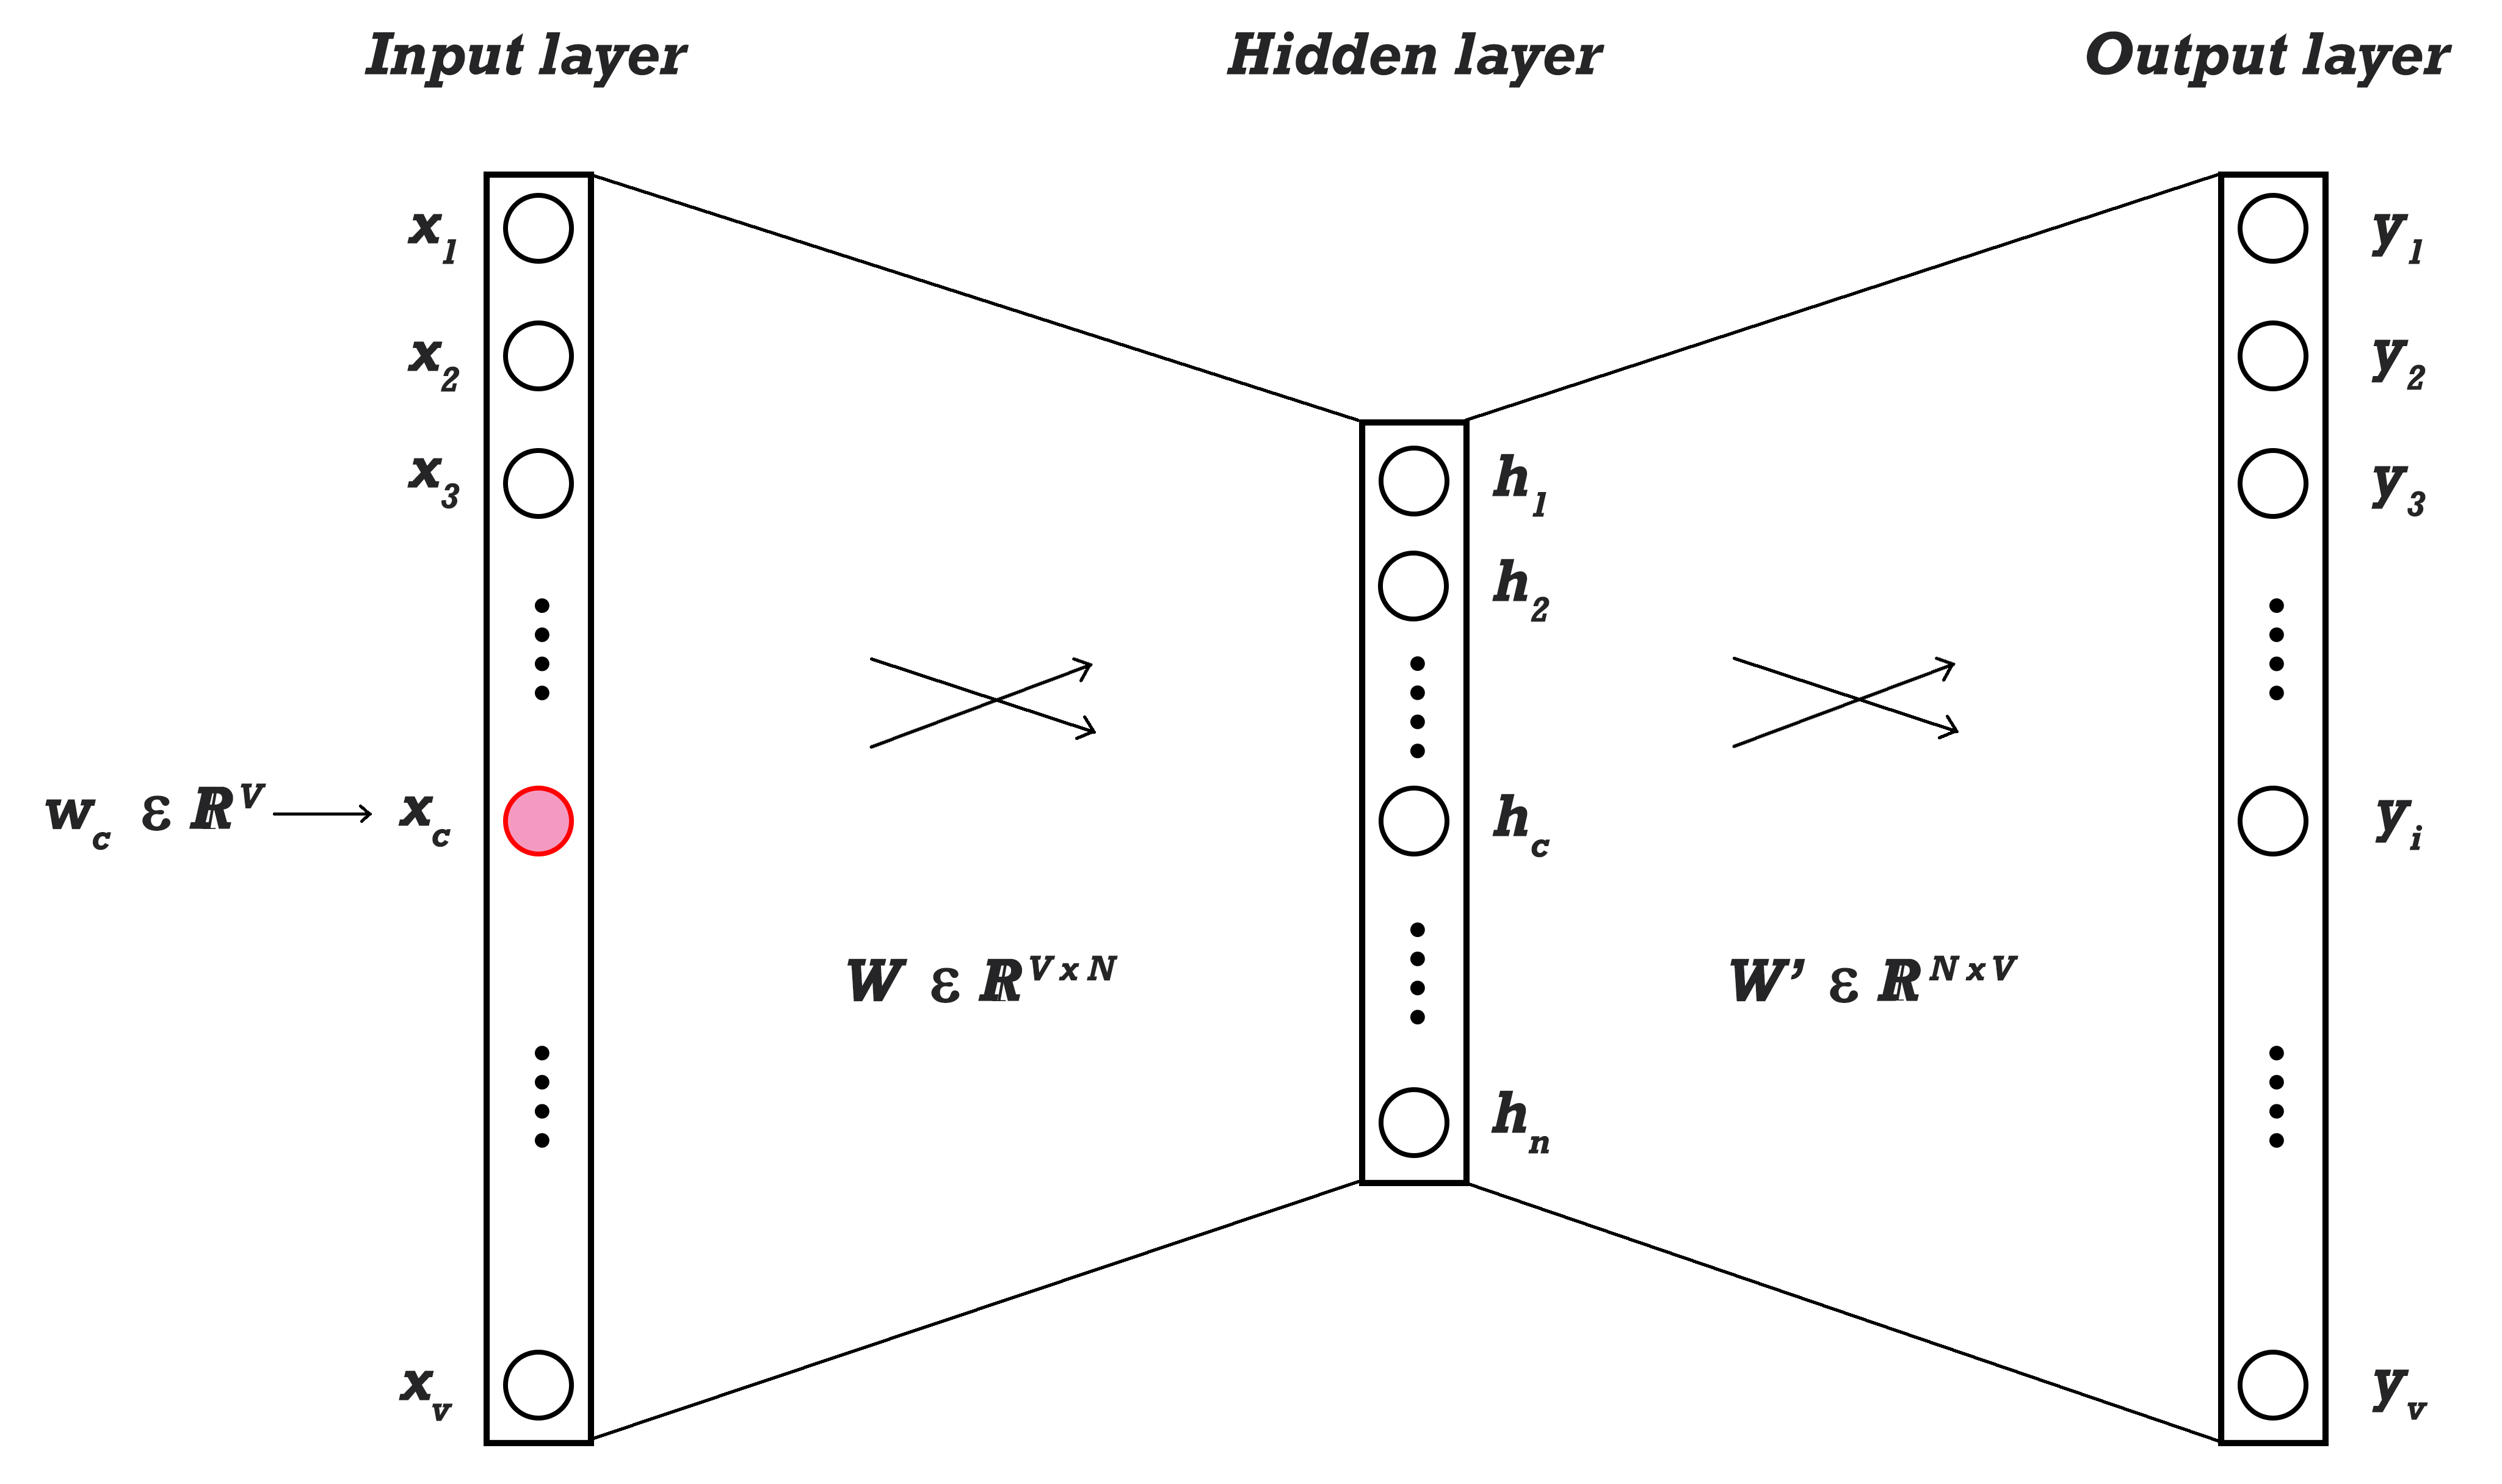
\includegraphics[width=0.8\linewidth,height=10cm,keepaspectratio]{cbow}
\caption[The CBOW model]{\textbf{The CBOW model: } In the CBOW model, the objective is to predict the target word from the words in the context (or neighbouring words). The context words are input to the model (in this case only one) using localist representation where only one vector element corresponding to input word is active ($x_{c}$, shown in red). The model outputs the probability for each word in vocabulary, which is maximized for actual target word during training. Adapted from [ref].}
\label{fig:cbow}
\end{figure}

\begin{figure}[hbtp]
\centering
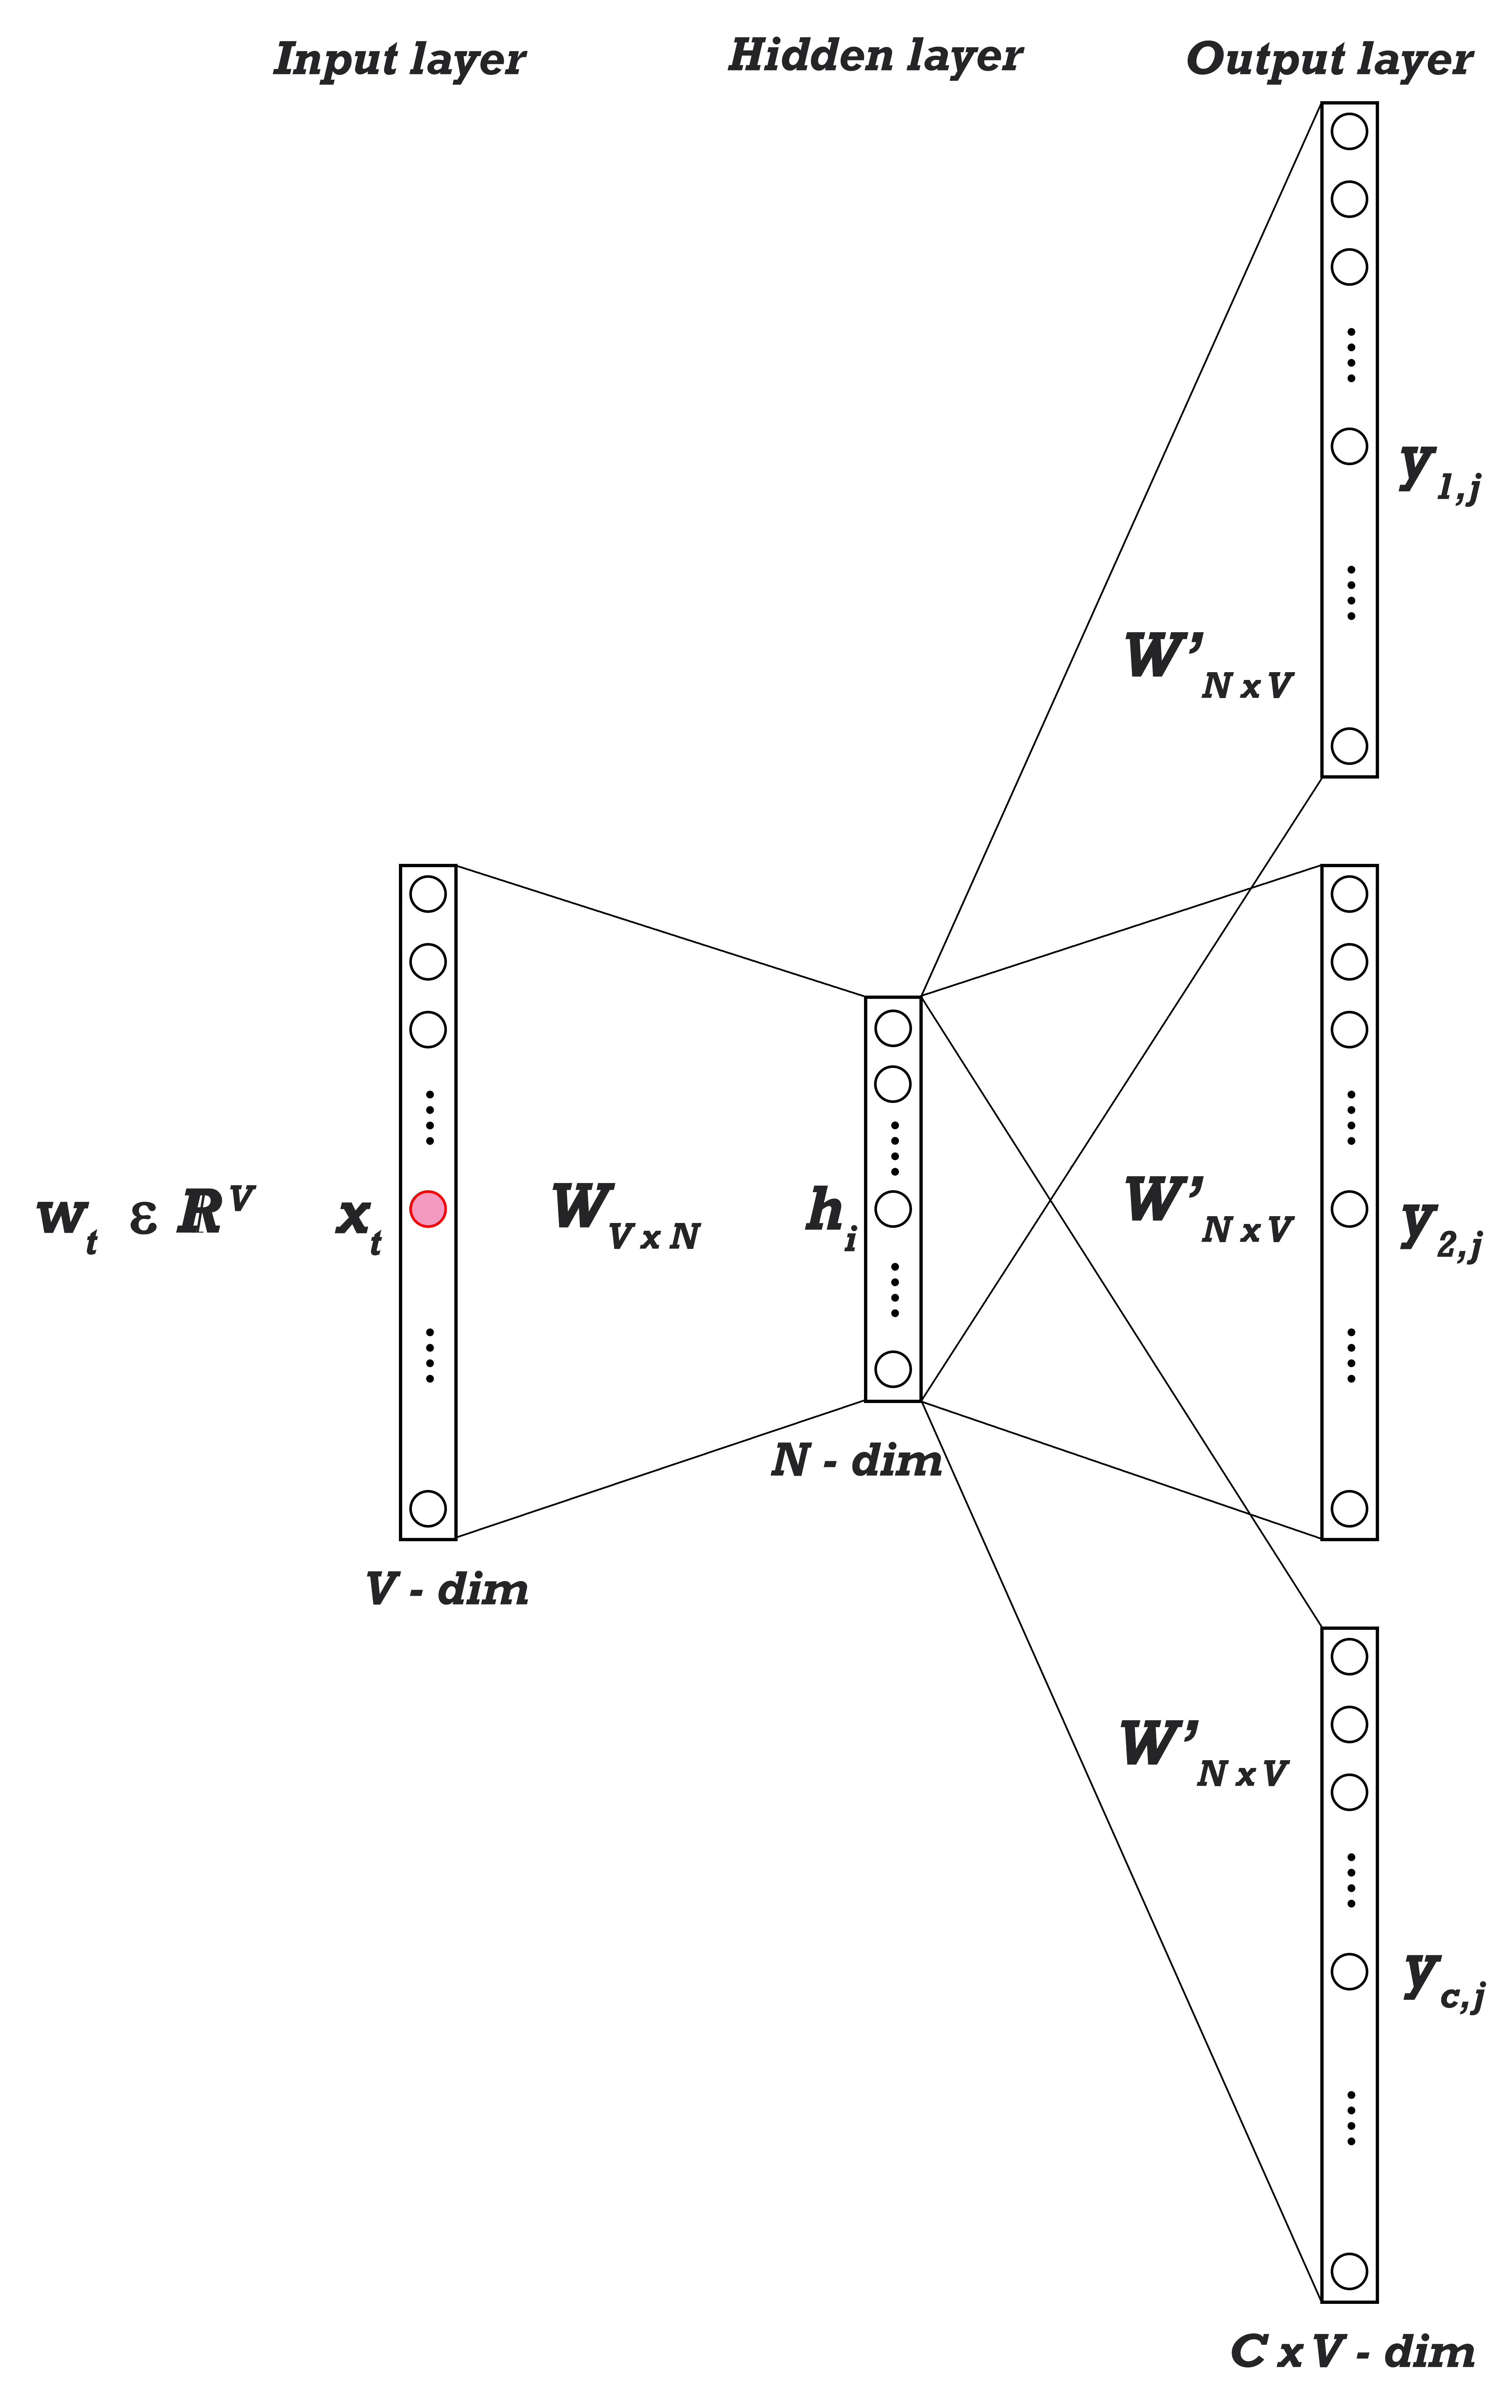
\includegraphics[width=1.8\linewidth,height=10cm,keepaspectratio]{sg}
\caption[The Skip-gram model]{\textbf{The skip-gram model: }In the skip model, the objective is reverse of CBOW. It predict the context words from the word. The target word is input to the model using localist representation where only one vector element corresponding to input word is active ($x_{t}$, shown in red). The model then maximizes the probaility of context words during training. Adapted from [ref].}
\label{fig:sg}
\end{figure}

\subsection{CBOW Model}

CBOW  model is a three layered neural model with the training objective to predict a target word (e.g. Peter) given some context words (John gave ball to …). Figure \ref{fig:cbow} shows the CBOW network architecture with a simplified case of one context word. The model is trained on the dataset having a vocabulary size $V$ in an unsupervised way to achieve the objective. The hidden layer is of size $N$, the dimensions of desired word embedding, and neurons in both the adjacent layer i.e. input and output layers,  are fully connected to hidden layer neurons. The input to the network is the context word $w_c {\in} \mathbb{R}^{V}$ and is represented using localist representation where only one unit $x_c$ at index c will be 1 out of V units $w_c=[{x_1,.....,x_V}]$ and all other units will be 0 \cite{w2v:parameter_learning}. The activation of hidden layer is then given by :

\begin{equation}\label{eqn:hidden_act}
	h = W^T . w_c= W_{(c,:)}=v_{c}
\end{equation}

where $W {\in} \mathbb{R}^{V{\times}N}$ is the weight matrix from input to hidden layer and $v_{c}$ is the vector embedding of the context word $w_c$. Eqn. \ref{eqn:hidden_act} basically copies the $c^{th}$ row of weight matrix $W$ on the hidden layer as hidden layer activation function is linear. 

A score $u {\in}\mathbb{R}^V$ is then calculated for all the target words in the vocabulary, which is essentially the compatibility of a word $w_i$ given the context word $w_c$.

\begin{equation}
\begin{split}
		 u &={W^{'}} ^ T . h \\
	   	   &= {W^{'}}^T. v_{c}	
\end{split}
\end{equation}

\begin{equation}
	u_i = {W^{'}_i}^T. v_{c}
\end{equation}

\noindent  where $u_i$ gives the score of $i^{th}$ word,$w_{i}$, for i = 1, 2...V. $W^{'}{\in} \mathbb{R}^{N{\times}V} $ is the weight matrix between hidden and output layer. ${W^{'}_i}$ is the $i^{th}$ column vector of matrix $W^{'}$.  
The computed scores are then converted to posterior probabilities by output neurons with softmax activation function. Thus aliasing ${W^{'}_i}$ as $v^{'}_{i}$ we get output probabilities as: 

\begin{equation}
\begin{split}	
y_i &= P(w_i | w_c) = \frac {\exp(u_i)} {\sum_{i' {\in} V} \exp (u_{i^{'}})}\\
	&= \frac {\exp({v^{'}_{i}}^T.v_{c})}{\sum_{i' {\in} V}\exp({v^{'}_{i^{'}}}^T.v_{c})}
\end{split}
\end{equation}
where $y_i$ is the probability of $i^{th}$ word given the context word.

The training objective is then achieved by maximizing the log likelihood of actual target word $(w_{t})$ given the context word ($w_{c}$). So the cost functions can be written as:

\begin{equation}
  \begin{split}
  	J_{ML} &= max \log P(w_t | w_c) \\
		   &= {v^{'}_{t}}^T.v_{c}- \text{ log} \sum_{i' {\in} V} {\exp({v^{'}_{i^{'}}}^T.v_{c})}
  \end{split}
\end{equation} 

In case of multiple context words is input to the network, the equation \ref{eqn:hidden_act} only change to:

\begin{equation}
h= \frac {1}{K} .(v_{c_1}+v_{c_2}+.......+v_{c_K}) 
\end{equation}	

where $k$ is the size of context window. This equation averages vector embeddings of all context words \cite{w2v:parameter_learning}.

\subsection{Skip-gram Model}

In the Skip-Gram model training objective is reversed from that of CBOW model. In other words, the objective is to learn the vector representation of the word that is good in predicting the context words \cite{w2v:mikolov_2013_distributed}. Thus for a given sequence of words $\{w_1,.....w_V\}$, the objective is to maximize the average log probability. 

\begin{equation}
\frac {1}{V}\sum_{t=1}^{V} \sum_{{-c \leq j \leq c},{j \neq 0}} {log\ P(w_{t+j}|w_t)}
\end{equation}

where c is the size of context window, $P(w_{t+c}|w_t)$ is the probability of context word $w_{t+j}$ for $-c \leq j \leq c$, given the target word $w_t$. This is measured using softmax function as:

\begin{equation} \label{eqn:sg_prob}
p(w_{t+j}|w_t)=\frac {\exp({{v^{'}_{t+j}}^{T}}.{v_t})}{\sum_{w {\in}V} \exp({{v^{'}_{w}}^{T}}.{v_t})}
\end{equation}

\noindent where ${v^{'}_{t+j}}$ and ${v_t}$ are the vector representation of word $w_{t+j}$ and $w_{t}$ respectively.

The objective function is thus optimized using stochastic gradient descent to learn the good word vectors. Calculating the full softmax is computationally expensive as it need to compute and normalize probability for every other word $w$ in the vocabulary V for a given input word ($w_{c}$ for CBOW or $w_{t}$ for skip-gram) at every training step. Thus negative sampling was proposed for learning the word embeddings\cite{w2v:mikolov_2013_distributed}.

\subsubsection{Skip-gram with negative sampling}

For learning word features full probabilistic models was not required. So in skip-gram negative sampling is used for approximation of word features. This technique treats feature learning as a binary classification (logistics regression) problems \cite{w2v:mikolov_2013_distributed, w2v:tensor_flow}. The model is thus trained to distinguish the target word from $k$ imaginary noise words $w_{noise}$, in the same context. Thus the log probability $p(w_{t+j}|w_t)$ in equation \ref{eqn:sg_prob} is now approximated by:

\begin{equation}
p(w_{t+j}|w_t)=log\ \sigma({{v^{'}_{t+j}}^{T}}.{v_t})\ +\  \sum_{w_{noise}{\in}N_{k}} \log\ \sigma({{v^{'}_{noise}}^T}.v_{t})
\end{equation}

\noindent where $\sigma(x)=1/(1+\exp(-x))$, and $N_k$ is the set of $k$ noise word compared to corresponding context word $w_{t+j}$ for $-c \leq j \leq c$. 

\subsection{Properties of Word2Vec embeddings}

Although the word2vec model is simple in architecture and easy to train, it produces word vector embedding which surprisingly encodes several linguistic regularities and patterns \cite{w2v:language_similarities, w2v:mikolov_2013_distributed}. More importantly it is astonishing because the network was not explicitly trained for these linguistic properties (see fig. \ref{fig:sem_rel} and \ref{fig:w2v_translation}). The distributed word embeddings encodes semantic and syntactic properties of the words as a constant vector offset between a pair of words sharing a specific relationship\cite{w2v:mikolov_2013_distributed}. For example, the word embeddings $"King - Queen \approx man - woman"$, $"apples - apple \approx cars - car"$, $"walking - walked \approx swimming - swam"$.

\begin{figure}[hbtp]
\centering
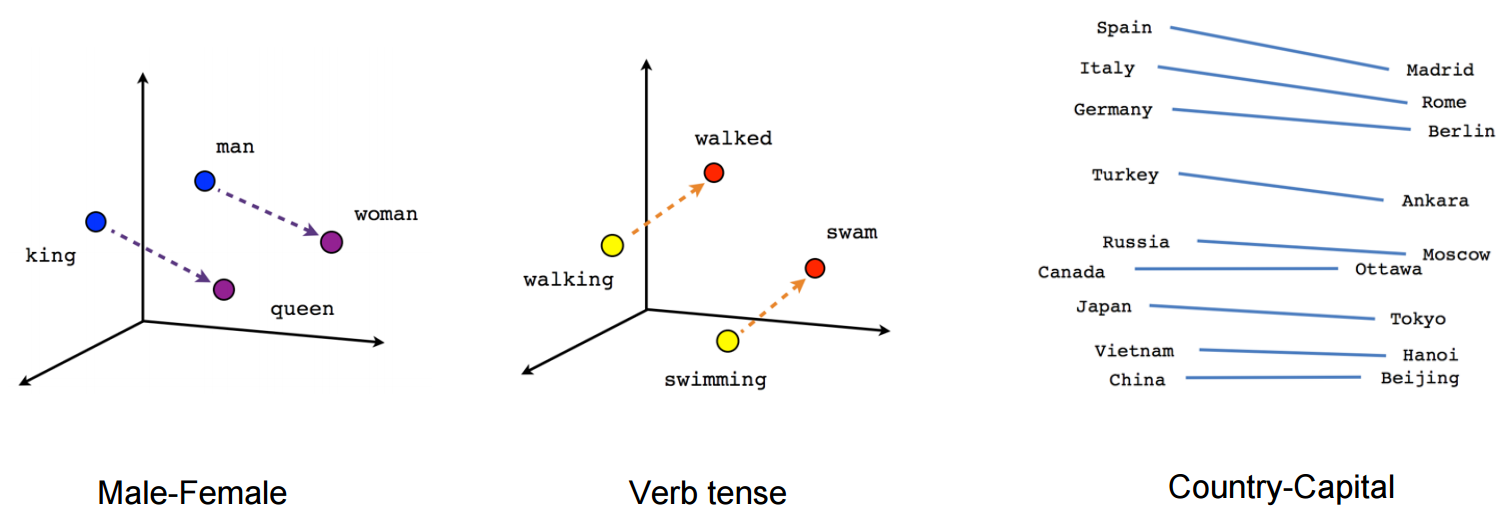
\includegraphics[width=0.8\linewidth]{linear-relationships}
\caption[Word2vec semantic regularities]{\textbf{Word2vec semantic regularities.}} 
\label{fig:sem_rel}
\end{figure}

\begin{figure}[hbtp]
\centering
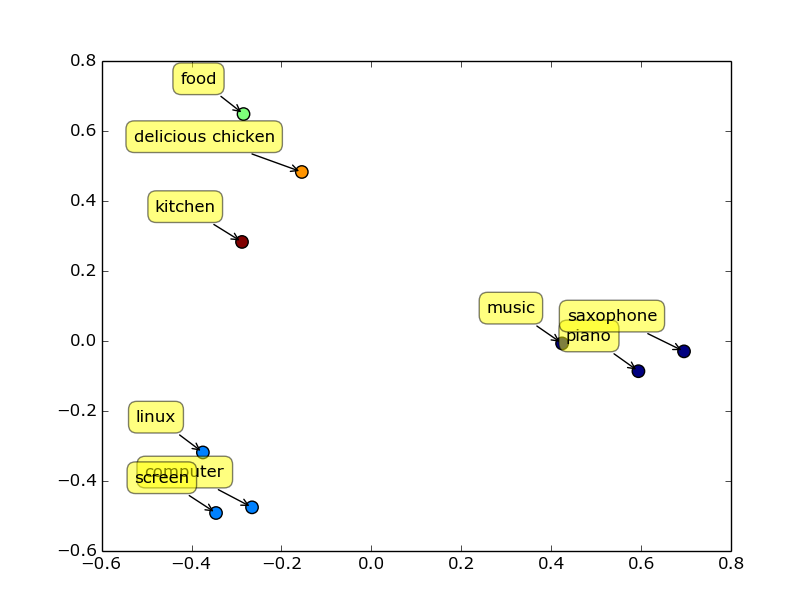
\includegraphics[width=0.8\linewidth]{word2vec_clustering}
\caption [Word2Vec word clustering]{\textbf{Word Clustering with word2vec word embedding:} The figure shows the word clustering property obtained by projecting the word vectors on two dimesional space using PCA. The words vector taken from pretrained word2vec Google News corpus\footnotemark }
\label{fig:w2v_clustering}
\end{figure}

\footnote{https://drive.google.com/file/d/0B7XkCwpI5KDYNlNUTTlSS21pQmM/edit}

\begin{figure}[hbtp]
\centering
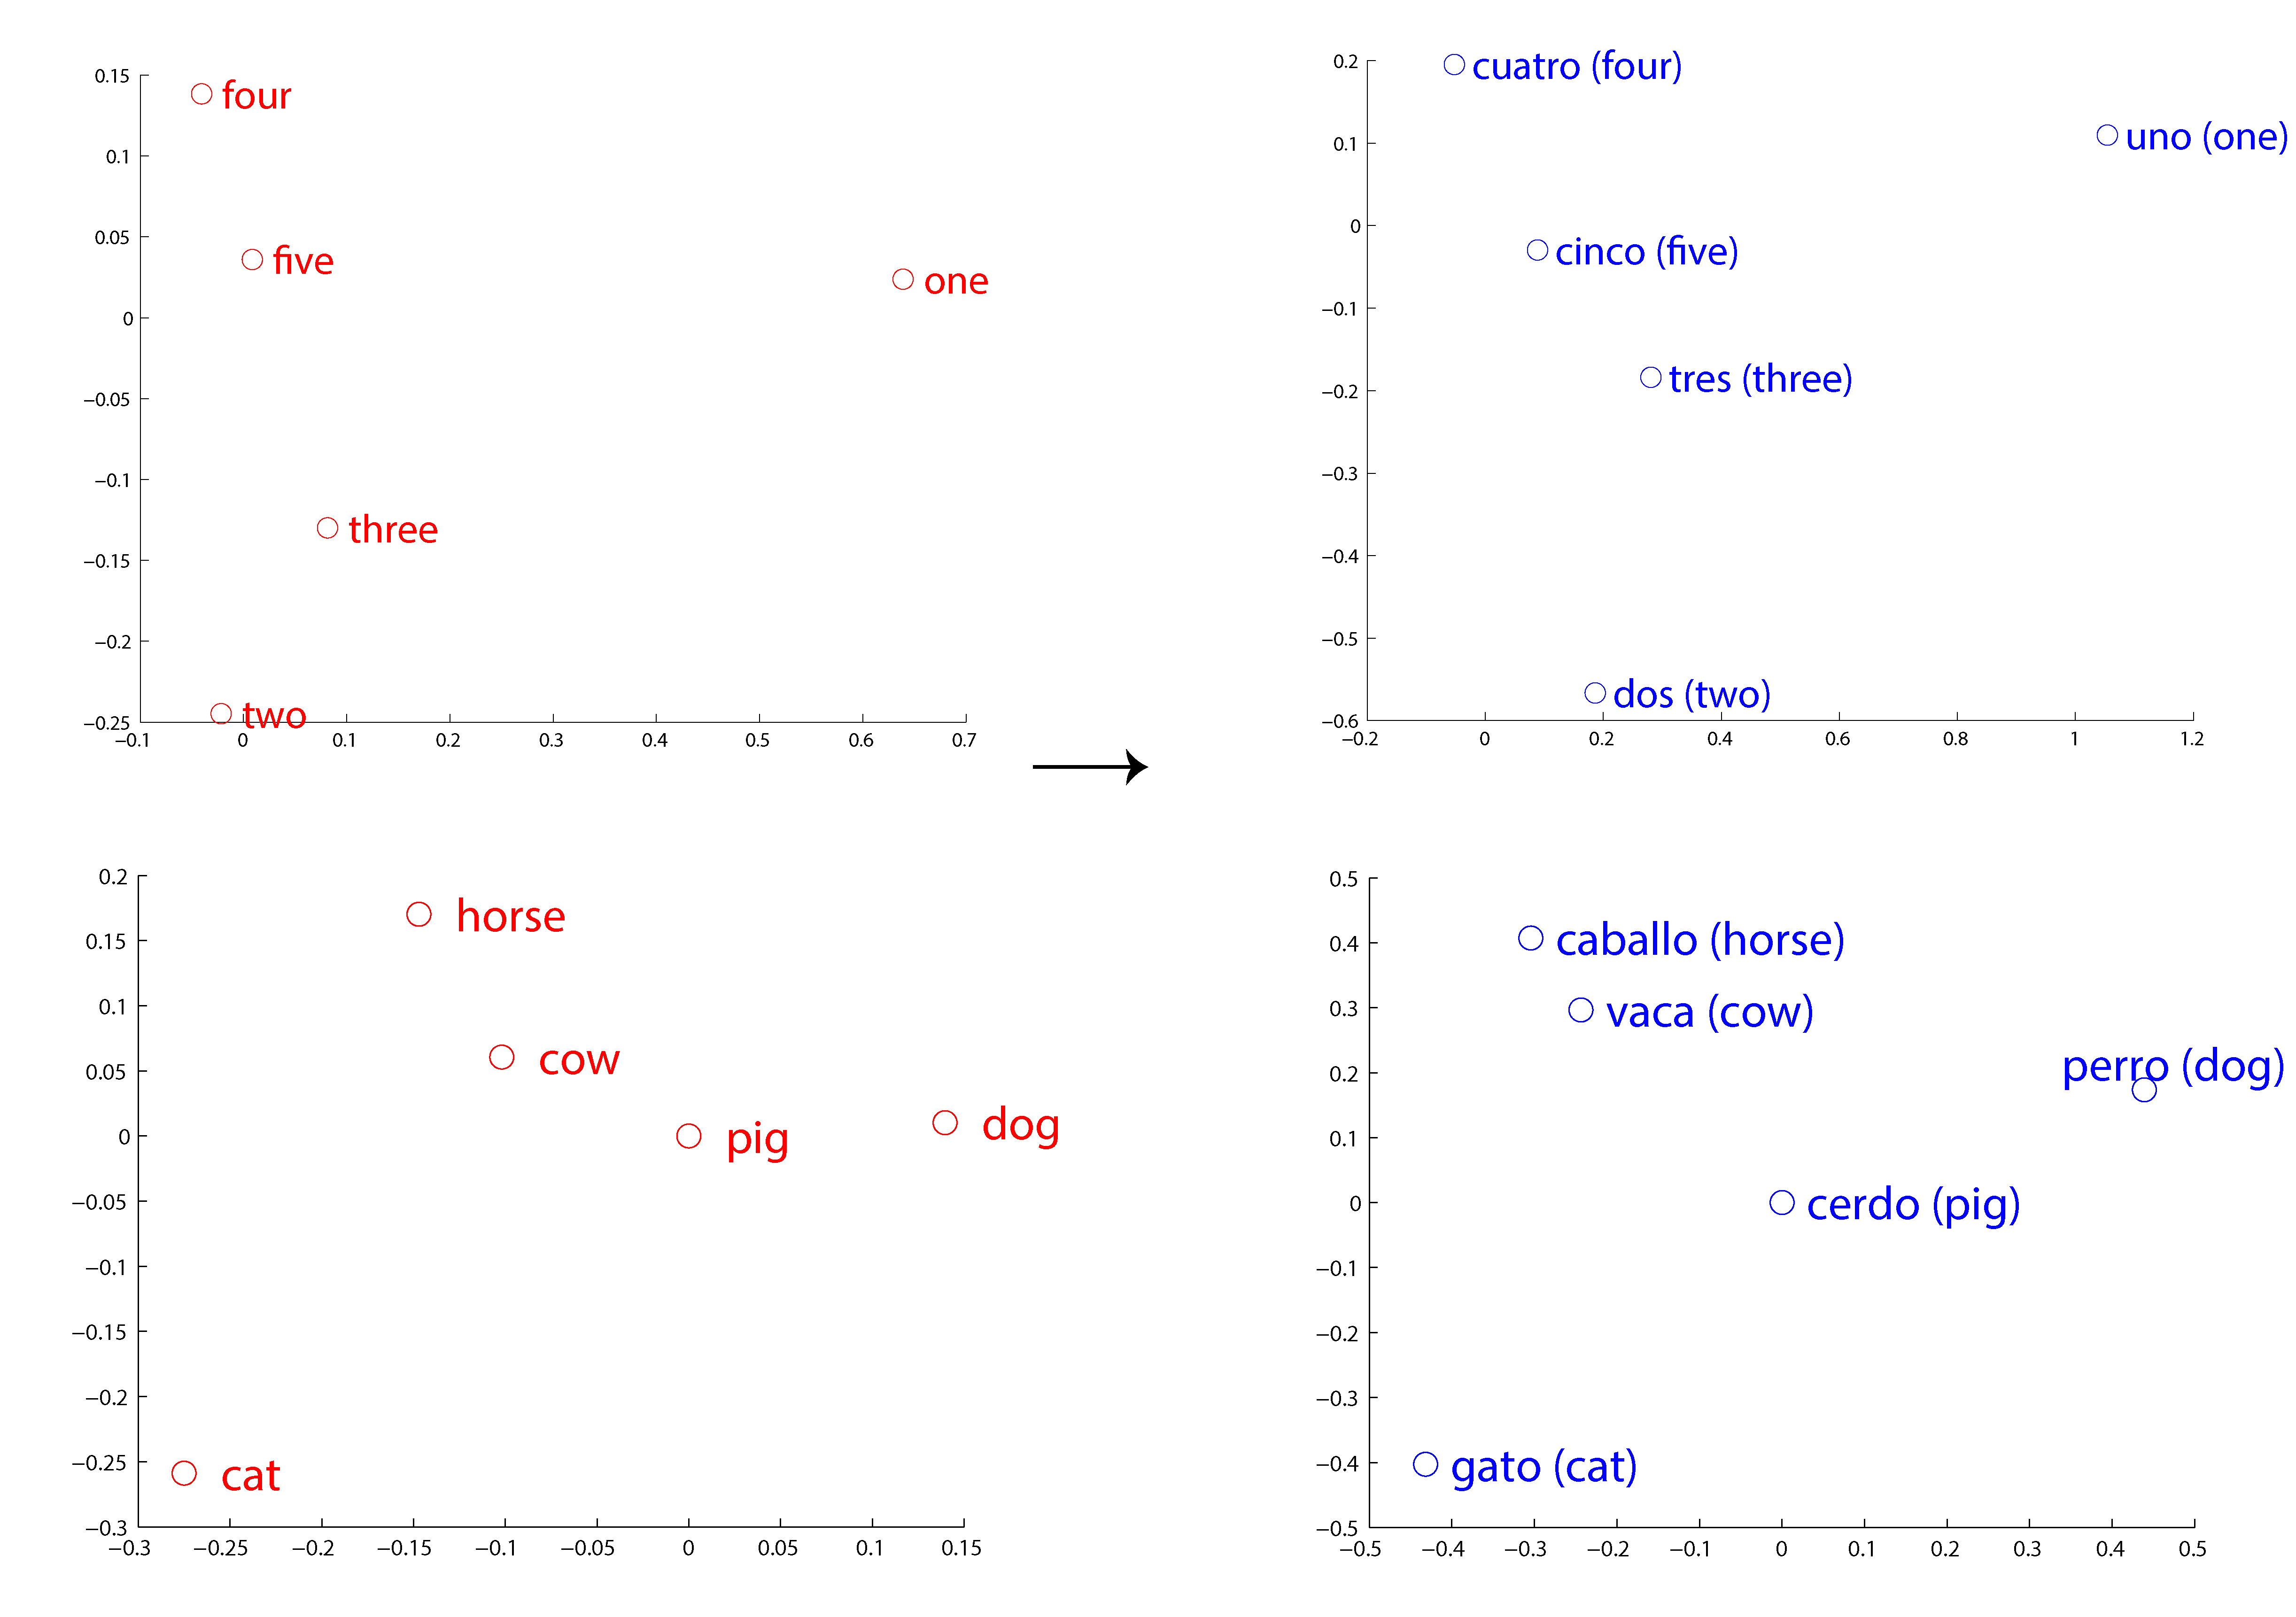
\includegraphics[width=0.8\linewidth,height=10cm,keepaspectratio]{word2vec_translation}
\caption[Word2Vec language translation property]{\textbf{Word2Vec language translation property.}}
\label{fig:w2v_translation}
\end{figure}

The another interesting property is that the the semantically related words are placed close to each other in word vector space, thus forming clusters of semantically related words. It was also observed the word embeddings of similar words in different languages have the same geometrical arrangement in embedding space of respective language. Thus it is also possible to learn linear mapping between different embedding space by vector rotation and scaling \cite{w2v:language_similarities}. Several other regularities can also be captured by performing basic linear operation on word-embeddings \cite{w2v:mikolov_2013_distributed}. 

\section{Echo State Network (ESN)}

Echo State Network (ESN) is a network with a new viewpoint on Recurrent Neural Network (RNN). It is a discrete time continuous state recurrent neural network introduced by Herbert Jaeger \cite{esn:jaeger:2001} and is believed to closely resemble the learning mechanism in biological brains. ESN is found to be computationally simple and inexpensive to process the temporal or sequential data. The main idea of ESN is to operate the random, large, fixed RNN with the input signal and the non-linear response generated by each neuron of the RNN is collectively combined with the desired output signal using regression to learn the output weights \cite{esn:jaeger_tutorial, esn:jaeger:2001,esn:scholarpedia:2007}.

\subsection{ESN Architecture}

ESN is surprisingly efficient variant for RNN training (see fig. \ref{fig:esn_arch}). In the standard RNN all the weights are required to be tuned even-though it was shown that RNN works well enough even without full adaptation of weights. The classical ESN mainly contains three layers, input layer, the hidden layer (also known as reservoir) and the readout layer. The input layer is fully connected to the hidden layer and both the hidden layer and the input layer is connected to the output layer. The output layer is fully connected back to the hidden layer. However the connection from input to output layer and output layer to hidden layer is optional and depends on the task.

The weights from input to reservoir (i.e. $W^{in}$) and from reservoir to reservoir (i.e. $W^{res}$), are sparsely and randomly initialized and more crucially remains untrained during training. The non-zero element in sparse input weight matrix $W^{in}$ and reservoir weight matrix $W^{res}$ are generated from uniform or normal distribution. The weights from the reservoir to output layer (i.e. $W^{out}$) are the only weights learned during supervised training \cite{esn:jaeger:2001, esn:practical_guide}. For ESN approach to work the reservoir should possess the Echo State Property: if a long input sequence is given to the reservoir the reservoir will end up in the same state irrespective of the initial reservoir state. In other word the reservoir states 'echoes' the input sequence and the effect of previous reservoir state and the previous input on the future reservoir states should vanish gradually \cite{esn:practical_guide, esn:jaeger_tutorial}. 

\begin{figure}[hbtp]
\centering
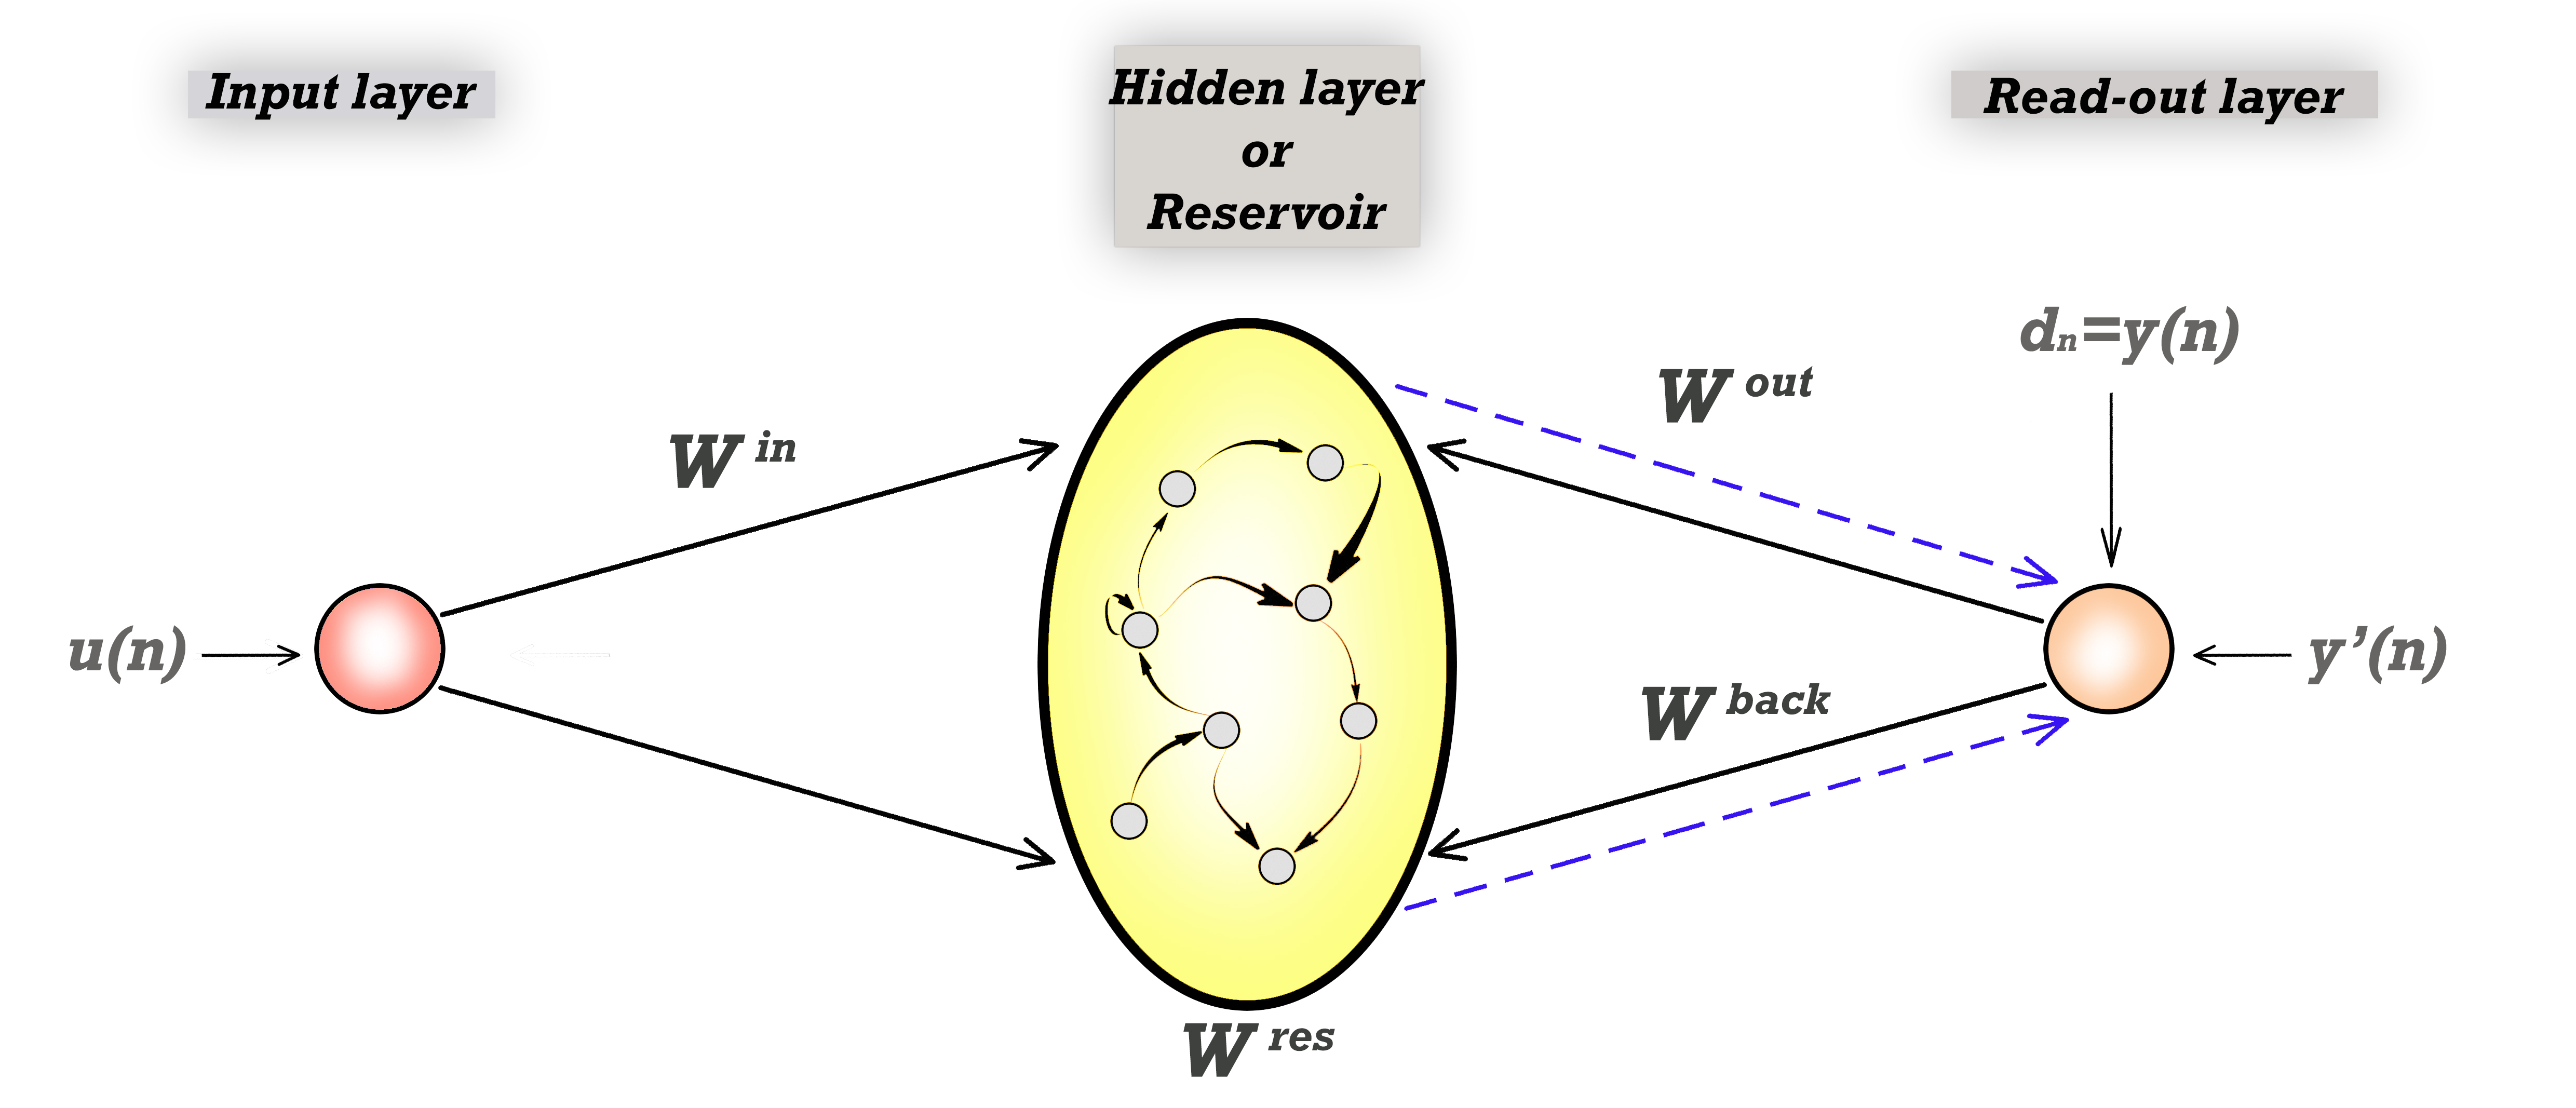
\includegraphics[width=0.8\linewidth]{esn_architecture}
\caption[Architecture of classical ESN]{\textbf{Architecture of classical ESN:} The reservoir is the recurrent neural network with $N_{x}$ units and initialized with random connection. The reservoir is provided input $u(n)$ to the input layer and teacher layer $y(n)$ are pushed output neurons  respectively during training. The input to reservoir weights ($W^{in}$), output neurons to reservoir ($W^{back}$, optional and depends on task) and reservoir to reservoir weight ($W^{res}$) from are also randomly initialized and stays static during learning. The output weight from reservoir to output unit are the only weights learned by the network during training. Adapted from \cite{esn:practical_guide}}
\label{fig:esn_arch}
\end{figure}

To ensure the echo state property in ESN, firstly, the reservoir weights matrix $W^{res}$ and the input weights matrix $W^{in}$ are often generated sparsely (i.e. most of the elements in these matrices will be zero) and randomly from a normal or uniform distribution \cite{esn:practical_guide}. The input weight matrix is however a bit more denser than the reservoir weight matrix. The sparsely generated random reservoir weights matrix $W^{res}$ is often scaled such that its spectral radius $\rho(W^{res})$ i.e. largest absolute eigenvalue, is less than one. To scale the randomly generated $W^{res}$ matrix, it is first divided by its spectral radius and then multiplied with desired spectral radius \cite{esn:jaeger_tutorial}.

\begin{equation}\label{eqn:res_scaling}
W_{new}^{{res}}=\gamma \frac{W^{res}}{\rho(W^{res})}
\end{equation}

where $W_{_{new}}^{{res}}$ is the scaled reservoir weight matrix, $0 < \gamma < 1$ is the desired spectral radius and $\rho(W^{res})$ is the spectral radius of randomly generated reservoir Matrix $W^{res}$.

It is also argued that the $\rho(W^{res}) < 1 $ is not a necessary condition for ESN to have the echo state property and can be achieved even when $\rho(W^{res}) > 1$ \cite{esn:jaeger:2001, esn:practical_guide, esn:jaeger_tutorial}. Intuitively, the spectral radius is a crude measure of the amount of memory the reservoir can hold, the small values meaning a short memory, and the large values a longer memory, up to the point of over-amplification when the echo state property no longer holds. The input weights are also scaled to regulate the non-linearity in reservoir activations. A very high input scaling let the reservoir to behave in highly non-linear manner (because of tanh activation function) whereas a very small input scaling is used wherever linearity is required in a task \cite{esn:practical_guide}.

\subsection{Training ESN}\label{ssec:esn_training}

ESNs are mostly applied supervised machine-learning tasks where temporal or sequentail aspect of the data is to be modeled. Before training, the reservoir of size $N_{x}$, generally containing leaky-integrated discrete-time continuous-value neurons with \textit{tanh} activation function is generated. The reservoir of any computationally affordable size can be used. The bigger the reservoir size, the more the input signal gets non-linearly expanded and easier it will be to find linear combination with the desired output signal \cite{esn:practical_guide, esn:jaeger_tutorial}. With the big reservoir size comes the risk of over-fitting. Thus, It is also important to use proper regularization methods to avoid over-fitting. The reservoir weight $W^{res}$, input weights $W^{in}$ and $W^{back}$ are then randomly initialized.

The training objective of ESN approach is to learn a model which outputs $\textit{y'}$, such that it is as close as possible to the target output \textit{y} by mining the error measure $E(y',y)$ and also generalize well on the data not used for training. Root Mean Square Error is typically chosed as erorr measure E. Thus during training, the given training input signal $\textit{u(n)} \in \mathbb{R}^{N_u}$ and the corresponding teacher signal $\textit{y(n)} \in \mathbb{R}^{N_y}$  is input to the reservoir at every time-step 'n'. Here n = 1,2...,T is the discrete time step for sequence of length T. The reservoir then generate a sequence $\textit{x(n)}$ of $N_{x}$-dimensional reservoir states which is non-linear high dimensional expansion of the input signal $\textit{u(n)}$ \cite{esn:jaeger_tutorial}. The reservoir activation and reservoir state update is computed using following recursive equations:

\begin{equation} \label{eqn:res_update}
x'(n) =\textit {tanh } ( W^{res}x(n-1) + W^{in}.u(n) + W^{back}.y(n-1))
\end{equation}
\begin{equation} \label{eqn:res_state}
x(n) =\textit (1-\alpha) x(n-1) + \alpha x'(n)
\end{equation}

where $\textit{ x(n)}$ is the vector of reservoir neuron's activations and $\textit{ x'(n)}$ is its update at time step $\textit{n}$. \textit{tanh} is reservoir neuron activation function. $ W^{in} \in \mathbb{R}^{{N_x} \times{N_u}}$ and $ W^{res} \in \mathbb{R}^{{N_x} \times{N_x}} $ are input weights and reservoir weights matrices respectively. $ W^{back} \in \mathbb{R}^{{N_x} \times{N_y}} $ is the optional output to reservoir matrix \footnote{this weight matrix is not used in our model implementation}. $\alpha \in (0,1]$ is leaking rate of neurons.  

The leaking rate, $\alpha$, regulates the speed of reservoir update dynamics in discrete time. Smaller value of also induces slow reservoir dynamics thus ensuring the long short-term memory in ESN \cite{esn:practical_guide, esn:optimization_leaky_neurons}. The reservoir activation states are accumulated at every time step for regression with the teacher output. The linear readout weights are then learned using equations:

\begin{equation}\label{eqn:esn_output}
y'(n) = \textit W^{out}x(n)
\end{equation}

where $y'(n) \in \mathbb{R}^{N_y}$ is output of the network and $W^{out} \in \mathbb{R}^{{N_y} \times {N_x}}$ is the output weight matrix.

Writing the equation \ref{eqn:esn_output} in matrix form, the output weights $W^{out}$ are then learned using the following equation:
 
\begin{equation}
Y=W^{out}X
\end{equation}
\begin{equation}
W^{out}=YX^{T}(XX^{T}+{\beta}I)^{-1}
\end{equation}

where $\beta$ is the regularization coefficient parameter of ridge regression and \textit{I} is the Identity matrix. 

Training procedure of ESN, have only few global parameters which are to be optimized: reservoir size $ N_{x} $, spectral radius of $W^{res}$, input scaling of $W^{in}$, leak rate $\alpha$ and the ridge parameter $\beta$. All these parameters can only be optimized by trial and error method and depends heavily on the task under consideration. Usually a grid search is applied to explore the best parameter combination.   

\cleardoublepage

\chapter{Related Work and Open Issues}\label{issues}

Humans have a remarkable ability of perceiving and comprehending one or more languages. But how do they know what does a sequence of symbols means? In other words how do they link a sequence of words to its meaning? With this research question, Hinaut et al. \cite{xavier:2013:RT} proposed a neuro-inspired model, $\theta RARes$, to process the sentence across time without having to know the sematics of the words. The model used reservoir computing approach namely echo state network and implemented on robotics architecture \cite{tra:xavier_hri} for the thematic role assingment task. This was the first time when echo state network was used for thematic role assingment task. The experiments done for TRA showed the results toward modelling of language acquisition in brain \cite{tra:xavier_wermter:2014,xavier:2013:RT}. The model was based on the cue competition hypothesis of Bates et al. \cite{tra:bates:1982} which states that closed class words (e.g. prepositions, articles, determiners, pronouns etc.), the order of words and prosody in a sentence encodes the grammatical structure. This principle was then utilized for thematic role assingment task.

\section{Overview of $\theta RARes$ Model}

$\theta RARes$ Model is basically an echo state network, used to learn and predict thematic roles of the input sentences. The model is based on the notion of grammatical construction. The grammatical construction of a sentence is defined as the the mapping of surface form (word order) of sentence to its meaning \cite{gc:goldberg:1995}.Figure \ref{fig:tra_gc} represents the characterization of thematic role assignment in grammatical construction form. The model does not takes in input the raw sentences but instead use the abstract form of the sentences. The abstraction marks each word of a sentence into two kind of symbols: Function Words and Semantic Words. Semantic words are the open class words like nouns, verbs, adjectives, adverbs etc. whereas function words are closed class words like determiners, prepositions, articles, pronouns, verb inflexions like -ed,-ing or -s etc.. Thus before giving a sentence as an input to ESN, all the semantic words are replaced with a unique token 'SW' and pushed to FIFO memory stack(see fig. \ref{fig:xavier_model}). The functional words were left unchanged unchanged (see table \ref{tab:localist_representation}).

\begin{figure}[hbtp]
\centering
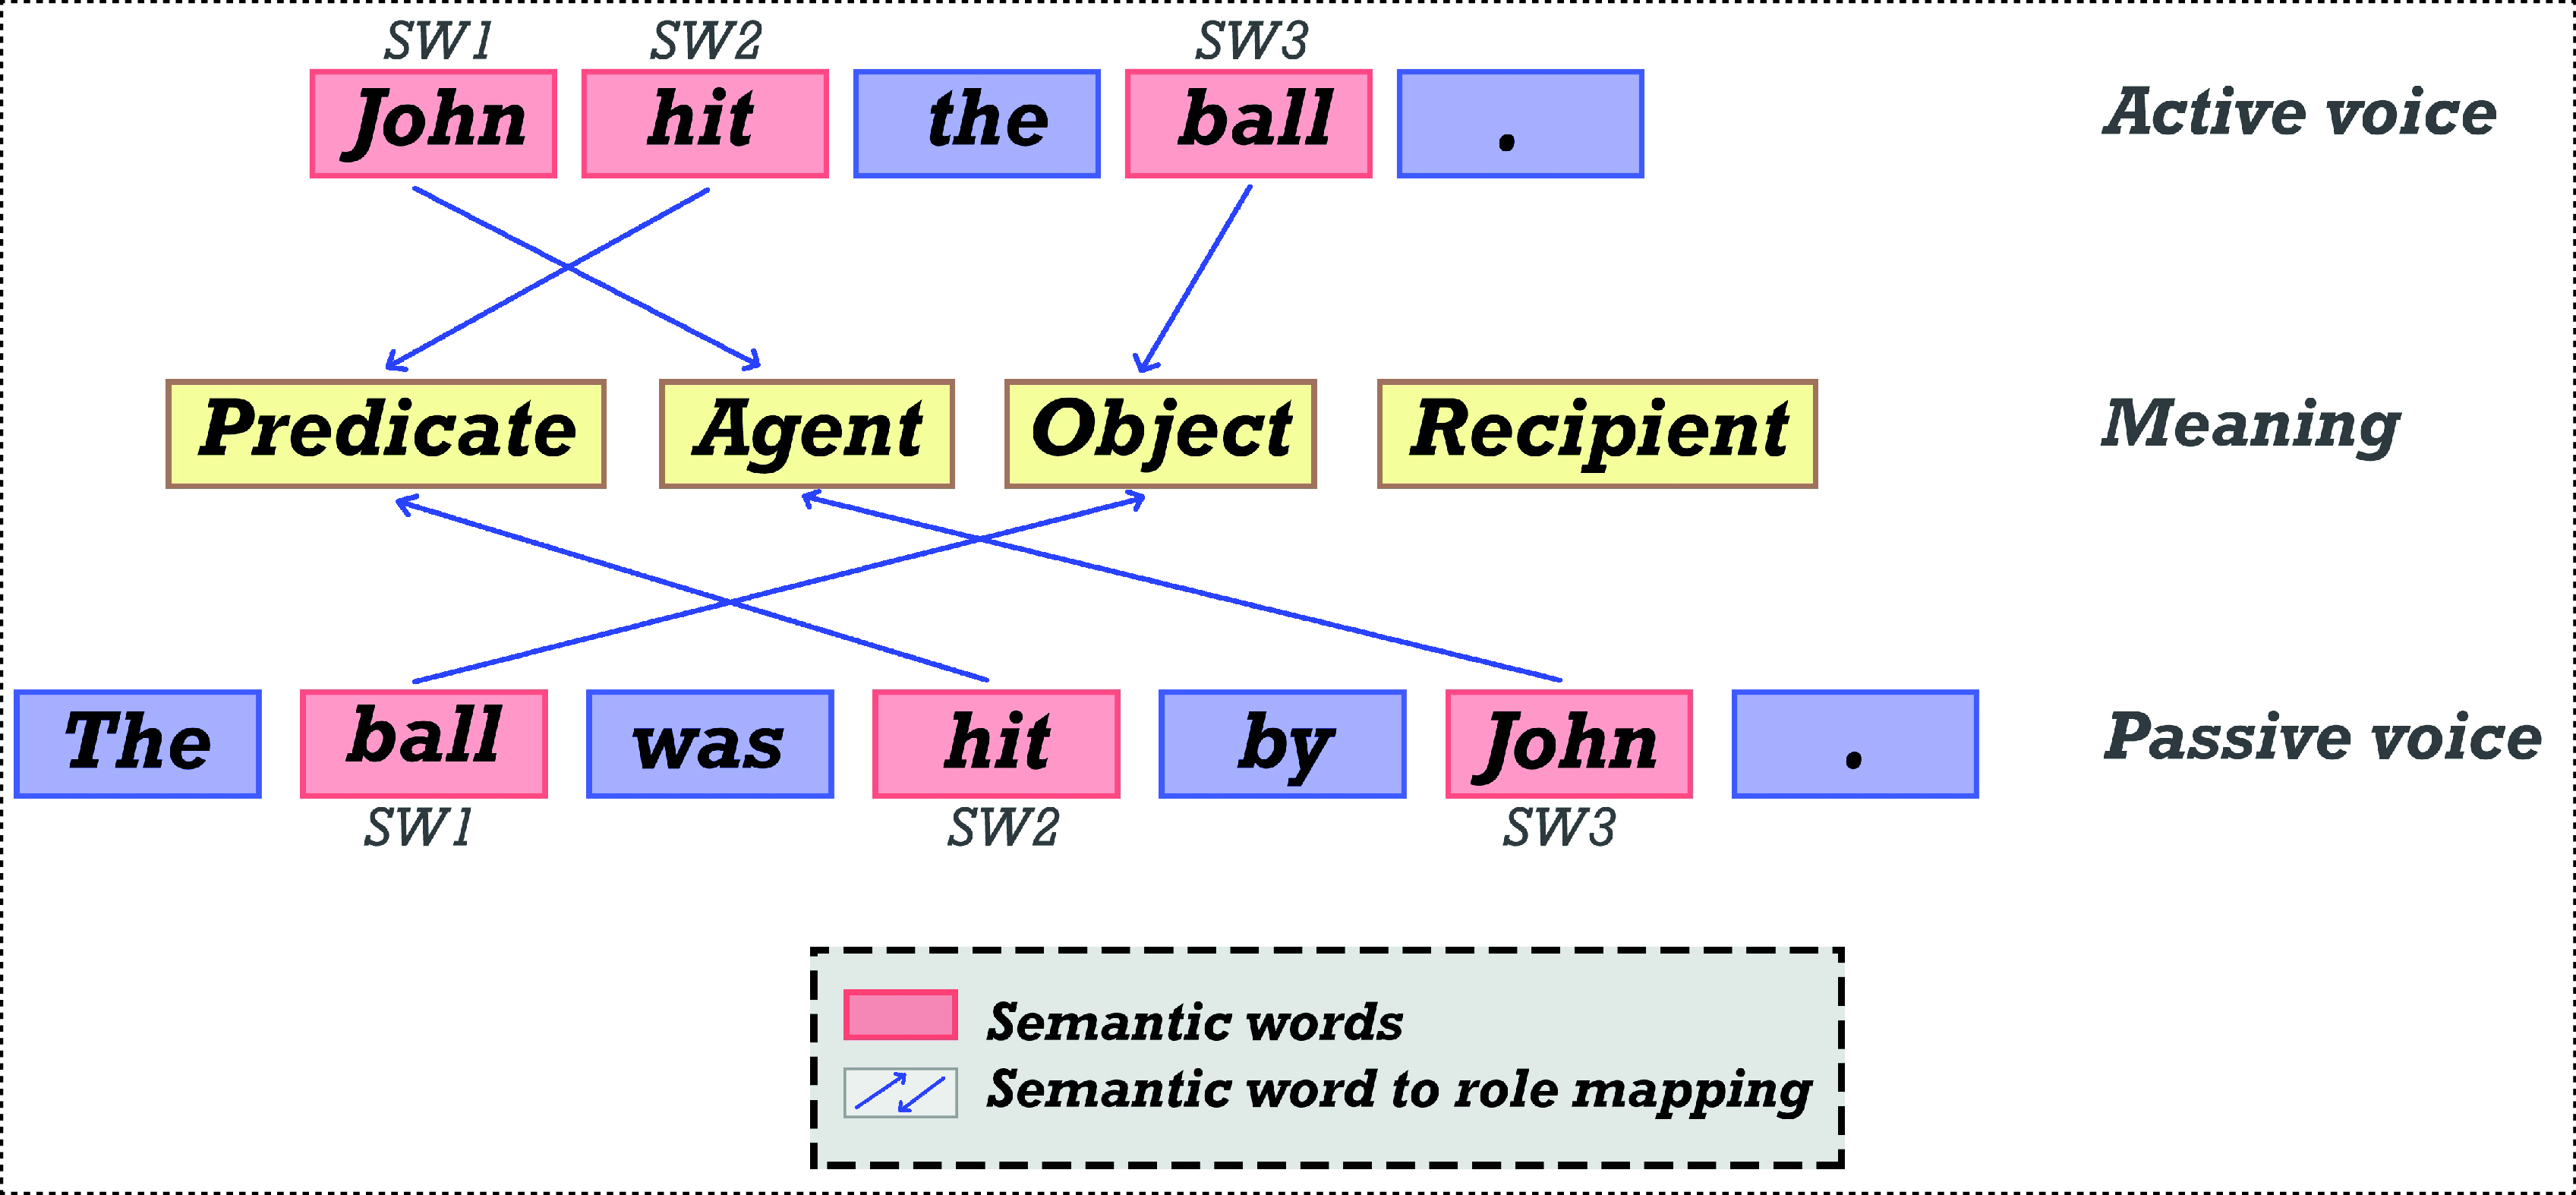
\includegraphics[width=0.8\linewidth,height=3.5cm, keepaspectratio]{grammatical_construction}
\caption[Word2vec semantic regularities]{\textbf{Word2vec semantic regularities.}} 
\label{fig:tra_gc}
\end{figure}

\begin{table}[hbtp]
\centering
\caption[Localist vector representation of sentence]{Transformation of a sentence by replacing semantic words with 'SW' token and localist vector representation of words used as an input for a sentence.}
\begin{tabular}{|c|c|c|c|c|c|c|c|}
\hline
\textbf{Original words} & \textbf{Transformed words}  & \multicolumn{6}{c|}{\textbf{Localist vectors}} \\ \hline
put		&	SW     & 0   & 1  & 0  & 1  & 0  & 1  \\ \hline
the		&	the    & 0   & 0  & 1  & 0  & 0  & 0  \\ \hline
ball	&	SW     & 0   & 1  & 0  & 1  & 0  & 1  \\ \hline
on		&	on     & 0   & 0  & 0  & 0  & 1  & 0  \\ \hline
the		&	the    & 0   & 0  & 1  & 0  & 0  & 0  \\ \hline
box		&	SW     & 0   & 1  & 0  & 1  & 0  & 1  \\ \hline
\end{tabular}
\label{tab:localist_representation}
\end{table}

\begin{figure}[hbtp]
\centering
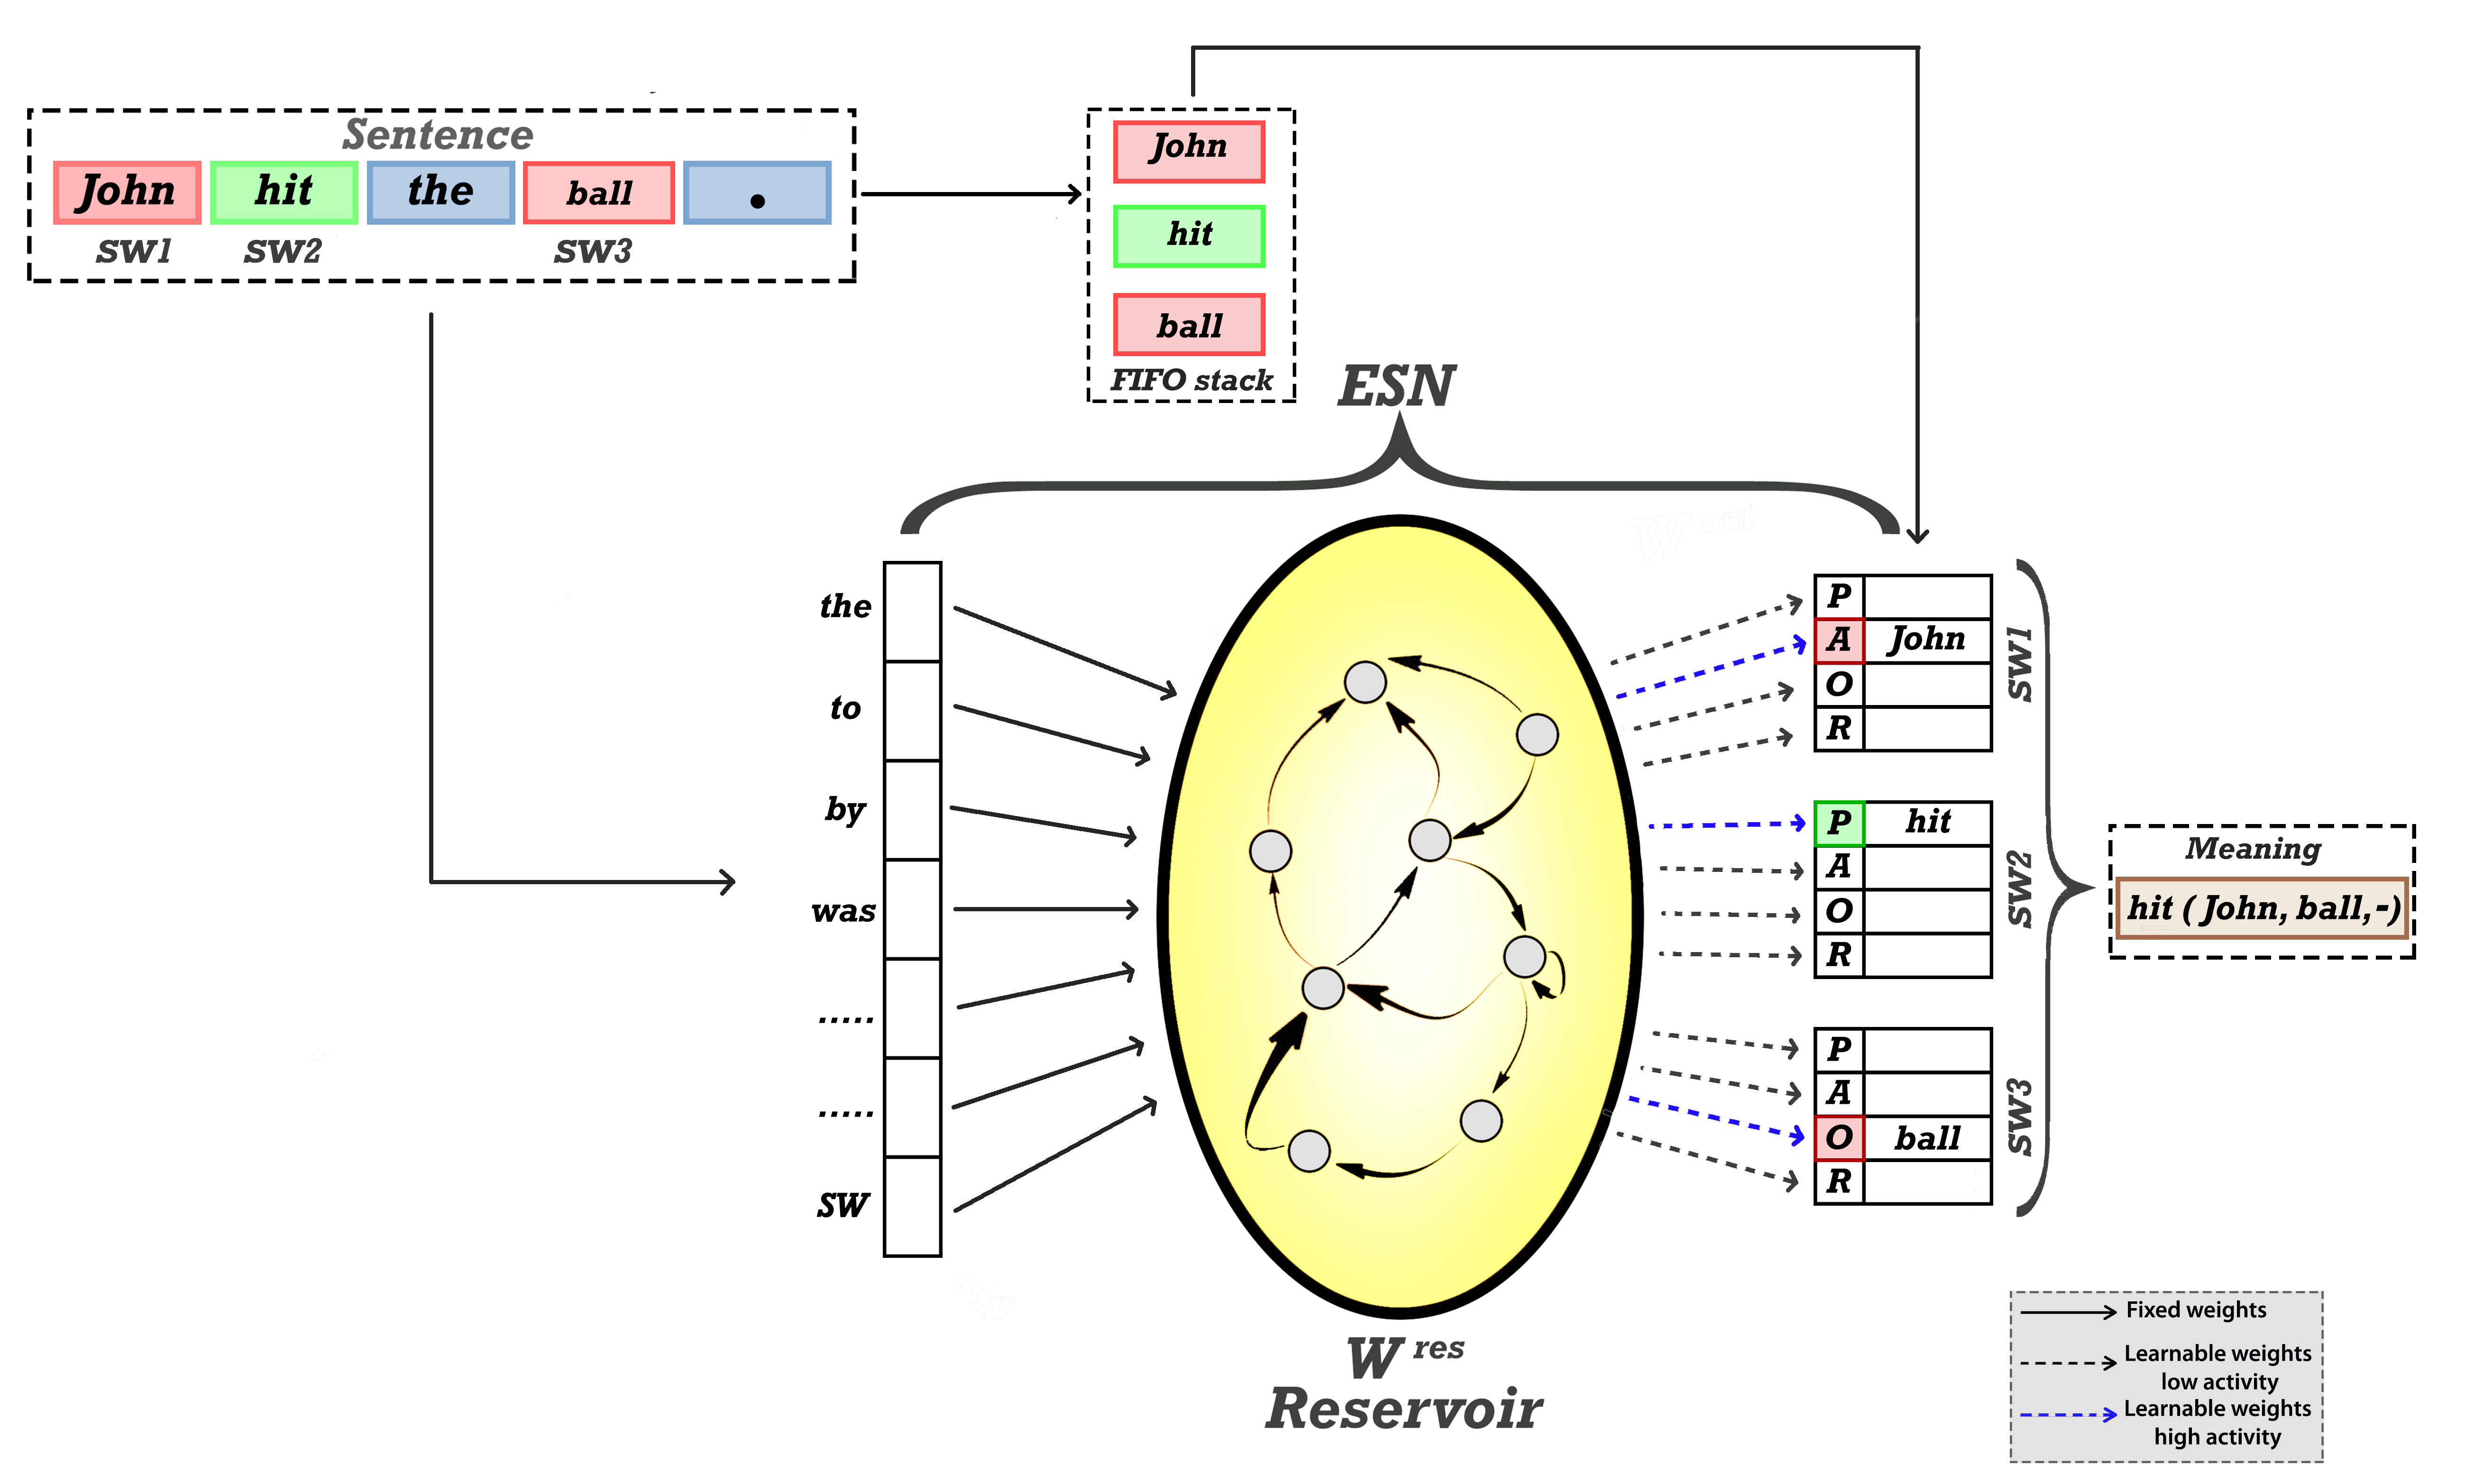
\includegraphics[width=0.8\linewidth]{xavier_model}
\caption[Word2vec semantic regularities]{\textbf{Word2vec semantic regularities.}} 
\label{fig:xavier_model}
\end{figure}

Thus for training the transformed sentences were presented to the model sequentially, word-by-word. Considering each word as a discrete atomic symbol, the words were encoded using localist vector representation, where all elements except the current input are zeros (see table \ref{tab:localist_representation}). Figure \ref{fig:xavier_model} shows the functional organization of the model. The localist word vectors are projected on the input layer of ESN and coded meaning of the input sentence is teacher-forced on the output layer of ESN. The model learns the thematic roles of all semantic words by learning reservoir to readout weights of ESN. During the testing the model predicts the coded meaning of the test sentence. The output activation is decoded to its meaning by thresholding the activation at last time step. For each SW word the that has highest activation is considered as the role of SW. Each semantic word in the memory stack is then mapped to the corresponding role (see fig. \ref{fig:xavier_model}). 

\subsection{Limitation of $\theta RARes$ model }

Transforming a sentence into its abstract representation (explained above) and using localist representation of each word in a sentence as an input to an ESN does not allow the network to leverage the information retrieved from semantically related words. The limitations for such an input representation mainly occurs with the ambiguous sentences. A sentence is said to be ambiguous if it has the same grammatical construction but different coded meaning and actual meaning. The limitation can be described below in the two ambiguous examples.

\paragraph{Example 1: Ambiguous Sentences}

\begin{enumerate}[noitemsep]
\item take (SW-1) the blue (SW-2) box (SW-3) \label{eg-1:sent-1}
\item take (SW-1) the left (SW-2) box (SW-3) \label{eg-1:sent-2}
\item throw(SW-1) the green(SW-2) box(SW-3)  \label{eg-1:sent-3} 
\end{enumerate}

All the three sentences having the same surface form after transforming the sentence by replacing the semantic words with 'SW' token i.e. SW the SW the SW SW.

\paragraph{Training with Sentence \ref{eg-1:sent-1}:} In the Sentence \ref{eg-1:sent-1} there are three semantic words namely SW-1: take, SW-2: blue, SW-3: box. During the training the sentence is input to the model from left to right word by word at each time step. The teacher output (thematic roles) of each semantic word is also teacher-forced as described below where, A: Action, O: Object, C: Color, I: Indicator. During the training ESN learns that second semantic word represents a \textit{'Color'}.

\begin{table}[hbtp]
\centering
\begin{minipage}{1.5in}
\begin{tabular}{|c|c|c|c|}
\hline
\multicolumn{4}{|c|}{\textbf{SW-1}}   \\ \hline
\textit{\textbf{A}}    & O & C & I 	\\ \hline
\textit{\textbf{take}} &   &   &  		\\  \hline
\end{tabular}
\end{minipage}
\begin{minipage}{1.5in}
\begin{tabular}{|c|c|c|c|}
\hline
\multicolumn{4}{|c|}{\textbf{SW-2}}                    \\ \hline
A	& O & \textit{\textbf{C}}    & I  \\ \hline
	&   & \textit{\textbf{blue}} & 	\\ \hline
\end{tabular}
\end{minipage}
\begin{minipage}{1.5in}
\begin{tabular}{|c|c|c|c|}
\hline
\multicolumn{4}{|c|}{\textbf{SW-3}}                                  \\ \hline
A	& \textit{\textbf{O}}   & C	& I \\ \hline
 	& \textit{\textbf{box}} &  	&   \\ \hline
\end{tabular}
\end{minipage}
\end{table}

\paragraph{Training with Sentence \ref{eg-1:sent-2}:} In the Sentence \ref{eg-1:sent-2} we have three semantic words; SW-1: take, SW-2: left, SW-3: ball. Both the sentences (\ref{eg-1:sent-1} and \ref{eg-1:sent-2}) differs only in the second semantic word. Now suppose we train this sentence with a teacher output as follows where symbols A, O, C and I have the same meaning as described above.

\begin{table}[hbtp]
\centering
\begin{minipage}{1.5in}
\begin{tabular}{|c|c|c|c|}
\hline
\multicolumn{4}{|c|}{\textbf{SW-1}}   \\ \hline
\textit{\textbf{A}}    & O & C & I \\ \hline
\textit{\textbf{take}} &   &   &  \\  \hline
\end{tabular}
\end{minipage}
\begin{minipage}{1.5in}
\begin{tabular}{|c|c|c|c|}
\hline
\multicolumn{4}{|c|}{\textbf{SW-2}}                    \\ \hline
A       & O & C    & \textit{\textbf{I}} \\ \hline
 &   &  & \textit{\textbf{left}} \\ \hline
\end{tabular}
\end{minipage}
\begin{minipage}{1.5in}
\begin{tabular}{|c|c|c|c|}
\hline
\multicolumn{4}{|c|}{\textbf{SW-3}}                                  \\ \hline
A                  & \textit{\textbf{O}}   & C                  & I \\ \hline
 & \textit{\textbf{box}} & \textit{\textbf{}} &   \\ \hline
\end{tabular}
\end{minipage}
\end{table}

As both the sentences used for training have the same surface form, the ESN learning from the sentence \ref{eg-1:sent-1} is disrupted after training with sentence \ref{eg-1:sent-2}. This is because the second semantic word in the sentence \ref{eg-1:sent-2} is trained to be an \textit{'Indicator'} whereas it was trained for \textit{'Color'} in the sentence \ref{eg-1:sent-1}. Such kind of ambiguous examples having the same surface form but different coded meaning (roles assignment) and actual meaning, drops the learning ability of the model. We believe that this problem is mainly because each input words are treated as a discrete atomic symbols, which does not carry any semantic information about the input words.

\paragraph{Testing with Sentence \ref{eg-1:sent-3}:} Now, when we use the sentence \ref{eg-1:sent-3} for testing, the network suggests two pseudo probabilities for the second semantic word \textit{'green'} i.e. being an \textit{'Indicator'} and a \textit{'Color'} as shown below. It becomes difficult for the model to resolve this ambiguity and assign the appropriate role. Although the word \textit{'green'} in the test sentence \ref{eg-1:sent-3} and the word \textit{'blue'} in the training sentence \ref{eg-1:sent-1} are semantically related i.e. both are colors. The model was not able to utilize this information as words were input to the in discrete forms for training. Thus by using localist vector representation we are depriving the ESN from the semantic information carried out by a words in a language.

\begin{table}[hbtp]
\centering
\begin{minipage}{1.5in}
\begin{tabular}{|c|c|c|c|}
\hline
\multicolumn{4}{|c|}{\textbf{SW-2}}  \\ \hline
A	& O & \textit{\textbf{C(0.5)}}   & \textit{\textbf{I(0.5)}} \\ \hline
	&   & \textit{\textbf{green}} 	  & \textit{\textbf{green}} \\ \hline
\end{tabular}
\end{minipage}
\end{table}

\noindent Similary the following three sentences also have the same suface form i.e. The SW is SW to SW.

\begin{enumerate}[noitemsep,label=(\roman*)]
\item The chicken(SW-1) is cooked(SW-2) to eat(SW-3) \label{eg-1:sent-i}
\item The ball(SW-1) is given(SW-2) to John(SW-3) \label{eg-1:sent-ii}
\item The book(SW-1) is taken(SW-2) to John(SW-3) \label{eg-1:sent-iii}
\end{enumerate}

Clearly we can see that the third semantic word is a \textit{'predicate'} in Sentence \ref{eg-1:sent-i} and \textit{'noun'} in sentence \ref{eg-1:sent-ii}. Thus if network is trained on sentences \ref{eg-1:sent-i} and \ref{eg-1:sent-ii} and tested on sentence \ref{eg-1:sent-iii} the network is not able to resolve the ambiguity for semantic word SW-3, which possibly leads to wrong labelling of this word.

\paragraph{Example 2: Ambiguous and Polysemous Sentences}

\begin{enumerate}[noitemsep]
\item John (SW-1) books (SW-2) the ticket (SW-3) to London (SW-4) \label{eg-2:sent-1}
\item John (SW-1) read (SW-2) the books (SW-3) to learn (SW-4) \label{eg-2:sent-2}
\end{enumerate}

Both the above sentences share the same surface form i.e. SW SW the SW to SW.

\paragraph{Training model on sentence \ref{eg-2:sent-1}} Training the model on the first sentence, the fourth semantic word \textit{'London'} is trained to be as a \textit{location}.

\paragraph{Testing model on sentence \ref{eg-2:sent-2}} Testing the model with the second sentence, the fourth semantic word \textit{learn} will be assigned the role of a location (as network was trained for this only) whereas it is actually a \textit{predicate}. The reason for such problem is that each semantic word is considered as an unique token without taking into consideration semantics of an individual word. Hence the network could not exploit the semantic information of the words during the role assignment.

\paragraph{Issue with Polysemous words:} In the first sentence, the second semantic word \textit{books} is the predicate and describe the action of making reservation, whereas the same word (books) in the second sentence is an \textit{'object'}, and represents a book which we read. Although both words are same but they represent different meanings depending on the context. These kind of words with different meaning are also known as \textit{polysemous} words. Semantic ambiguities because of polysemous words is hard to resolve with localist vector representation where each word is treated as an unique identifier. To resolve such kind of semantic ambiguities, distributed embedding of words can be useful as they are learned using the the contextual information of words.

\subsection{Research Hypothesis}

Use of abstract form of sentence and localist word vectors as an input to the ESN have produced the promising results for the thematic role assignment task\cite{xavier:2013:RT, tra:xavier_wermter:2014}. But the behaviour of the model with the distributed word embeddings was left unexplored. Thus we hypothesize that using the distributed word embeddings (e.g. Word2Vec word embeddings) could possibly resolve the problems described in the above mentioned two examples by taking into consideration the fact that they capture and encode semantic and syntactic information of words \cite{w2v:mikolov_2013_distributed, w2v:regularities_in_word_representations}. Another advantage of distributed word embedding observed over localist vector representation is that the multidimensional distributed vector representation of semantically related words remains close in neighborhood within words embedding space (see Fig. 3). This could possibly allow the model to learn this dynamics from the distributed representation of the words and avoid the disruption caused by semantically unrelated words (as in Example 1) in the sentences with the same grammatical constructions. Whereas this semantic grouping of words is not possible in localist vector encoding as words are represented as discrete atomic symbols.

Consider using distributed embedding of words for both the sentences in Example 2. The distributed embedding of the word \textit{'London'} (sentence 1, Example 2) encodes that it represents a \textit{'location'} along with several other semantic information. Similarly, the distributed embedding of word \textit{'learn'} (sentence 2, Example 2) also encodes that it is a \textit{'predicate'} along with other semantic information. When these distributed embedding is used as an input to train the network, the learning of the model may not be disrupted by the sentences having the same surface form, but different semantic words. This is because, the semantic information about the word is exposed to network and learned by it. Hence, thematic roles could be assigned to the words more accurately although the sentence have the same surface form.

\cleardoublepage

\chapter{Approaching Word2Vec and ESN Language Model}\label{approach}

In this chapter we propose a model used to validate our hypothesis of using distributed embedding for improvement on thematic role assignment over grammatical construction with localist representation (see section for more details).

\section{Proposed Model}

To validate our hypothesis, we propose a Word2Vec-ESN language model for thematic role assignment task (see fig). The model is inpired from the one used by [ref] for thematic role assignment task[ref]. Word2Vec-ESN model is basically the combination of Word2Vec model and ESN (see fig). The word2vec model is used to generate distibuted embeddings of the words in input sentences. The generated embeddings are then input to ESN, which further processes these embeddings to learn and predict the thematic roles for the input sentence. 

\begin{figure}[hbtp]
\centering
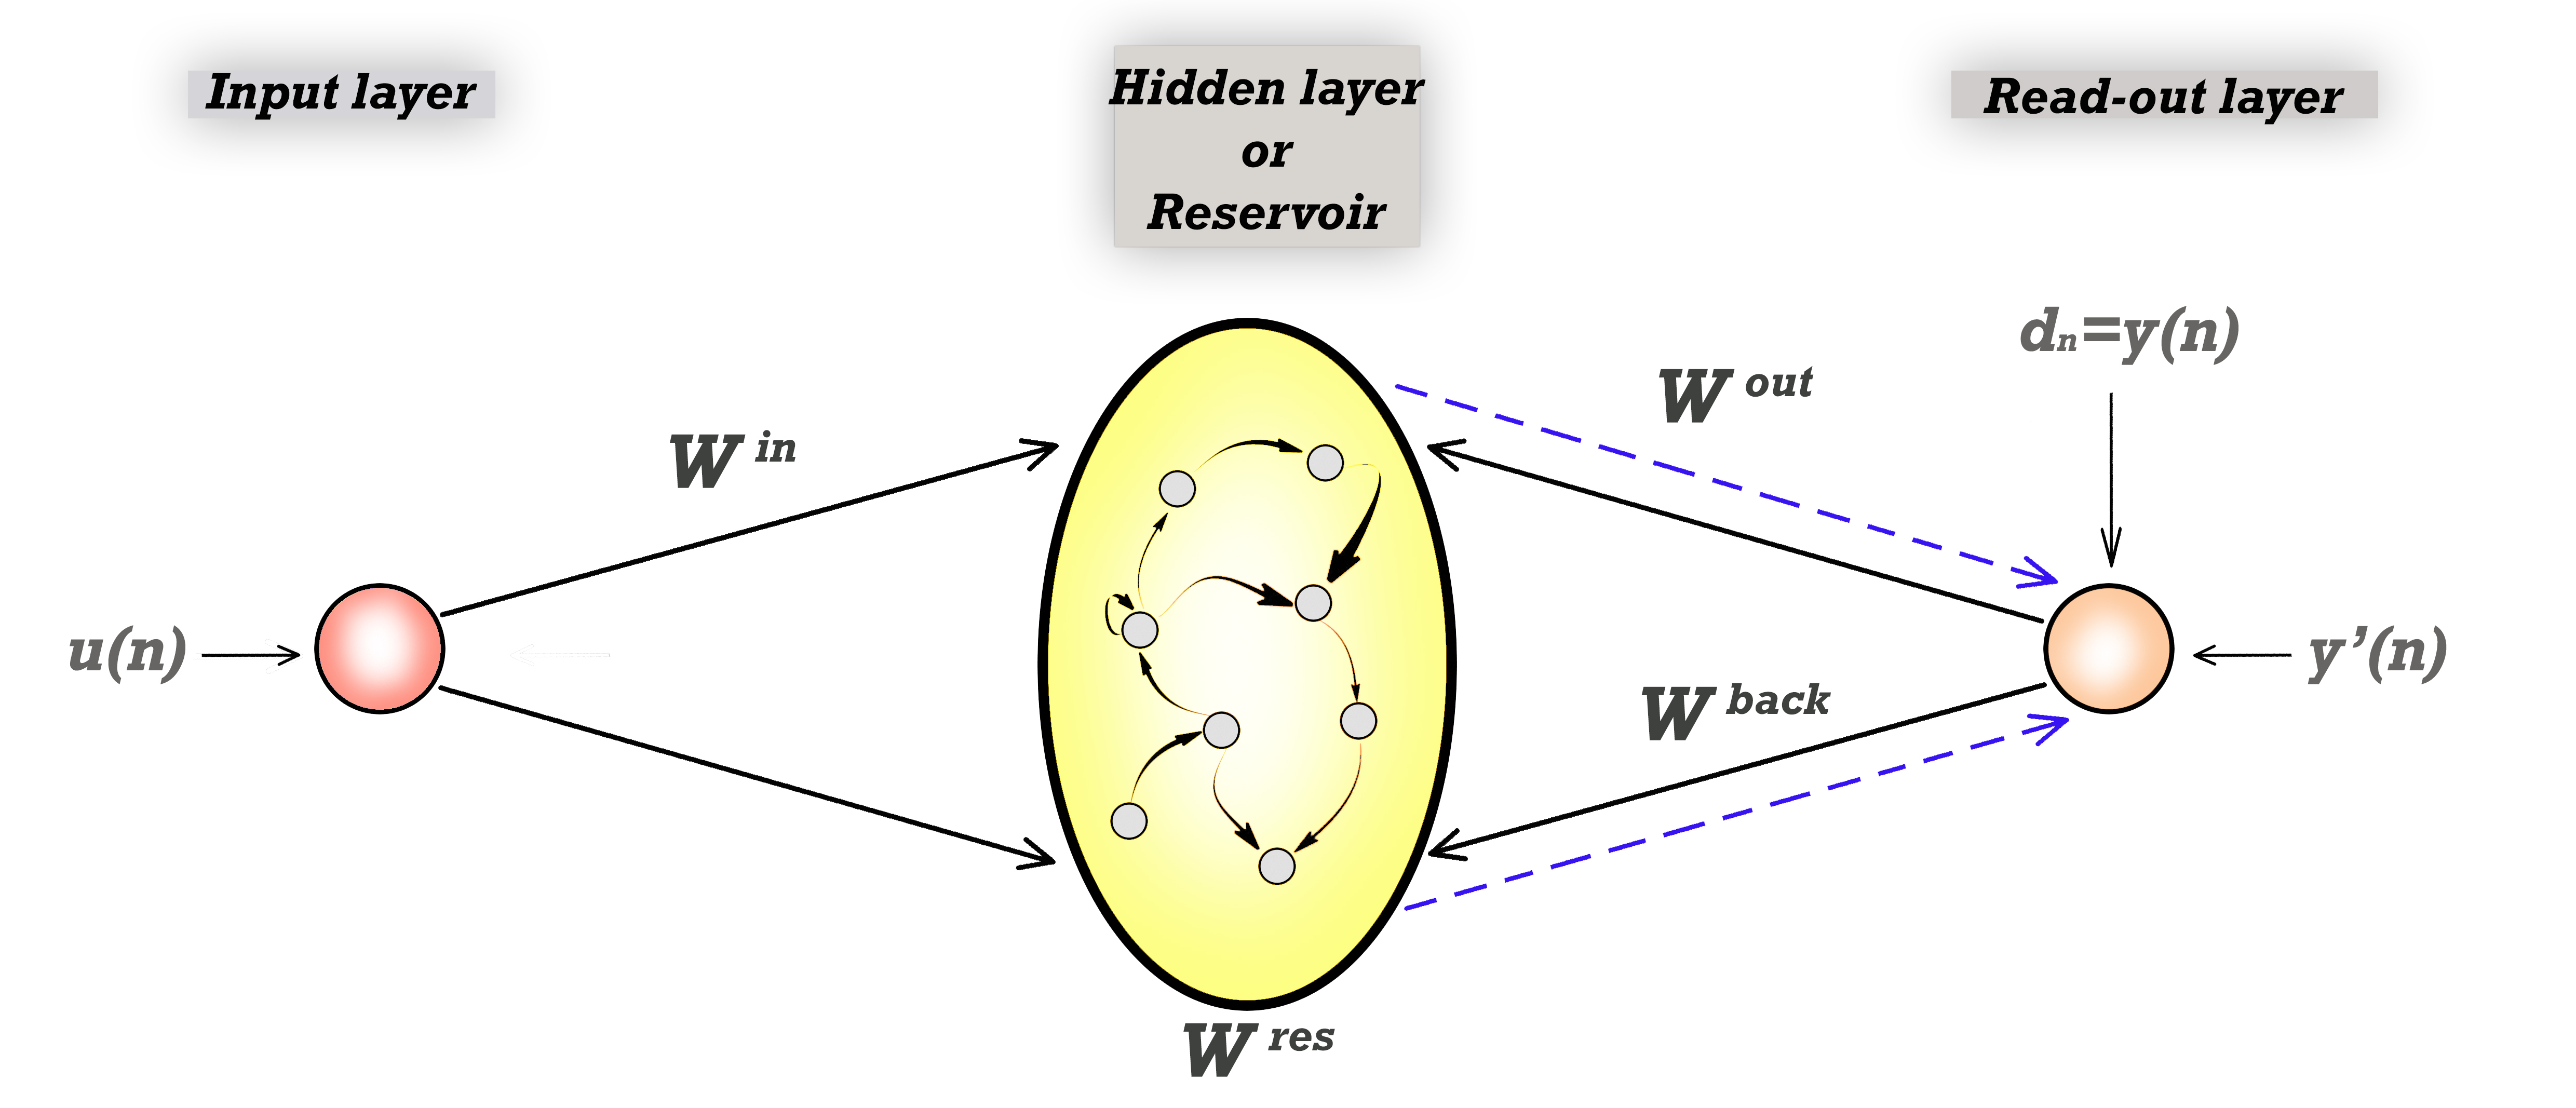
\includegraphics[width=0.8\linewidth]{esn_architecture}
\caption{\textbf{Architecture of classical ESN:} The reservoir is the recurrent neural network with N units and initialized with random connection. The reservoir is provided input from the input u(n) and y(n) from the input and output neurons  respectively. The input weights Win from input and Wback from output neurons are also randomly initialized and stays static during learning. The output  weight from reservoir to output unit is learned by the network.[ESN9]}
\label{fig:esn_arch}
\end{figure}

The Word2Vec model was trained using skip-gram negative sampling approach on a general purpose dataset (e.g. Wikipedia) and the domain specific dataset to learn the distributed embeddings for each word in the vocabulary(see section next). The reservoir of ESN, composed of leaky integrator neurons and sigmoids activations fuctions was randomly initilizied. A fixed fan-out of 10 and 2 is chosen for hidden-to-hidden and input-to-hidden connections respectively. In other words, each reservoir neuron is connected to 10 other reservoir neurons and each input neuron is connected to only 2 reservoir neurons. The input-to-hidden and hidden-to-hidden weights were generated sparse and randomly from a Gaussian distribution with mean 0 and variance 1. These weights once initialized are fixed and remains unchanged during training. The reservoir internal states for a given input sequence was accumulated across time which is then linearly combined with the desired output (thematic roles) using ridge regression to learn reservoir to readout weights. The reservoir internal states are simply the non-linear high dimensional expansion of input sequence[ref?]. Reservoir to readout weights are the only weights learned during training. The mathematical expressions for reservoir state updates and learning output weights are discussed in more details in section [ref]. The ridge regression was used rather than classical linear regression so as to avoid over-fitting and improve generalization capabilities, as it restricts the magnitude of readout weights[ref]. The learned readout weights can then later be used for generating coded meaning for the test sentences which were previously not seen by the model.

To ensure the objectivity of our findings we used two variants of the proposed models which were used to perform the experiments. Although both the variants are architecturally similar but varies in training objective and the evaluation metrics used evaluate the model performance. The number of units in input and output layer differs for each variation. Thus the input and output coding for ESN also differs depending on the training objective. The difference in variants is discussed in more details in next two subsection sections.

\subsection{Model Variant-1}

This variant of the model (see fig. \ref{fig:model_variant_1}) treats the thematic role assignment task as a prectition problem. The objective of the model variant is to predict the role of semantic words in a sentence with respect to a verb. To evaluate the performance of this model variant meaning error and sentence error metrics were used.(see section- Evaluation Metrics).

\begin{figure}[hbtp]
\centering
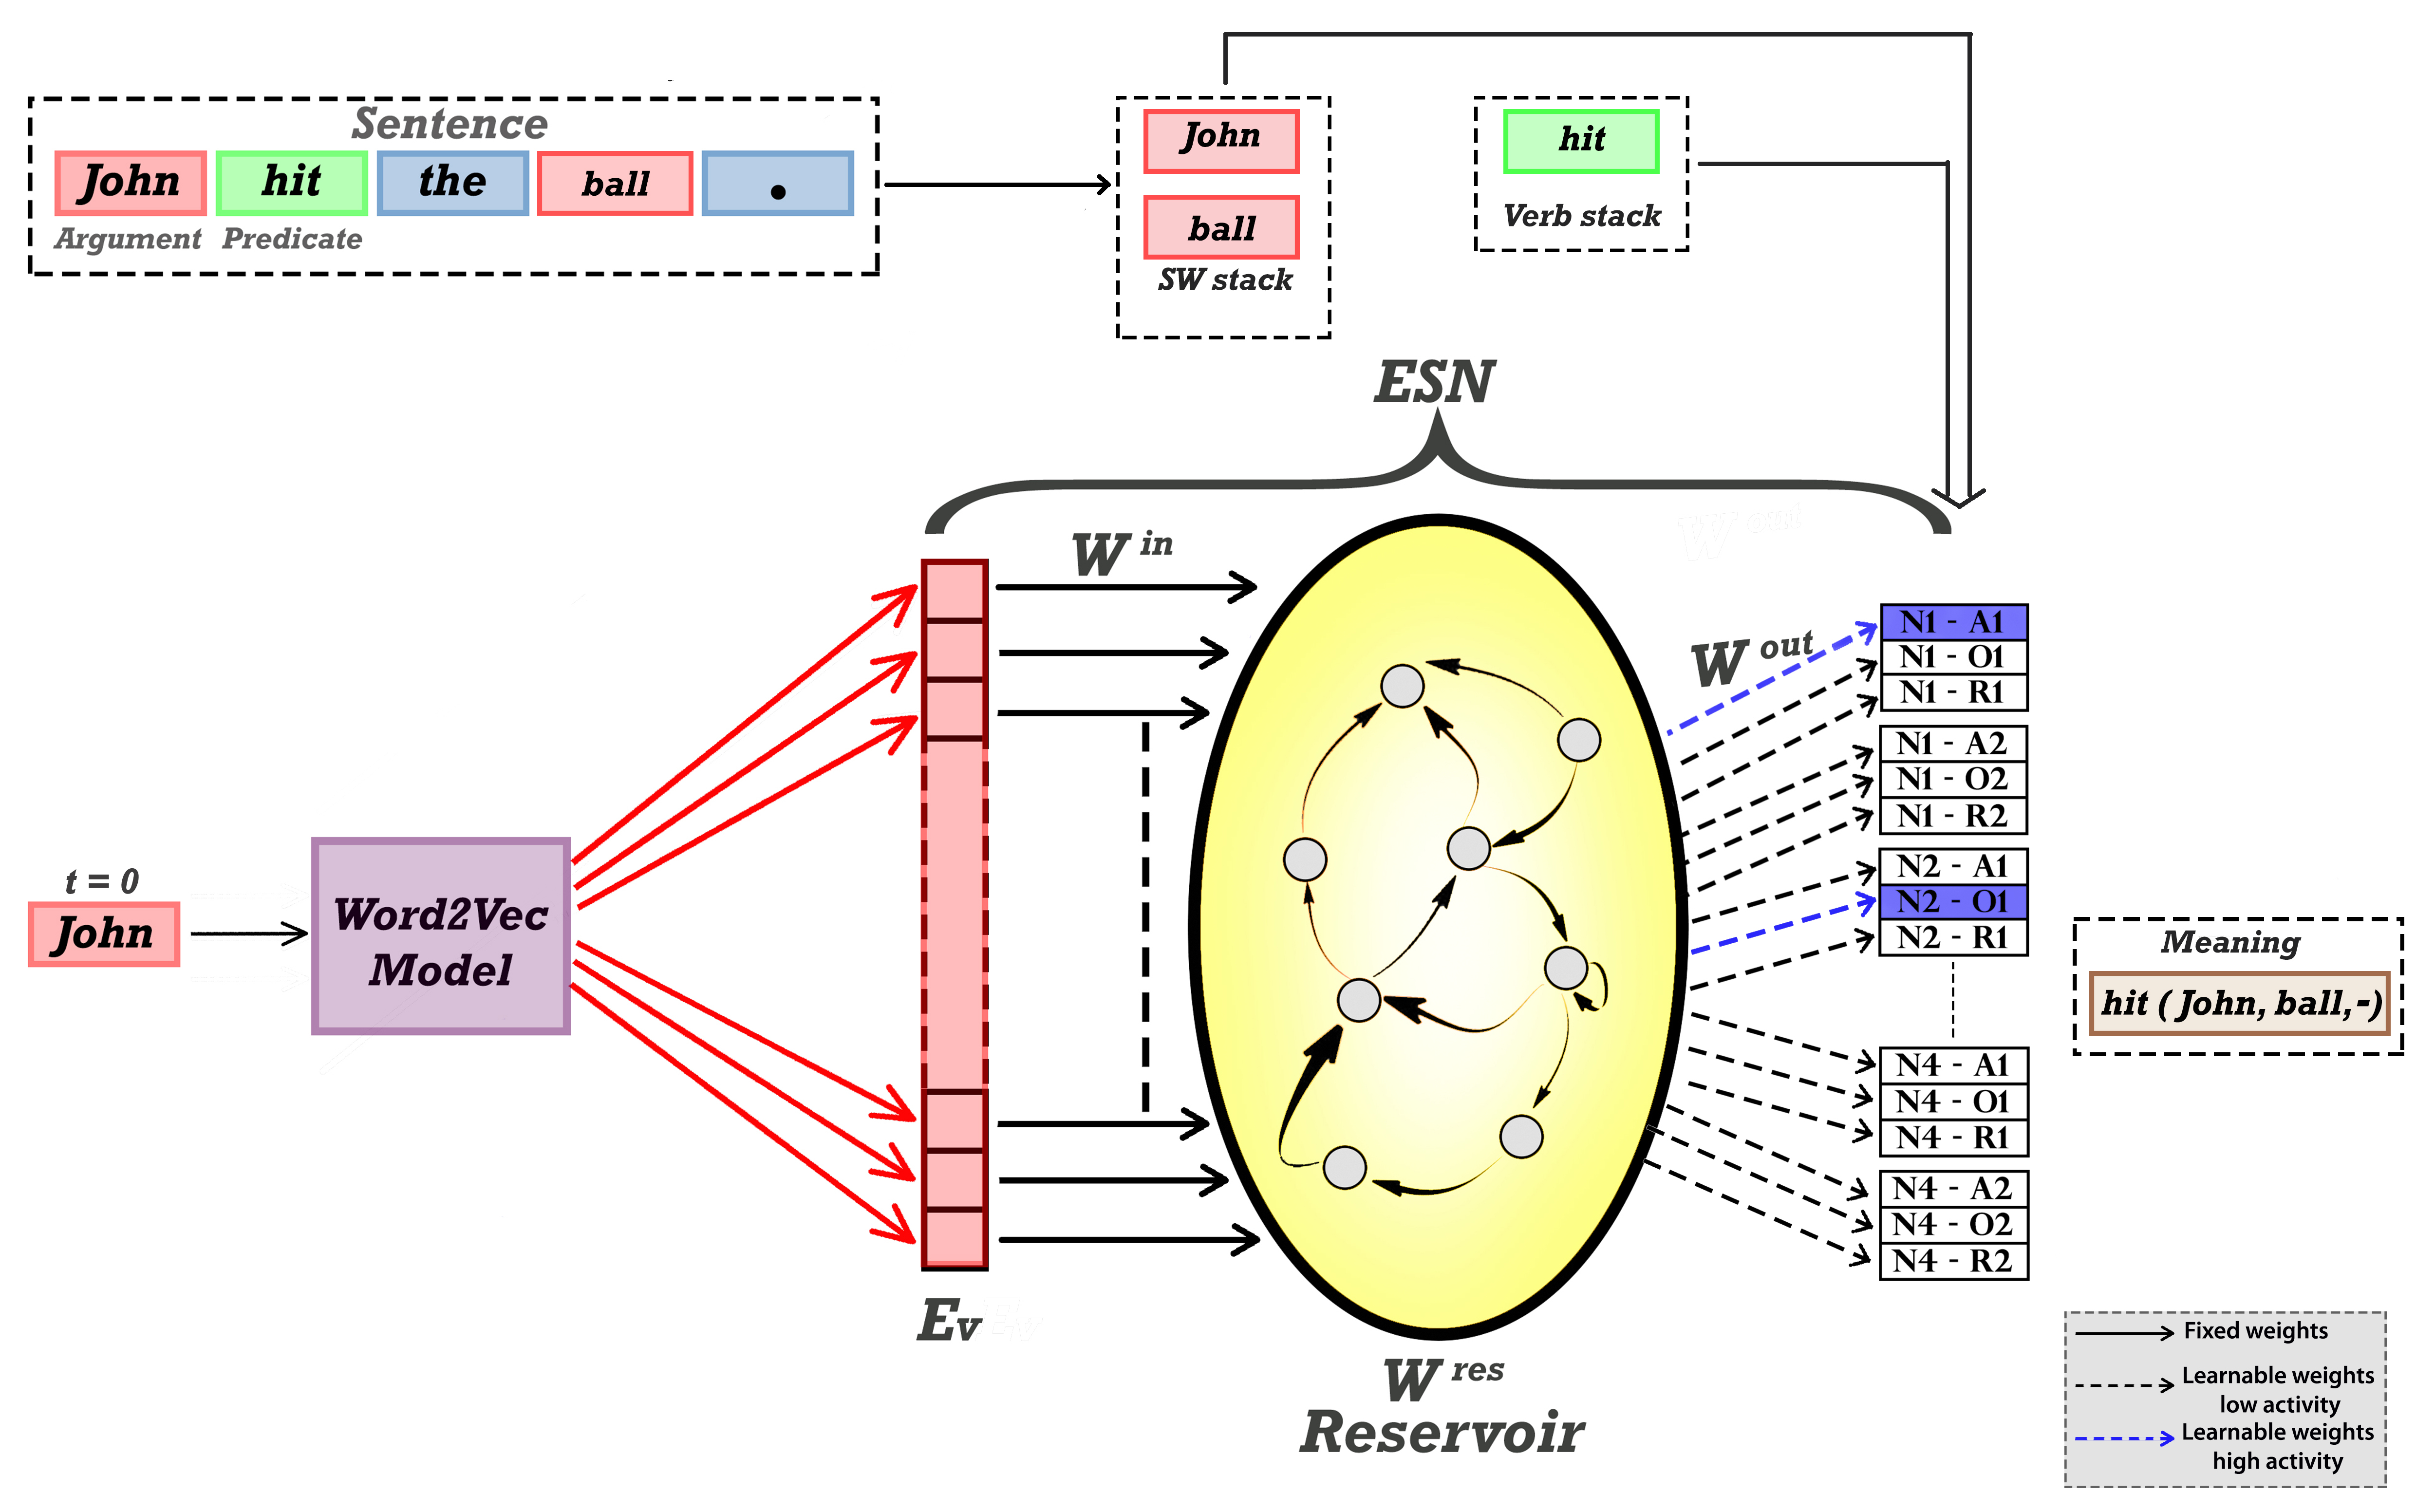
\includegraphics[width=0.8\linewidth]{model_variant_1}
\caption{\textbf{Word2Vec-ESN Model Variant-1:} The figure shows the processing of a sentence by the model variant at time step 1. Nouns and verbs (specified in orange and green respectively) are stored in a memory stack for interpretating coded meaning. The word 'John' is input to word2vec model which generate a word vector of $E_{v}$ dimensions. The output vector is then input to ESN for further processing. During training the readout units are presented with the coded meaning of the input sentence(i.e. N1-A1: Noun-1 is Agent of verb 1, N2-O1: Noun-2 is object of verb 2). In testing, the readout units codes the predicted meaning of input sentence. The meaning: hit(John,ball,--) is decoded by mapping the thematic roles predicted by readout neurons with nouns and verbs from memory stack. Adapted from \cite{xavier:2013:RT}} 
\label{fig:model_variant_1}
\end{figure}

The training sentences are presented to the model one at time, word-by-word across time. We initially prepare two memory stacks, one for storing nouns and one for storing verbs (see fig \ref{fig:model_variant_1}). Word2Vec model then receives the input word and generate the vector embedding of $E_{v}$ dimensions which is then input to the ESN. The input layer of ESN uses these distributed embeddings as input features for learning and predicting thematic roles of the sentences. Thus the size of input layer is same as the dimensionality of word vector i.e. $E_{v}$. The output of reservoir is accumulated for each time step during the presentation of a sentence. The reservoir states are reset before the presentation of the consequent sentence. The size of readout layer depends on the maximum number of semantic words (e.g. nouns and verbs) a sentence can have in the corpus. A noun can have one of the three possible roles: Agent, Object and Recipient, with respect to a verb. For example, if the sentences in the corpus have maximum of $N_{n}$ nouns and $N_{v}$ verbs then the readout size would be $N_{n} \times N_{v} \times {3}$  neurons; each output neuron encodes the thematic role of a semantic word (e.g. noun). The output neurons have an activation of 1 if corresponding thematic role is present for the sentence, -1 otherwise. The accumulated reservoir states are then linearly combined with readout activations to learn the reservoir-to-readout weights.

This model variant can be operated in two learning modes, so that it learns to extract the coded meaning of each noun with respect to a verb.

\begin{enumerate}
\setlength{\itemsep}{\smallskipamount}

\item \textbf{Sentence Continuous Learning Mode}: In this learning mode learning takes place from the beginning of the sentence till the end of sentence or in other words the teacher labels (coded meaning) for the sentece is made availabel to model from the onset of first word in sentence. Thus, the regression is applied with teacher labels from the onset of first word in the sentence. \label{eg:SCL}

\item \textbf{Sentence Final Learning Mode}: In this mode the learning takes places only at the end of the sentence. Hence, the teacher labels are only provided to the network at the end of sentence i.e. from last word of the sentence to the final period. \label{eg:SFL}

\end{enumerate} 

\subsubsection{Decoding Output}

As described earlier, coded meaning of sentence is defined as the description of thematic roles for all the semantic words (e.g. nouns,verbs etc.) in the sentence (see fig). As the readout neurons codes the thematic roles for individual semantic words, word level coded meaning were obtained in two steps. For every semantic word (e.g. noun) the readout activity is threshold at 0 and then the maximum of all the activations between 3 possible roles (i.e. Agent, Object, Recipient) is taken as the coded meaning of this semantic word. A semantic word is said to have incorrect coded meaning if the winning readout neurons is not the correct role of the semantic word. If there is no activation above threshold for a semantic word, then this semantic word is considered to have no coded meaning. The coded meaning of the sentence can then be interpreted from the the word level meaning by mapping the nouns and verbs from the memory stack created before giving the sentence to the model (see fig \ref{fig:model_variant_1}).

\subsubsection{Evaluation Metrics}

To evaluate the performance of this model variant two error measures were evaluated: the meaning error and the sentence error. Meaning error is the percentage of semantic words with incorrect coded meaning, whereas the Sentence error is the percentage of sentences having at least one semantic word with incorrect coded meaning [ref. xavier paper]. Both the error measure are related but there is no strict corelation between them. Sentence error is a more stricter measure than meaning error to evaluate model performance because a meaning error of $5\%$ cannot be used to estimate the sentence error, as these $5\%$ incorrect words can be from just one sentence or several sentences. 

For the analysis not all the readout neurons are considered i.e. if a sentence have only 2 semantic words then only readout neurons corresponding to these two semantic words were analyzed [ref.]. If there are more than one verb, in a sentence then each semantic word can have possible role with respect to each verb. Thus readout neurons corresponding to the mapping of semantic word and the verbs are used for analysis. For example in the sentence "John threw the ball and then he caught it". Each semantic word "John" and "ball" can have possible roles with verbs "threw" and "caught". So there are 4 possible output mappings for both the semantic words to their coded meaning. 

\subsection{Model Variant-2}

This variant of the model process the sentence differently from variant-1 and consider thematic role assignment task as a classification problem. The training objective is classify the words in the sentences to one of the roles namely Verb, Agent, Object, Recipient and XX (No-role) and maximize the the classification scores (i.e. F1-score, Precision and Recall- see section-) for each role. 

Training sentences are presented to the model sequentially, word by word. Two input features plays an important role in this model variant: argument and predicate, with argument describing the current word being processed and predicate describes the verb with respect to which argument is processed. So, if there are $N_{v}$ verbs in a sentence than the sentence is processed $N_{v}$ times. Each argument then takes a unique role for an argument-predicate pair. For example in the following sentence there are two predicates namely 'chased' and 'ate'. Thus this sentence will be processed twice and each argument will take a role for an argument-predicate pair.

\begin{table}[!htb]
\centering
\label{tab:argument-predicate}
\begin{tabular}{lccccccccc}
Arguments           & the & dog & that & chased & the & cat & ate & the & rat \\
Predicate('chased') & XX  & A   & XX   & V      & XX  & O   & XX  & XX  & XX  \\
Predicate('ate')    & XX  & A   & XX   & XX     & XX  & XX  & V   & XX  & O  
\end{tabular}
\end{table}

 At any time instant an argument and the predicate is input to the model where initially Word2vec model generates the distributed embeddings for both the input words. The generated word embeddings are concatenated and then taken by ESN as an input. Thus the size of ESN input layer is $2 \times E_{v}$ where the first $E_{v}$ neurons takes the vector representation of the argument and remaining $E_{v}$ neurons for the predicate. The reservoir internal states are collected for an input sequence over time which will be used later for regression with the desired output. The readout layer have 5 neurons each coding for a role. An output neuron have an activation 1 if the input argument have the corresponding role, -1 otherwise. The regression is performed with collected reservoir states and the readout activations to learn the reservoir-to-readout weights. Figure\ref{fig:model_variant_2} shows the processing of an example sentence by the model variant.

\begin{figure}[hbtp]
\centering
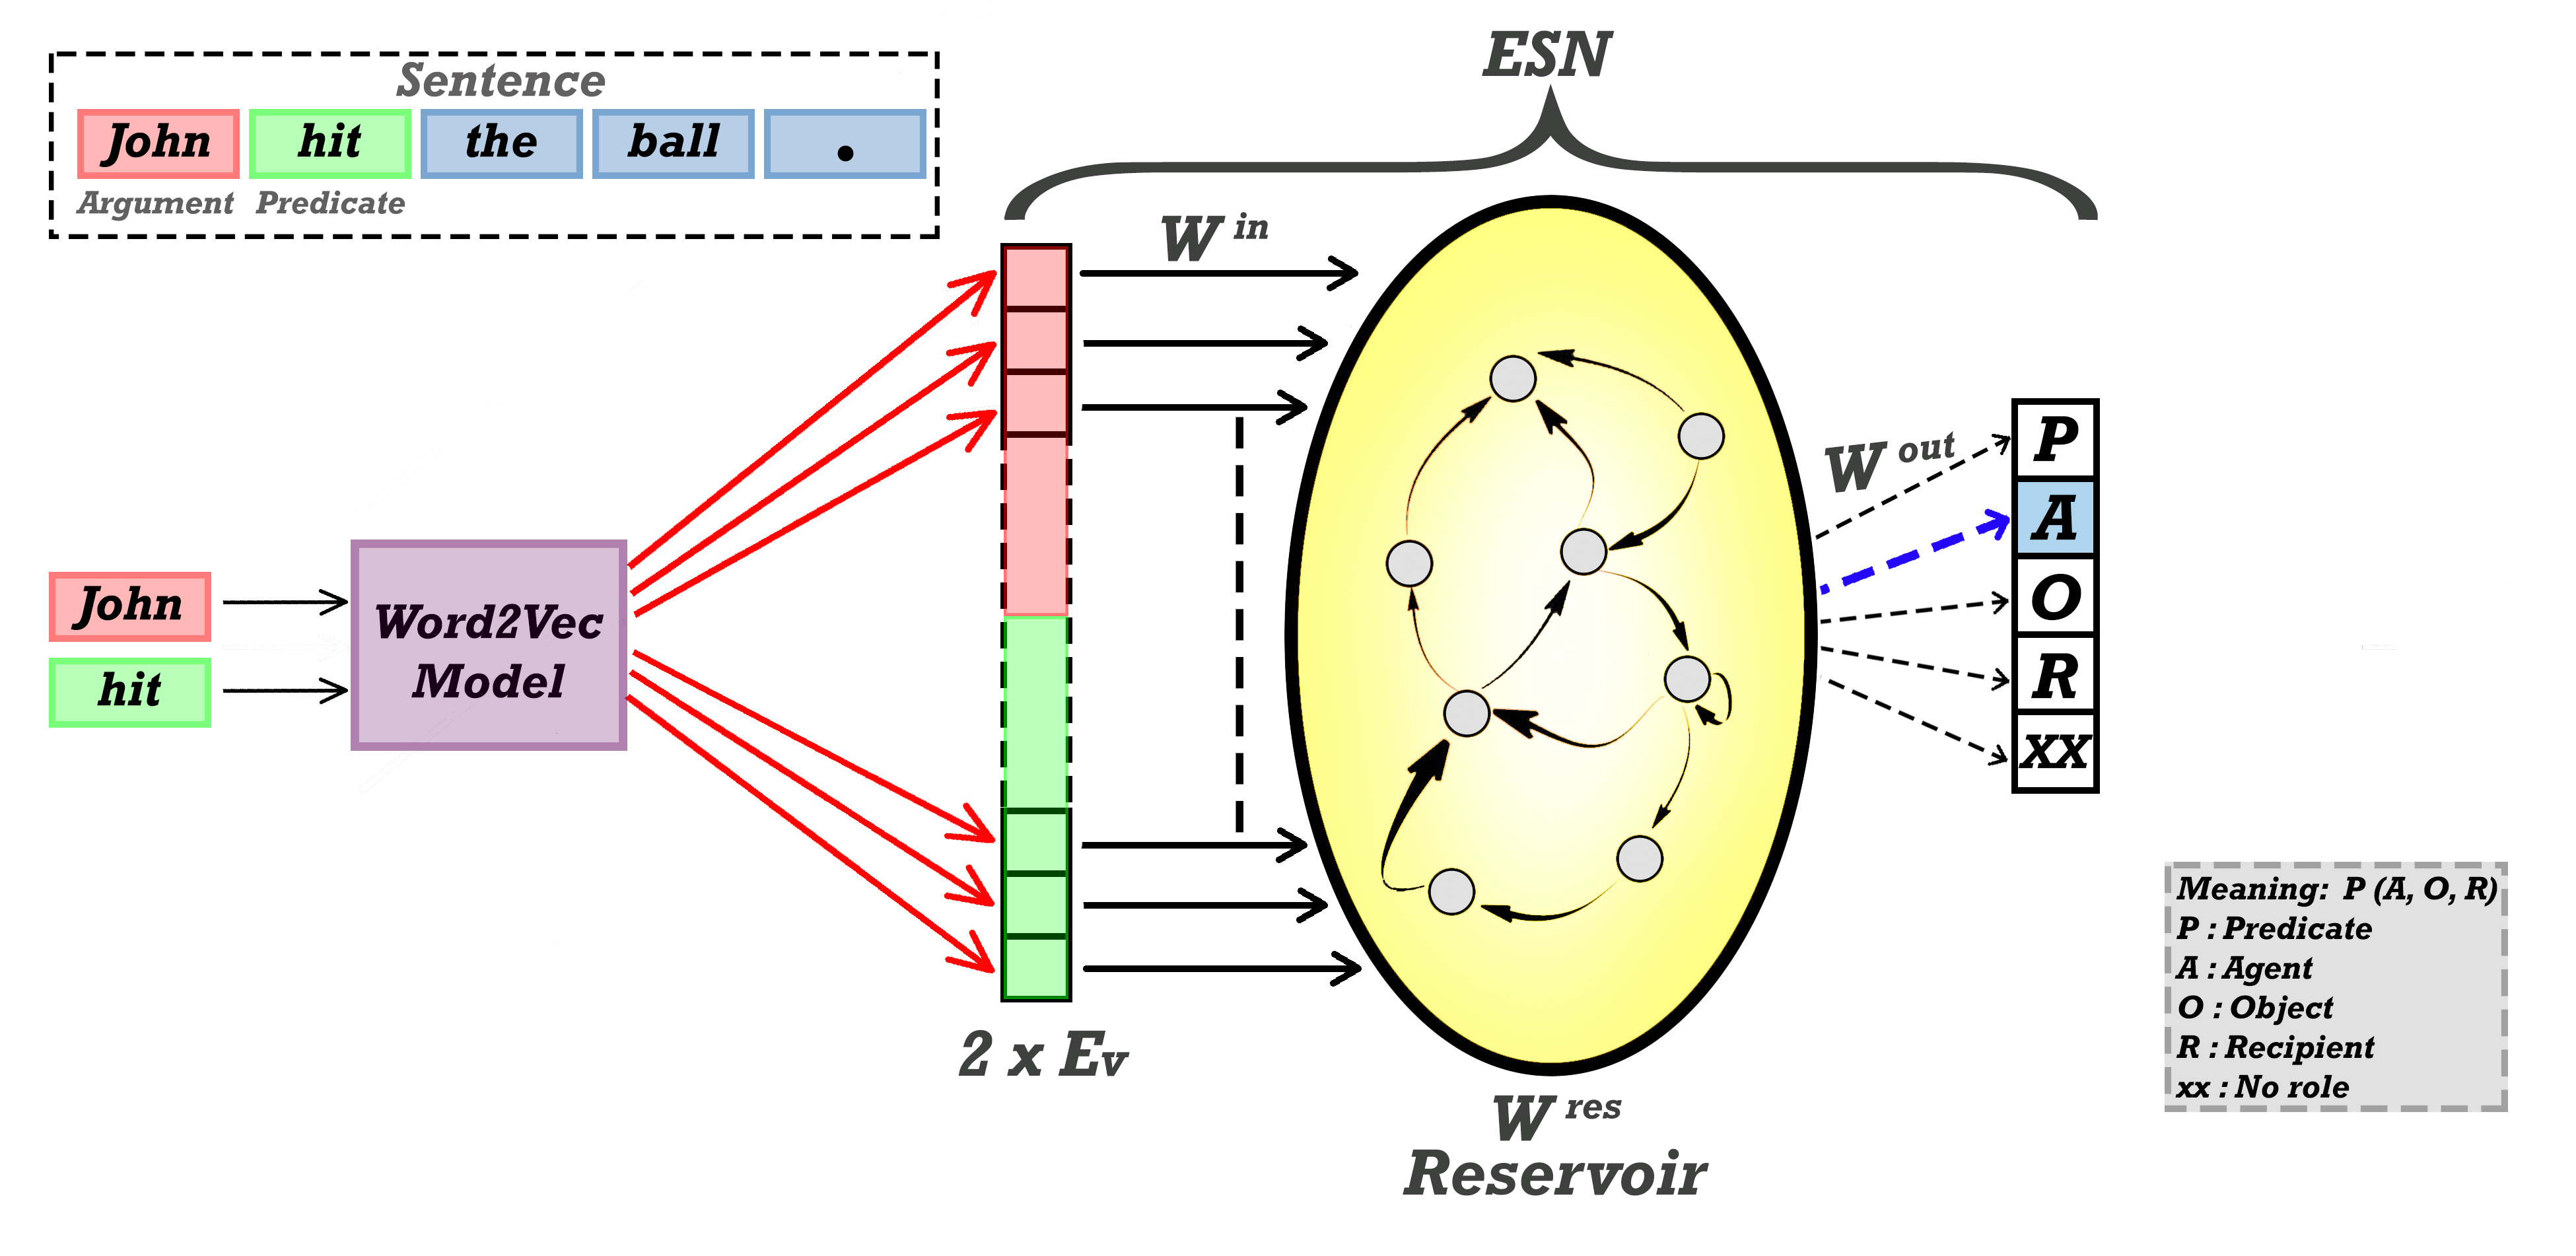
\includegraphics[width=0.8\linewidth]{model_variant_2}
\caption{\textbf{Word2Vec-ESN Model Variant-2:} 
The figure shows the process of a sentence in model variant-2 at time step 1. At any instant of time an argument (current word, marked in orange) and predicate (verb,marked in green) is input to the model. Word2Vec model generates the word vectors of $E_{v}$ dimensions which are then cocatenated to form a $2 \times E_{v}$ dimensions(shown in orange and green color). ESN takes the resultant vector for further processing. During learning, the readout neurons are presented with the role of input word (i.e. A (Agent)). The read-out weights (shown in dashed line) are learned during training. During testing the readout unit codes the role of input words, which are then accumulated and decoded to meaning \textit{hit(John,ball,--)} at the end of sentence. Inspired from \cite{xavier:2013:RT}
}
\label{fig:model_variant_2}
\end{figure}

\subsubsection{Decoding Output}



\subsubsection{Evaluation Metrics}

To analyze the performance of this model variant, the confusion matrix or contigiency table (Kohavi and Provost, 1998) was build and classification scores were calculated for all possible roles: Accuracy, Precision, Recall and F1-Score. The classification scores were then averaged, weighted by support (number of true samples for each roles), to get a single real numbered scores. Weighting the average score by support takes into account the role imbalance in the dataset. The same evaluation metrics was used for CoNLL-04 and CoNLL-05 Semantic Role Labelling task[ref.].

%draw confusion matrix from actual data

The confusion matrix describes the prediction made by the model. The rows of the matrix corresponds to the actual roles available in the dataset and the columns corresponds the predictions made by the model. The diagonal elements of this matrix represent the number of words for which the predicted role is equal to the true role,  whereas all the non-diagonal elements represents the number of word which were labelled incorrectly. As the values of diagonal elements of confusion matrix indicates number of correct predictions so higher the values of diagonal elements the better.

Using the confusion matrix accuracy can be calculated as ratio of number of correctly labelled words to total number of words (equation \ref{eqn:accuracy}). This meaures specifies how often the classifier is correct. 

\begin{equation}\label{eqn:accuracy}
Accuracy= \frac{\text{number of words correctly labelled}}{\text{total number of words}}
\end{equation}
 
However this measure can be distorting when the  dataset have words with large role imbalance as it gives high scores to models which just predict the most frequent class and cannot be used alone to evaluate the model performance[ref.]. In our dataset we have imbalanced roles as most of words have labels "XX" (No Role) compared to other roles. Thus we needed additional measures such as Precision, Recall and F1-score to evaluate the model. All these scores are reported as a value between 0 and 1. 

Precision is defined as ratio of True positive (TP) to False Positive(FP) and True Positive (equation \ref{eqn:precision}). It is the measure of the accuracy of a role provided that a specific role has been predicted. 

\begin{equation}\label{eqn:precision}
Precision= \frac{\text{True Positive}}{\text{True Positive + False Positive}}
\end{equation}

In the confusion matrix above, the precision for the role Agent(A) would be calculated as:

\[Precision(A) = \frac{TP_{A}}{(TP_{A}+E_{BA}+E_{CA})}\]

Recall is defined as the ratio of True Positive to True Positive and False Negative. It measure how good a model is labelling the correct roles. It is also called Sensitivity or True Positive Rate.

\begin{equation}\label{eqn:precision}
Recall= \frac{\text{True Positive}}{\text{True Positive + False Negative}}
\end{equation}

Recall for the role Agent, in above confusion matrix will be:
\[Precision(A) = \frac{TP_{A}}{(TP_{A}+E_{BA}+E_{CA})}\]

F1-Score is the harmonic mean of precision and recall. In other words, it represents the balance between the precision and recall and is calculated as:

\begin{equation}\label{eqn:precision}
F1= 2\times \frac{\text{Precision} \times{Recall }}{\text{Precision + Recall}}
\end{equation}

\section{Comparision of Model Variants}




\section{Dataset and pre-processing}

\subsection{Corpus For TRA Task}

For the experiments we used corpus of 462 sentence and 90582 sentences. The same corpus was used in thematic role assignment in [ref?]. The sentence in corpus-462 was generated using a context-free-grammer for English language. Each sentence in this corpus can have verbs which can take 1, 2, or 3 arguments. For example sentences, “The man jump” , “He cut an Apple” , “John gives ball to Marie” have 1 , 2 and 3 arguments respectively)[ref]. The sentences in the corpus have a maximum of four nouns and two verbs. A maximum of 1 relative clause is present in the sentences; verb in the relative clause could take 1 or 2 arguments (i.e., without recipient). For e.g. “The dog that bit the cat chased the boy”. The coded meaning for each sentence is described in order of Predicate, Agent, Object and Recipient. 

	Corpus-90582 consist 90582 sentences along with the coded meaning of each sentence. This corpus is redundant; multiple sentences with different grammatical structure have the same coded meaning (see fig). In total there were only 2043 distinct coded meanings[ref] . This corpus also have an additional property that along with complete coded meanings for sentences it also have incomplete meanings. For e.g. the sentence “The Ball was given to the Man” have no Agent, and Thus the meaning of the sentence is give(-,ball,man) [ref]. The corpus also contains 5268 pair and 184 triplets of ambiguous sentences i.e., 10536 and 553 sentences respectively. Thus in total there were 12.24 \% (i.e., $ 5268 \times 2+184*3=11088 $) of ambiguous sentences which have the similar grammatical structure but different coded meaning. 
Both the corpus-462 and corpus-90582 have the constructions in form:

walk giraffe <o> AP </o> ; the giraffe walk -s . \# ['the', 'X', 'X', '-s', '.']
cut beaver fish , kiss fish girl <o> APO , APO </o> ; the beaver cut -s the fish that kiss -s the girl . \# ['the', 'X', 'X', '-s', 'the', 'X', 'that', 'X', '-s', 'the', 'X', '.']

Each construction in the corpus is divided into four parts. The first part describes the meaning of sentence using Semantic words(or Open class words) in order of Predicate, Agent, Object, Recipient. The second part describes the order of thematic roles as appears in the raw sentence. The third part is the raw sentence with verb inflections and the fourth part is the abstract grammatical construction of sentence with Semantic words removed.

	We preprocessed these constructions, to obtain the raw sentences without verb inflections. Firstly all the words are lower cased and then the verbs with inflection is modified and replaced by conjugated verb. The verb conjugation to be used depends on the inflections the verb has. For e.g “The giraffe walk -s” has been changed to “The giraffe walks”. The reason replacing verb and its inflections with verb conjugation is that we have distributed word representation which captures this syntactic relations e.g walks-walk=talks-talk. We also added additional token <start> at the beginning of sentence and <end> token at end to mark the beginning and end of a sentence.
  
\subsection{Corpus For Training Word2Vec Model}

To train the word2vec model, we used wikipedia corpus to obtain the word embedding of words.
% Give properties of dataset here
 We chose to use Wikipedia data because we need to have vector representation of words and more words you have the better the vector representation. The Word2Vec model do not give good vector representation for words when trained over a small corpus thus a general purpose data set with billions of words is required to have good word embeddings. Once the vector representation of Wikipedia data is obtained the model can be trained further on any our domain specific dataset (corpus-462 and corpus-90582) with more bias toward (by repetition of dataset during training) domain specific dataset to update the previously learned vector representations. 

\section{Word Embeddings}

To get the vector representation of words we first trained a word2vec model on Wikipedia dataset. For training we used Word2vec skip-gram negative sampling (see Chapter 2 for more details) approach to obtain the word embeddings as it is claimed to produce better representation as compared to CBOW approach and is faster to train[ref?]. We used the hidden layer of with 50 units (desired dimensions of word embedding), and  a context window of length +-5. The negative sampling size is chosen to be 5 i.e. 5 noise words are chosen randomly from the vocabulary which does not appear in the context of the current input word. We ignored all the words which appears less than 5 times in the corpus. For network weight update stochastic gradient, the initial learning rate was set to be $\alpha=0.025$, which drops to $min_alpha=0.0001$ linearly as training progresses. 

The word embeddings obtained from training on Wikipedia dataset are good enough to capture the semantic relationship for e.g. $vec(Paris)-vec(France)+vec(Germany)\approx vec(Berlin)$. But the limitation was that once the vocabulary is created from the wikipedia dataset, it was not possible add new words in the vocabulary. However there is a possibility that some of the domain specific corpus is used to train the model in extension to wikipedia corpus some words may not be present in vocabulary generated while training on wikipedia corpus. Thus we needed to update the vocabulary of the model if the word is not present in order to facilitate online training of Word2Vec model. Unfortunately neither C++ API[ref?] nor Gensim python API[ref?] implementation of Word2Vec supports vocabulary update if once created. So, adapting the idea suggested by [ref Radim and Dr, Rutu Mulkar-Mehta], we implemented the online training of word2vec by extending Gensim API. The new words not present in existing vocabulary is added and initialized with some random weights, which can then be trained in usual manner to have vector embeddings. Although now the vocabulary can be updated in online manner but the vector embedding of newly added word have poor quality if its count in new corpus is few. This can be improved by repetition of new dataset several times before training the model [ref? Google group gensim].

So now when we have an online version of training word2vec model, we extend word2vec model by resuming training on corpus-462 and corpus-90582. While updating the model on new dataset we do not disregard any words irrespective of the count, so that we have vector embeddings of all the words in our corpus. Once trained the vector embeddings are normalized using L-2 norm before using them for further use. 


\cleardoublepage

\chapter{Experiments and Results}\label{results}

In chapter we describe the experiments performed with the Word2Vec-ESN model and the variant proposed in the previous chapter. The results obtained by the Word2Vec-ESN model, using word embeddings, are compared with $\theta RARes $ model which uses sentence in grammatical form by replacing semantic word with 'SW' token and localist representation of words.

\section{Input and Ouput Coding}

\paragraph{Word2Vec-ESN model:} A raw sentence is presented to the model, where each word in the sentence is processed across time by both word2vec model and ESN. The word2vec model outputs the $E_{v}=50$ dimension word embedding which is then used as input for ESN. Thus input layer have 50 neurons. For the experiment with corpus-462 we used a reservoir of $1000$ leaky integrator neurons with \textit{tanh} activation fuction. For the output coding the topologically modified but equivalent representation is used \cite{xavier:2013:RT}. Thus, the readout layer contains 24 $(4 \times 3 \times 2)$ neurons as the corpus contains sentences having maximum of 4 nouns each having 3 possible roles (Agent, Object and Recipient) with respect to a maximum of 2 verbs. Output neuron have an activation 1 if the role is present in the sentence, -1 otherwise. Whereas when using corpus-90582 for training the number of neurons in reservoir were raised to 5000 and also the  readout neurons are increased to 30 $(5 \times 3 \times 2)$ as there were maximum of 5 nouns in the sentences of this corpus.

\paragraph{Word2Vec-ESN model variant:} In the Word2Vec-ESN model variant a raw sentence is presented to the model, where each word (argument) along with the verb (Predicate) with respect to which the word is currently processed, is input to the model across time(see section \ref{sec:model_variant}). A sentence is processed as many time as there are verbs in the sentence. The word2vec model firstly takes this argument-predicate pair as an input and outputs a vector of $E_{v}=2 \times 50$ dimension, which is then used as an input to ESN. Thus input layer thus have 100 neurons where first 50 neurons encodes the vector representation of the word and remaining 50 neurons codes for the verb with respect to which word is processed. The reservoir of size 1000, 3000 is used for corpus-462 and corpus-90582 respectively. Unlike the model variant-1, the size of readout neurons always remains the same and contains 5 neurons each coding for a role: Predicate (P), Agent(A), Object(O), Recipient(R) and No Role(XX). Readout neuron of ESN have an activation 1 if the input word-verb (argument-predicate) pair have the corresponding role, -1 otherwise.

\section{Experiments}

\subsection{Experiment-1: Learning thematic roles}

In order to determine the model capability for predicting thematic roles of the sentences using word2vec embeddings for words, we first did the experiment using 26 sentences(sentence 15 to 40, in corpus-45) from corpus-45. The chosen sentences have distinct surface form (e.g. active, passive, dative-passive) and grammatical structure. This also include the sentences with single verb or double verb relative surface form [ref?]. Both the model variants(see section-?) learned the sentences without any error when trained and tested on all the sentences. To test the performance and generalization capabilities of model on untrained sentences, we performed a leave-one-out cross validation, where a model is trained on 25 sentences out of 26 and tested on remaining 1 sentence.

\paragraph{Model Variant-1:} The model variant-1 with a reservoir of size 1000 units the model yielded [?] meaning error and [?] sentence error in sentence continuous learning mode and [?] meaning error and [?] sentence error in Sentence final learning mode. The results were averaged over 10 reservoir instances. For Continuous learning model the spectral radius(SR), input scaling (IS) and leak rate($\alpha$) were identified as $SR=[?], IS=[?], \alpha=[?]$.` Whereas for Sentence final learning mode the $SR=?, IS=?, \alpha=?$. The ESN parameters for which the optimized results are identified are found by exploration of parameter space. As one may note that difference in training and test error for both meaning and sentence error is large. This indicates the model is overfitting on the dataset. However, it is not surprisring because the dataset contains limited examples, which constrained model to generalize well. As this experiments remains a toy demonstration we will explore the generalization capabilty of the model in section \ref{exp-2} .

\paragraph{Model Variant-2:} The model Variant-2, on the other hand, with a reservoir of size 600 neurons, produced the classification scores [write score here] during cross-validation. 

\subsection{Experiment-2: Generalization Capabilities} \label{exp-2}

In the previous experiment we demonstrated the performance of the model with the limited set of sentences where the results suggested that the model is probably overfitting and not generalizing on the unseen sentences. So in order to test the generalization capability of the model, we examined the model's behaviour with an extended corpus of 462 sentences (see corpus-462 in \ref{datasets}) using 10-fold cross validation. Corpus-462 with 462 sentences was randomly split into 10 equally sized subsets(i.e. each subset with $\approx$ 46 sentences). The model was trained on sentences from 9 subsets and then tested on remaining one subset. This process was repeated 10 times such that the model is trained and tested on all the subsets atleast once. 

\paragraph{Word2Vec-ESN:} We initially trained and tested the model with reservoir of 1000 neurons on all the 462 sentences. The model learned the full corpus-462 with $0.54\%$ meaning error and $1.51\%$ sentence error in SCL mode and $0.14\%$ meaning error and $0.43\%$ sentence error in SFL mode. Using the 10-fold cross validation, the model generalized to $7.82\% (\pm 1.59\%) $ meaning error and $20.65\% (\pm 2.79\%)$ sentence error in SCL mode with spectral radius (SR), input scaling (IS) and leak rate(LR) of $2.4$, $2.5$ and $0.07$ respectively. Whereas in the SFL mode with $SR = 2.2$, $IS = 2.3$ and $LR = 0.13$, the optimal meaning and sentence error were observed as $8.68\% (\pm 1.26\%)$ and $23.69\% (\pm 1.17\%)$ respectively. The optimal parameters for both the learning models (SCL and SFL) were identified using grid search over the parameter space.

We compared the performance of Word2Vec-ESN model with $\theta RARes$ model which takes the sentences in grammatical form and words are represented in localist fashion. As illustrated in table \ref{tab:corpus-462_errors}, during testing, we observed an improvement of $11.48 \%$ sentence error in SCL mode with Word2Vec-ESN model whereas meaning error remained almost equivalent in both the models. In SFL mode, using Word2Vec-ESN model, both meaning and sentence errors dropped nearly by $1 \%$. One can also notice that with Word2Vec-ESN model, the performance gain in more in SCL mode as compared to SFL mode. The reason is that the word-embeddings in word2vec model are learned from the context words and thus word vector encapsulates the information about neighbouring words.  

%NOTE: 08/09/2016 results are copied after the simulation and are final, no need to change.
\begin{table}
\centering
\begin{threeparttable}
\caption{Mean and standard deviation of meaning and sentence error on train and test set of coprus-462 in different learning modes.}
\label{tab:corpus-462_errors}
\rowcolors{2}{white}{gray!25}
\begin{tabularx}{\textwidth}{@{}llYYYY@{}}
  \toprule
  &  & \multicolumn{2}{c}{Word2Vec-ESN} & \multicolumn{2}{c}{$\theta RARes$} \\
  \cmidrule(lr){3-4}   \cmidrule(lr){5-6}
  \hiderowcolors   
  
  						& 		& ME 	& SE 			& ME 	& SE 		\\
  \midrule
  \showrowcolors
  \textbf{SCL\ train} 	& mean 	& 0.541 & 1.515 	 	& 0.123 & 1.207 	\\
   			    		& std 	& 0.000 & 0.000 	 	& 0.029 & 0.297 	\\
   			    		
  \textbf{SCL\ test} 	& mean  & 7.826 & 20.652 	 	& 7.433 & 32.130 	\\
  			   			& std  	& 1.598 & 2.792 	  	& 0.534 & 1.353 	\\
  			   			
  \textbf{SFL\ train} 	& mean 	& 0.144 & 0.432 	 	& 0.000 & 0.000 	\\
  				 		& std 	& 0.000 & 0.000 	 	& 0.000 & 0.000 	\\
  				 		
  \textbf{SFL\ test}	& mean  & 8.686 & 23.695 	 	& 9.178 & 24.370 	 \\
  			  			& std 	& 1.265 & 1.170		  	& 0.574 & 1.192 	  \\
  \bottomrule
\end{tabularx}
\begin{tablenotes}
\small
\item 
Meaning (ME) and Sentence error (SE) in different learning modes with Word2Vec-ESN model using distributed word embeddings and $\theta RARes$ \cite{xavier:2013:RT} model which uses grammatical form and localist representation of words of sentences. The errors are given in percentage. SFL:Sentence Continuous learning; SFL: Sentence Final Learning; std: Standard Deviations. Simulations were done with reservoir of 1000 neurons.
\end{tablenotes}
\end{threeparttable}
\end{table}
	
\paragraph{Word2Vec-ESN Variant:} The word2vec-ESN model variant with a reservoir of size 1000 neurons when trained and tested on all 462 sentences of corpus-462, learned to label the word in the sentences with an Accuracy(Ac), Precision(Pr), Recall(Re) and F1-Score(F1) of $97.38\%$,  $97.48\%$, $92.28\%$, $94.64\%$ respectively. When the model variant was tested using 10-fold cross validation we got Ac = $97.18\% (\pm 0.11\%)$, Pr = $96.86\% (\pm 0.49\%)$, Re = $91.93\% (\pm 0.23\%)$ and F1 = $94.16\%(\pm 0.26\%)$ with $IS=1.15, SR=0.7, LR=0.1$. The marginal difference between the training and cross validation scores indicates that the model variant is generalizing well even on untrained data and is not overfitting. The precision, recall and f1-score for individual role is listed in table \ref{tab:classsification-scores-21}. 

\begin{table}
\centering
\begin{threeparttable}
\caption{Training and testing classification scores for individual roles when using Word2Vec-ESN model variant.}
\label{tab:classsification-scores-21}
\rowcolors{2}{gray!25}{white}
\begin{tabularx}{\textwidth}{@{}llYYYYYYY@{}}
\hiderowcolors
\toprule
  &  & \multicolumn{3}{c}{word2vec vectors} & \multicolumn{3}{c}{GF \& localist vectors}& \\  
\cmidrule(lr){3-5}   \cmidrule(lr){6-8}
   
Role 				& 		& Pr   & Re  & F1 		& Pr  &  Re & F1 		&  Support  \\
\showrowcolors
\midrule
               
\textbf{Agent}		&test 	& 0.92 & 0.79 & 0.85 	& 0.66 & 0.62 & 0.64	& 888 \\
					&train  & 0.94 & 0.80 & 0.86 	& 0.71 & 0.68 & 0.69	& 892 \\
\textbf{Object}		&test 	& 0.95 & 0.81 & 0.88 	& 0.61 & 0.65 & 0.63	& 791 \\
					&train  & 0.96 & 0.81 & 0.88 	& 0.67 & 0.69 & 0.68	& 794 \\
\textbf{Recipient}	&test 	& 1.00 & 1.00 & 1.00 	& 0.69 & 0.96 & 0.80	& 383 \\
					&train  & 1.00 & 1.00 & 1.00 	& 0.70 & 0.97 & 0.81	& 384 \\
\textbf{Predicate}	&test	& 1.00 & 1.00 & 1.00 	& 0.96 & 0.92 & 0.94	& 888 \\
					&train  & 1.00 & 1.00 & 1.00 	& 0.98 & 0.94 & 0.96	& 892 \\
\textbf{No Role}	&test 	& 0.97 & 1.00 & 0.99 	& 0.97 & 0.96 & 0.97	& 9785 \\
					&train  & 0.97 & 1.00 & 0.99 	& 0.98 & 0.97 & 0.97	& 9823 \\
\bottomrule
\end{tabularx}
\begin{tablenotes}
\small
\item Comparision of training and cross validation scores for each output roles predicted by the model. Support for each role: actual number of instance, is also shown in last column. Simulation were done using 1000 reservoir neurons and parameters: SR = 0.7, IS = 1.15, LR = 0.1.
\end{tablenotes}
\end{threeparttable}
\end{table}

We also performed the simulations using Word2Vec-ESN model variant with grammatical form of sentences with localist word representation. The model produced Pr = $80.60 \%$, Re = $84.90 \%$, F1 = $82.31 \%$ during training and Pr = $78.04 \%$, Re = $82.23 \%$, F1 = $79.68 \%$ during cross-validation. 

% analyse table and confusion matrix
[Confusion matrix to be analyzed]

\begin{figure}[hbtp]
\centering
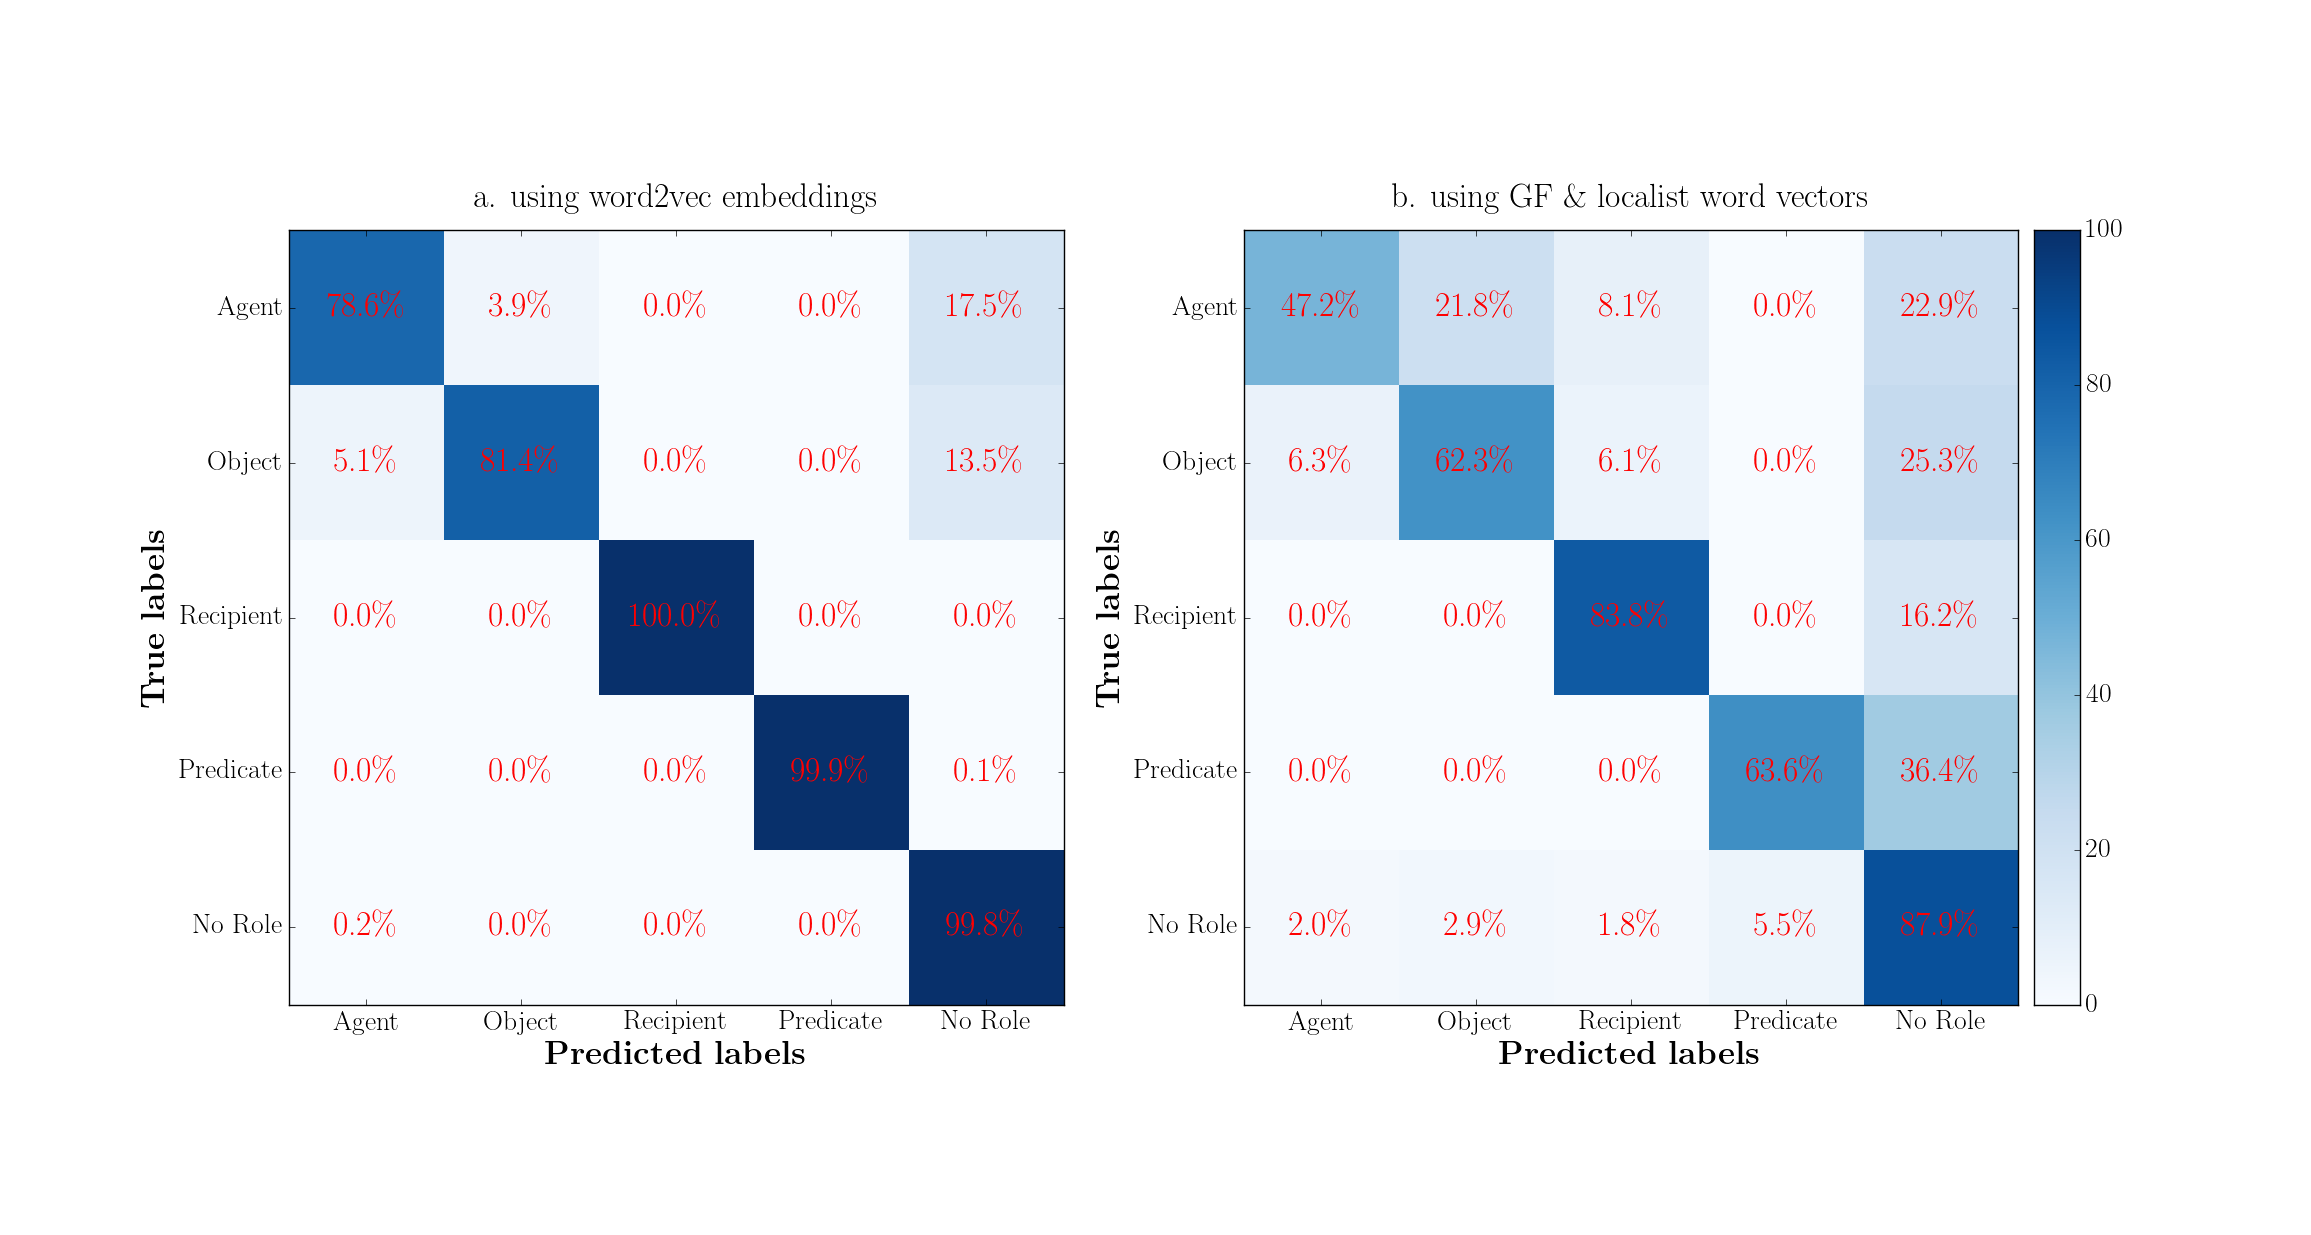
\includegraphics[width=1.0\linewidth]{confusion_matrix}
\caption[Normalized confusion matrix on corpus 462 with Word2Vec-ESN model variant] {\textbf{Normalized confusion matrix with Word2Vec-ESN model variant:} The confusion matrix with true roles (in rows) and predicted roles (in columns). The top-left to bottom-right diagonal shows the percentage of words whose roles are predicted correctly. Everything other than this diagonal represents the incorrect prediction of roles. Model identified almost all words labelled as Recipient , Predicate and No Role and made some errors in predicting role Agent and Object. The results were obtained with reservoir of 1000 neurons and 10 fold-cross validation.}
\label{fig:confusion_matrix}
\end{figure}


\subsection{Experiment-3: Effect of Corpus structure} 

Recall that the sentences in the corpus-462 was created based on context free grammer. Thus the sentences in the corpus contains inherent grammatical structure. The model is thus possibly utilizing the underlying grammatical structure to some extend for learning and generalizing. To test this hypothesis and to demonstrate that the model is not generalizing on any other inconsitent regularity in the corpus, we removed the inherent grammatical structure from the sentence in the corpus by randomizing the word orders within the sentences \cite{xavier:2013:RT}. Such a test will also help us to have insight on what the model is actually learning and whether the model is overfitting or not. The situation of overfitting typically occurs when the corpus size is significantally less than the number of trainable parameters \cite{xavier:2013:RT}. The Word2Vec-ESN model with reservoir of size 1000 neurons and 42 readout neurons have 42000 $(42 \times 1000)$ trainable parameters, whereas the model variant with reservoir size $1000$ and $5$ readout neuron the trainable parameters are 5000 $(5 \times 600)$. In both the case the number of trainable parameters are significantally greater than our corpus size (i.e. 462 sentence). This is thus a possible situation of overfitting.

We presented the corpus with the scrambled sentences(i.e. in absence of any grammatical structure) to both Word2Vec-ESN model and its variant and performed a 10 fold cross-validation. The cross validation errors obtained in the previous experiment on the corpus with inherent grammatical structure can then be compared with the cross validation error obtained while using scrambled corpus. If the model is not overfitting and learning from the grammatical structure then the model should generalize better for the corpus with unscrambled sentences (i.e. in presence of grammatical structure). However in case of overfitting the generalization effect should not vary much both in presence and absence of grammatical structure in the corpus.

As illustrated in Table.[no], we observed that [analysis to follow....]

\begin{table}
\centering
\begin{threeparttable}
\caption{Mean and standard deviation of meaning and sentence error on train and test set of coprus-462 in different learning modes.}
\label{tab:corpus-structure}
\rowcolors{2}{white}{gray!25}
\begin{tabular}{llcccc}
  \toprule
  &  & \multicolumn{2}{c}{Word2Vec-ESN} & \multicolumn{2}{c}{$\theta RARes$} \\
  \cmidrule(lr){3-4}   \cmidrule(lr){5-6}   
  
  						& 			& ME 		& SE 			& ME 	 & SE \\
  \midrule
  \textbf{SCL\ train} 	& mean 	 	& 7.312 	& 30.303 	 	& 4.813  & 20.433  \\
   			    		& std 	 	& 0.000 	& 0.000 	 	& 0.299  & 1.251  \\
   			    		
  \textbf{SCL\ test} 	& mean   	& 69.761	& 99.130 	 	& 74.154 & 99.891 \\
  			   			& std  	 	& 1.462  	& 1.064  	 	& 0.802  & 0.146\\
  			   			
  \textbf{SFL\ train} 	& mean 	 	& 9.148  	& 31.168 	 	& 0.000  & 0.000  \\
  				 		& std 	 	& 0.000  	& 0.000 	 	& 0.000  & 0.000  \\
  				 		
  \textbf{SFL\ test}	& mean   	& 67.548 	& 99.347 	 	& 73.391 & 99.913 \\
  			  			& std 		& 1.971  	& 0.996  	 	& 0.962  & 0.106  \\
  \bottomrule
\end{tabular}
\begin{tablenotes}
\small
\item 
Meaning (ME) and Sentence error (SE) in different learning modes with our approach of using word2vec embeddings and Xavier's \cite{xavier:2013:RT} approach of using grammatical construction and localist representation of words. The errors are given in percentage. For Sentence Final Learning mode (SFL): our approach (IS = 2.3, SR = 2.3, LR = 0.13 ) and Xavier's approach(IS = 1, SR =, LR =). For Sentence Continuous Learning mode (SCL): our approach (IS=2.5, SR=2.4, LR=0.07) and Xavier's approach(SR = 1,LR = ). Simulation were done with 10 reservoir instance of 1000 neurons.
\end{tablenotes}
\end{threeparttable}
\end{table}

\subsection{Experiment-4: Effect of Reservoir size}

One of the important hyperparmeter which effects the performance of the model is the size of reservoir (i.e. number of neurons in the reservoir). Also the addition of neurons in the reserovir is computationally inexpensive, because the read-out weights ($W^{out}$) scales linearly with the number of neurons in the reservoir[ref?]. So, in order to determine the effect of reservoir size on the peformance of the model variant-1, we plotted the cross validation errors (see fig. \ref{fig:reservoir_size_1}) against the number of neurons in the reservoir. 

It was observed that both meaning and sentence cross validatoin error reduces with increase in reservoir size but asymptotes when the reservoir size is above 1000 neurons for this corpus (i.e. corpus-462). This indicates that the model can not generalize further for this corpus with further increase in reservoir size. However the lowest errors were observed in reservoir with 2882 neurons with meaning and sentence error of $6.74 \% (\pm 1.5\%)$ and $17.39\% (\pm 4.23 \%)$ in SCL mode. In SFL model meaning error and sentence errors were observed as $8.70 \% (\pm 1.62\%)$ and $22.60\% (\pm 5.25 \%)$ respectively. It can be noticed that these lowest errors does not vary significantally when compared to errors obtained with reservoir of size 1000 neurons (see table \ref{tab:corpus-structure}).

\begin{figure}[hbtp]
\centering
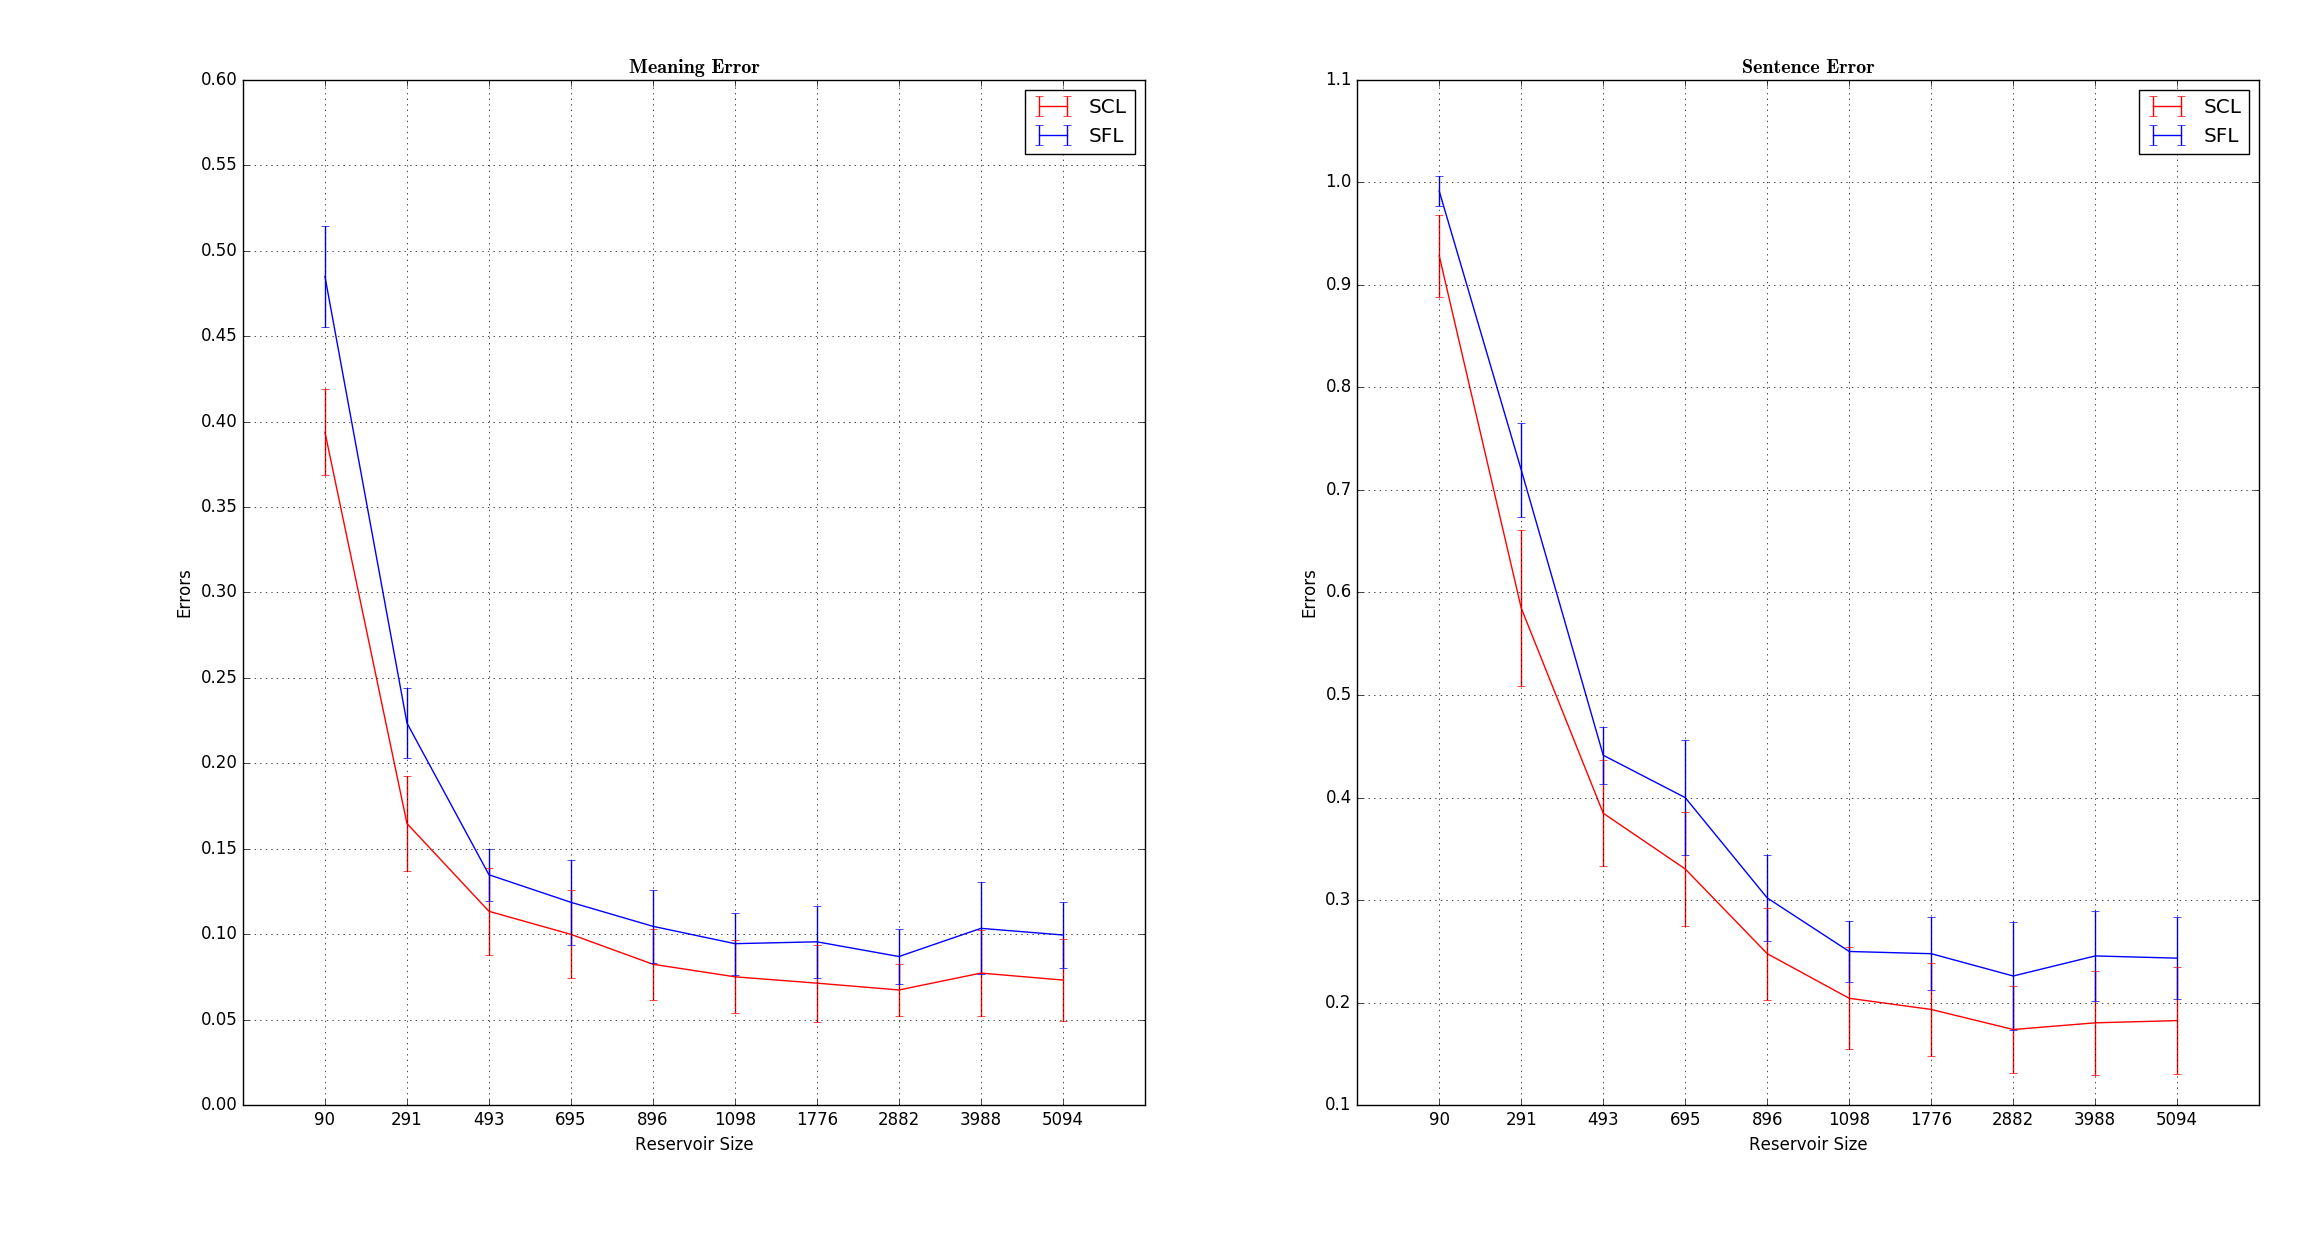
\includegraphics[width=1.0\linewidth]{reservoir_size_1}
\caption{\textbf{Effect of reservoir size on cross validation errors on Model Variant-1:} Description goes here.}
\label{fig:reservoir_size_1}
\end{figure}

We also studied the effect of reservoir size on the performance of model variant-2 when using word2vec word embeddings and also when using grammatical construction of sentence along with localist word representation. In figure \ref{fig:reservoir_size_2}, it can be clearly observed that the model variant-2 performs much better with word2vec word embeddings with all reservoir size when compared to use grammatical construction of sentence with localist word vector. Even the highest F1-Score ($F1 = 80.06 \%$) obtained using localist representation with reservoir size 2250 is much less than that of obtained using word2vec word embeddings with reservoir of size 200 (F1 = $ 93.56\%$). Overall with increase in reservoir size the classification score also increases irrespective of the word vectors used as an input to the model. The model also asymptotes when reservoir size is 200 and 600 with word2vec and localist vectors respectively, indicating that model can not be genralized further on this corpus (i.e. corpus-462). 

\begin{figure}[hbtp]
\centering
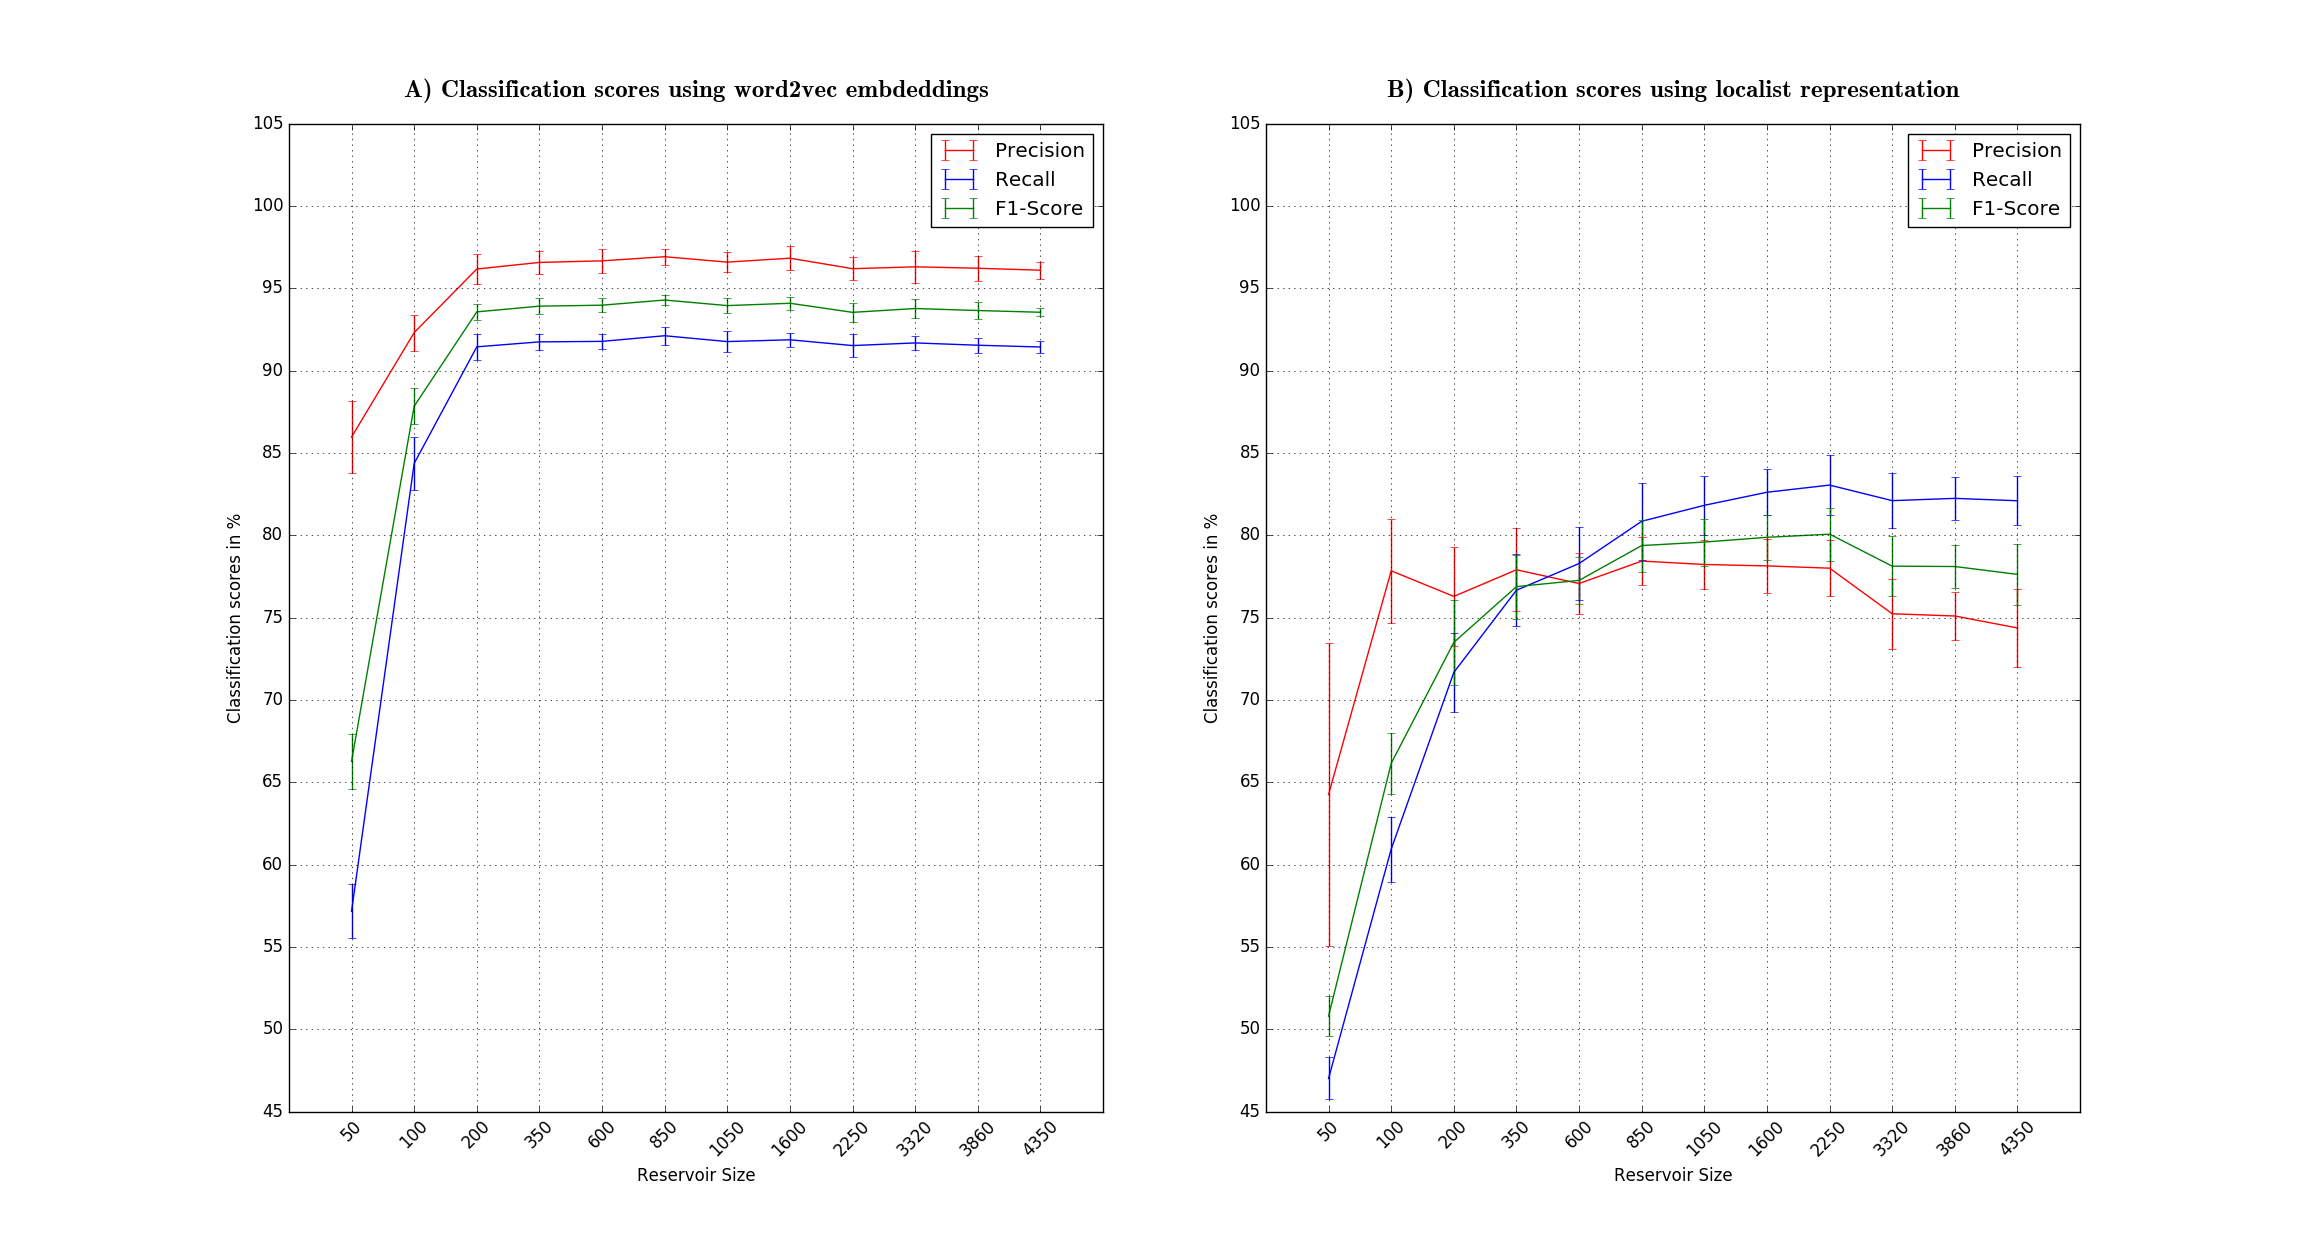
\includegraphics[width=1.0\linewidth]{reservoir_size_2}
\caption{\textbf{Effect of reservoir size on classification scores of Model Varinat-2:} Description goes here.}
\label{fig:reservoir_size_2}
\end{figure}



%TODO: Write the effect of reservoir size on the model variant-2

\subsection{Experiment-5: Effect of Corpus size}

In the previous experiments we noticed that the errors rates with Word2Vec-ESN model and classification scores model variant [] improved as we extended the corpus size from 45 to 462 sentences. To investigate the effect of corpus size and scaling capability of the model, we used extended corpus-90582(see section) for this experiment. As the corpus also contains $12\%$ of ambiguous sentences which impede the learning and generalization of the model, this experiment will also validate the model's ability to process the abmbiguous sentences.

In order to study the generalization capabilty of the model with different corpus size,  6 sub-corpora were created by randomly sampling $6\%$, $12\%$, $25\%$, $50\%$, $75\%$, $100\%$ of sentences from the orginal corpora of 90582 sentences\cite{end-to-end}. Each of the sub-corpora was exposed to the model and 2-fold cross validation is performed where the model was trained on half the sub-corpora size and tested on remaining half. The second half used for testing was then used to train the model and then tested on the first half used for training previously.

Figure \ref{fig:corpus_size_1} shows the cross validation errors rates with respect to corpus size while using model variant-1. It can be observed that with increase in corpus size from $6 \%$  to $25 \%$, the meaning error sharply drops from some $12.23 \%$ to $3.92 \%$ in SCL mode and from $12.10\%$ to $4.88 \%$ in SFL mode. Similarly, the sentence error also decreases from $54.43 \%$ to $21.89 \%$ in SCL and from $55.22 \%$ to $26.17 \%$ in SFL mode. When the sub-corpora size is $50\%$, where the model was trained only on $25\%$ of corpora size, the model already generalized with $17.11 \%$ sentence error and $2.98 \%$ meaning error in SCL mode and  $22.32 \%$ sentence error and $4.13 \%$ meaning error in SFL mode. The more gradual slope from $50 \%$ to $100 \%$ sub-corpora size in both the learning modes for meaning and sentence error indicates the model has already generalized and further increase in corpus size won’t have much effect on cross validation error.
 

\begin{figure}[hbtp]
\centering
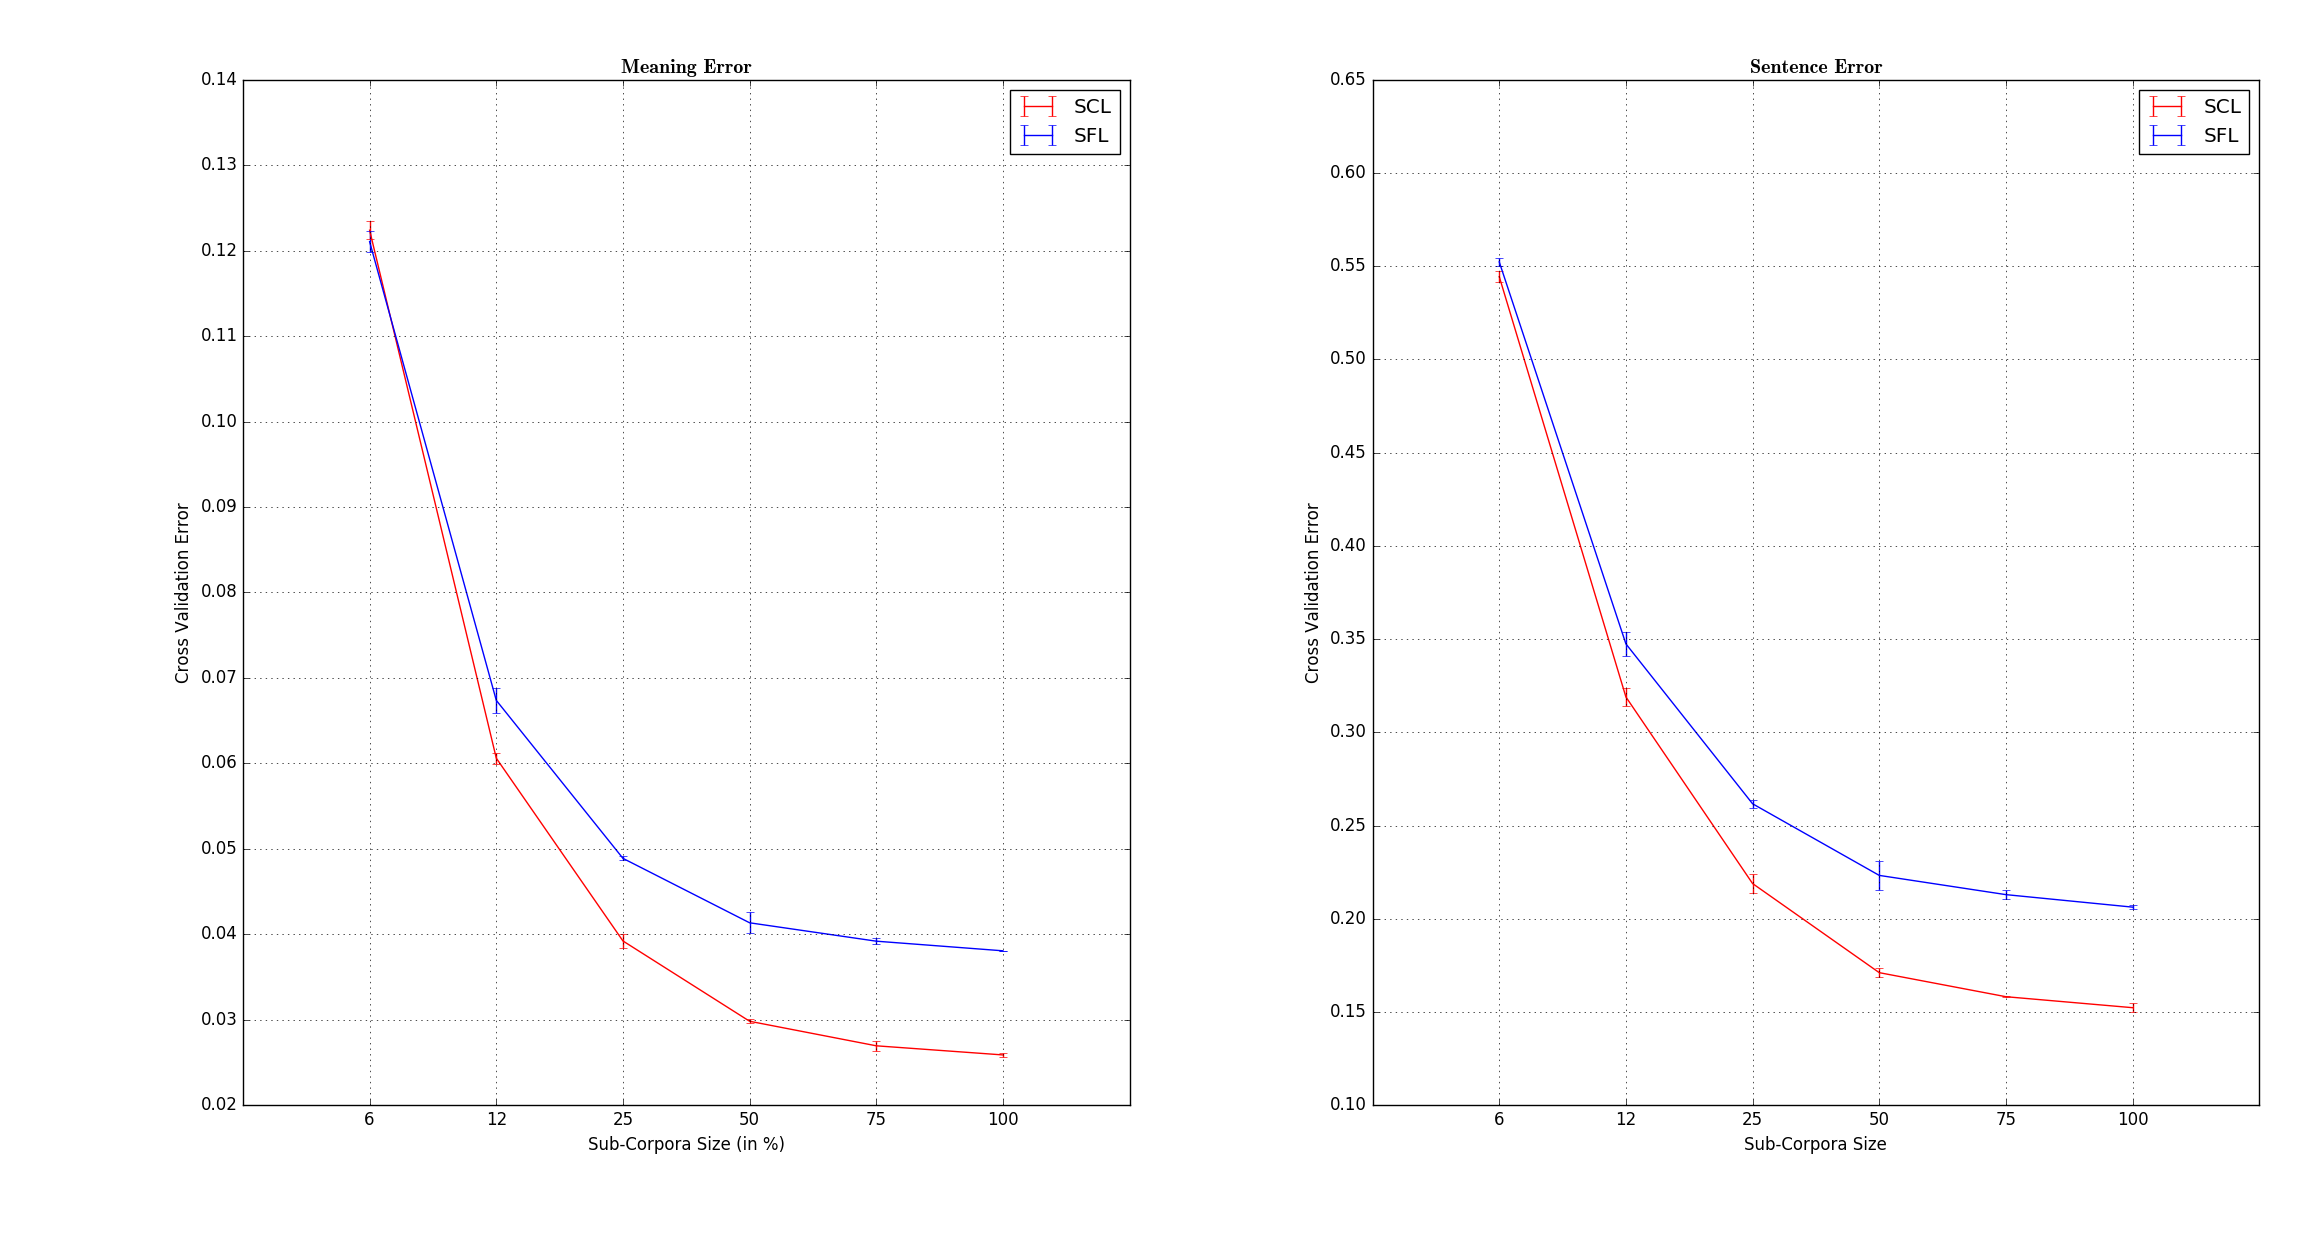
\includegraphics[width=1.0\linewidth]{corpus_size_1}
\caption{\textbf{Effect of corpus size on cross validation errors:} Description goes here.}
\label{fig:corpus_size_1}
\end{figure}


\begin{figure}[hbtp]
\centering
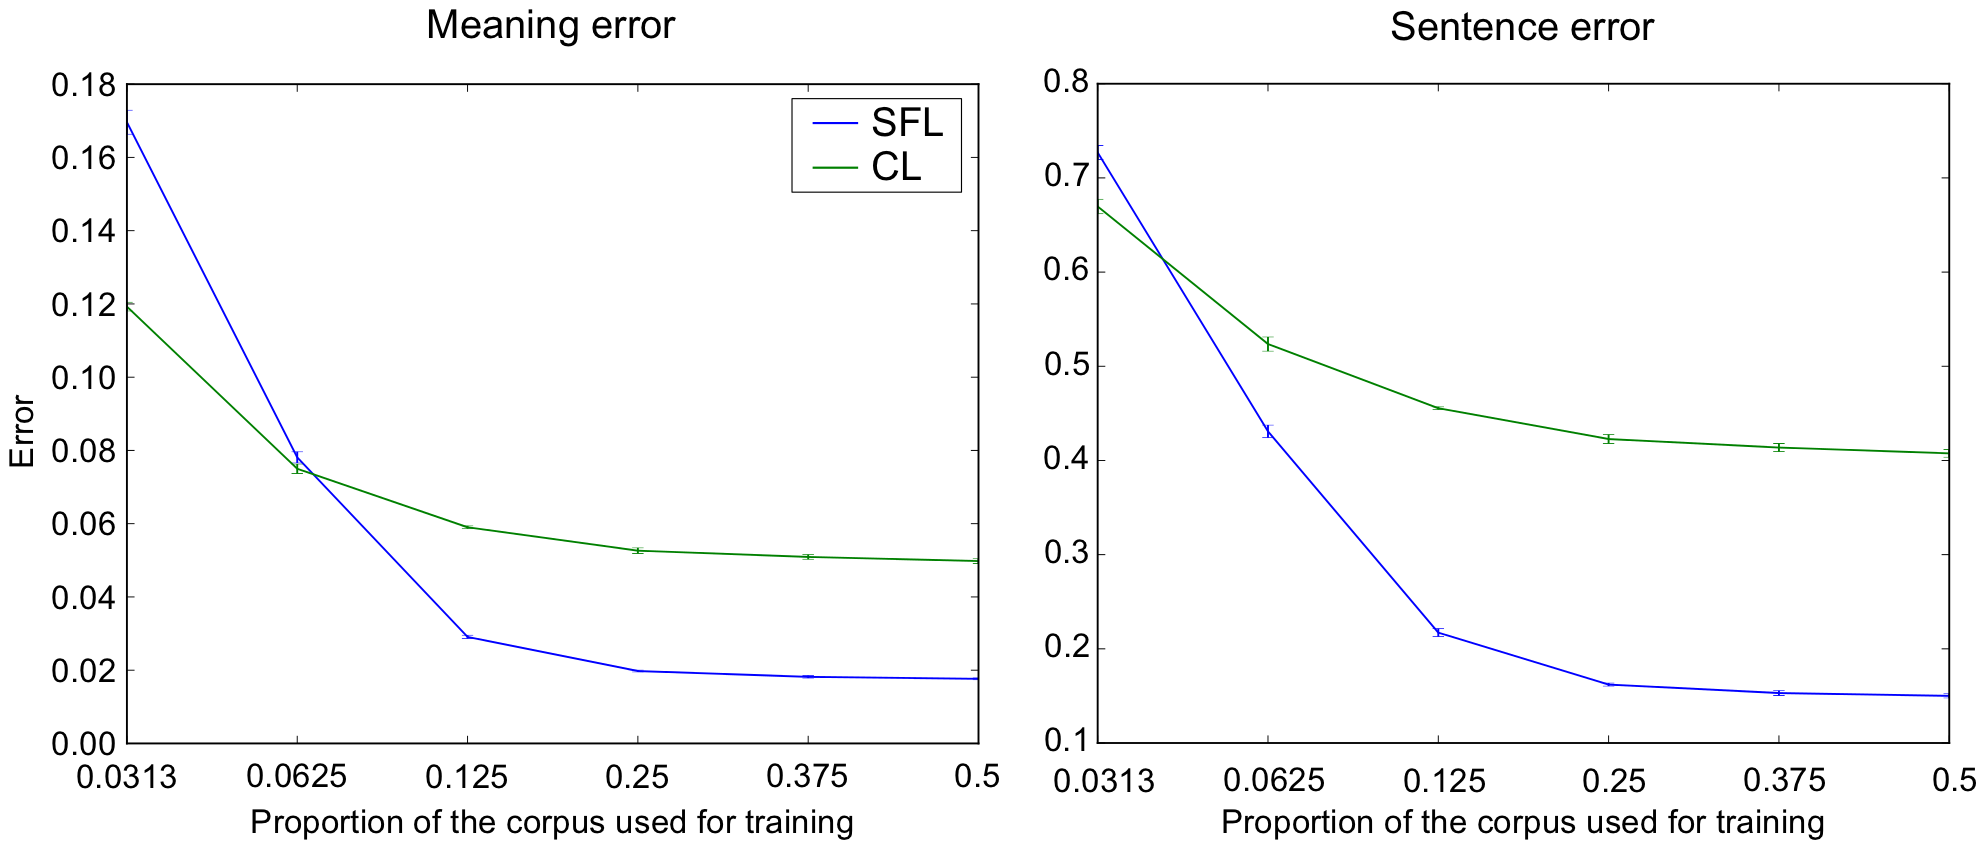
\includegraphics[width=1.0\linewidth]{corpus_size_xavier}
\caption{\textbf{Effect of corpus size on cross validation errors using localist word vector as reported in [ref?]:} Description goes here.}
\label{fig:corpus_size_xavier}
\end{figure}


\newpage

\subsection{Experiment-6: Neural output activity of the model}

In the previous experiments we observed that both the model variants generalized well and cross validation error rates dropped with increase in reservoir size. As we saw that model variants performs better when we increased corpus size from 45 sentences to 462 sentences. As corpus-45 contains sentence with uniques grammatical structure (i.e. active, passive, subject and object relative etc.) we added these 45 sentences to corpus-462 so the resultant corpus have 507 sentence (462+45) and analysed the activation produced by model variant-1 for the input sentences. We observed that while learning the model is re-analyzing the thematic roles across the time. The same behaviour was observed by xavier et. al [ref?] with sentences in grammatical constructions form and localist representation of words. However we observed that the model is making earlier predictions with word2vec embeddings. The reason for such a behavior is because the word2vec word embeddings were learned from the context words and each word vector encodes the information about neighbouring words. 

We examined and plotted the four sentences with active and passive constructions studied in Hinaur et al. [ref].

\begin{enumerate}[noitemsep]
\item the man gave the book to the boy. \label{eg-1:or-sent-17}
\item the man took the ball that hit the glass. \label{eg-1:or-sent-23}
\item the boy caught the ball that was thrown by the man.  \label{eg-1:or-sent-27} 
\item the ball was pushed by the man.  \label{eg-1:or-sent-16}
\end{enumerate}

Figure \ref{fig:act_analysis_1} shows the activations for these four different sentences across time. As all the four sentences start with "the", activation at this word is same for all the sentences. In sentences \ref{eg-1:or-sent-17} and \ref{eg-1:or-sent-23} with the arrival of first noun (i.e. man) the activation of noun-2 (i.e. book and ball) being an object of verb-1 is increased and confirmed with arrival of verb 'gave' and 'took' respectively.

\begin{figure}[hbtp]
\centering
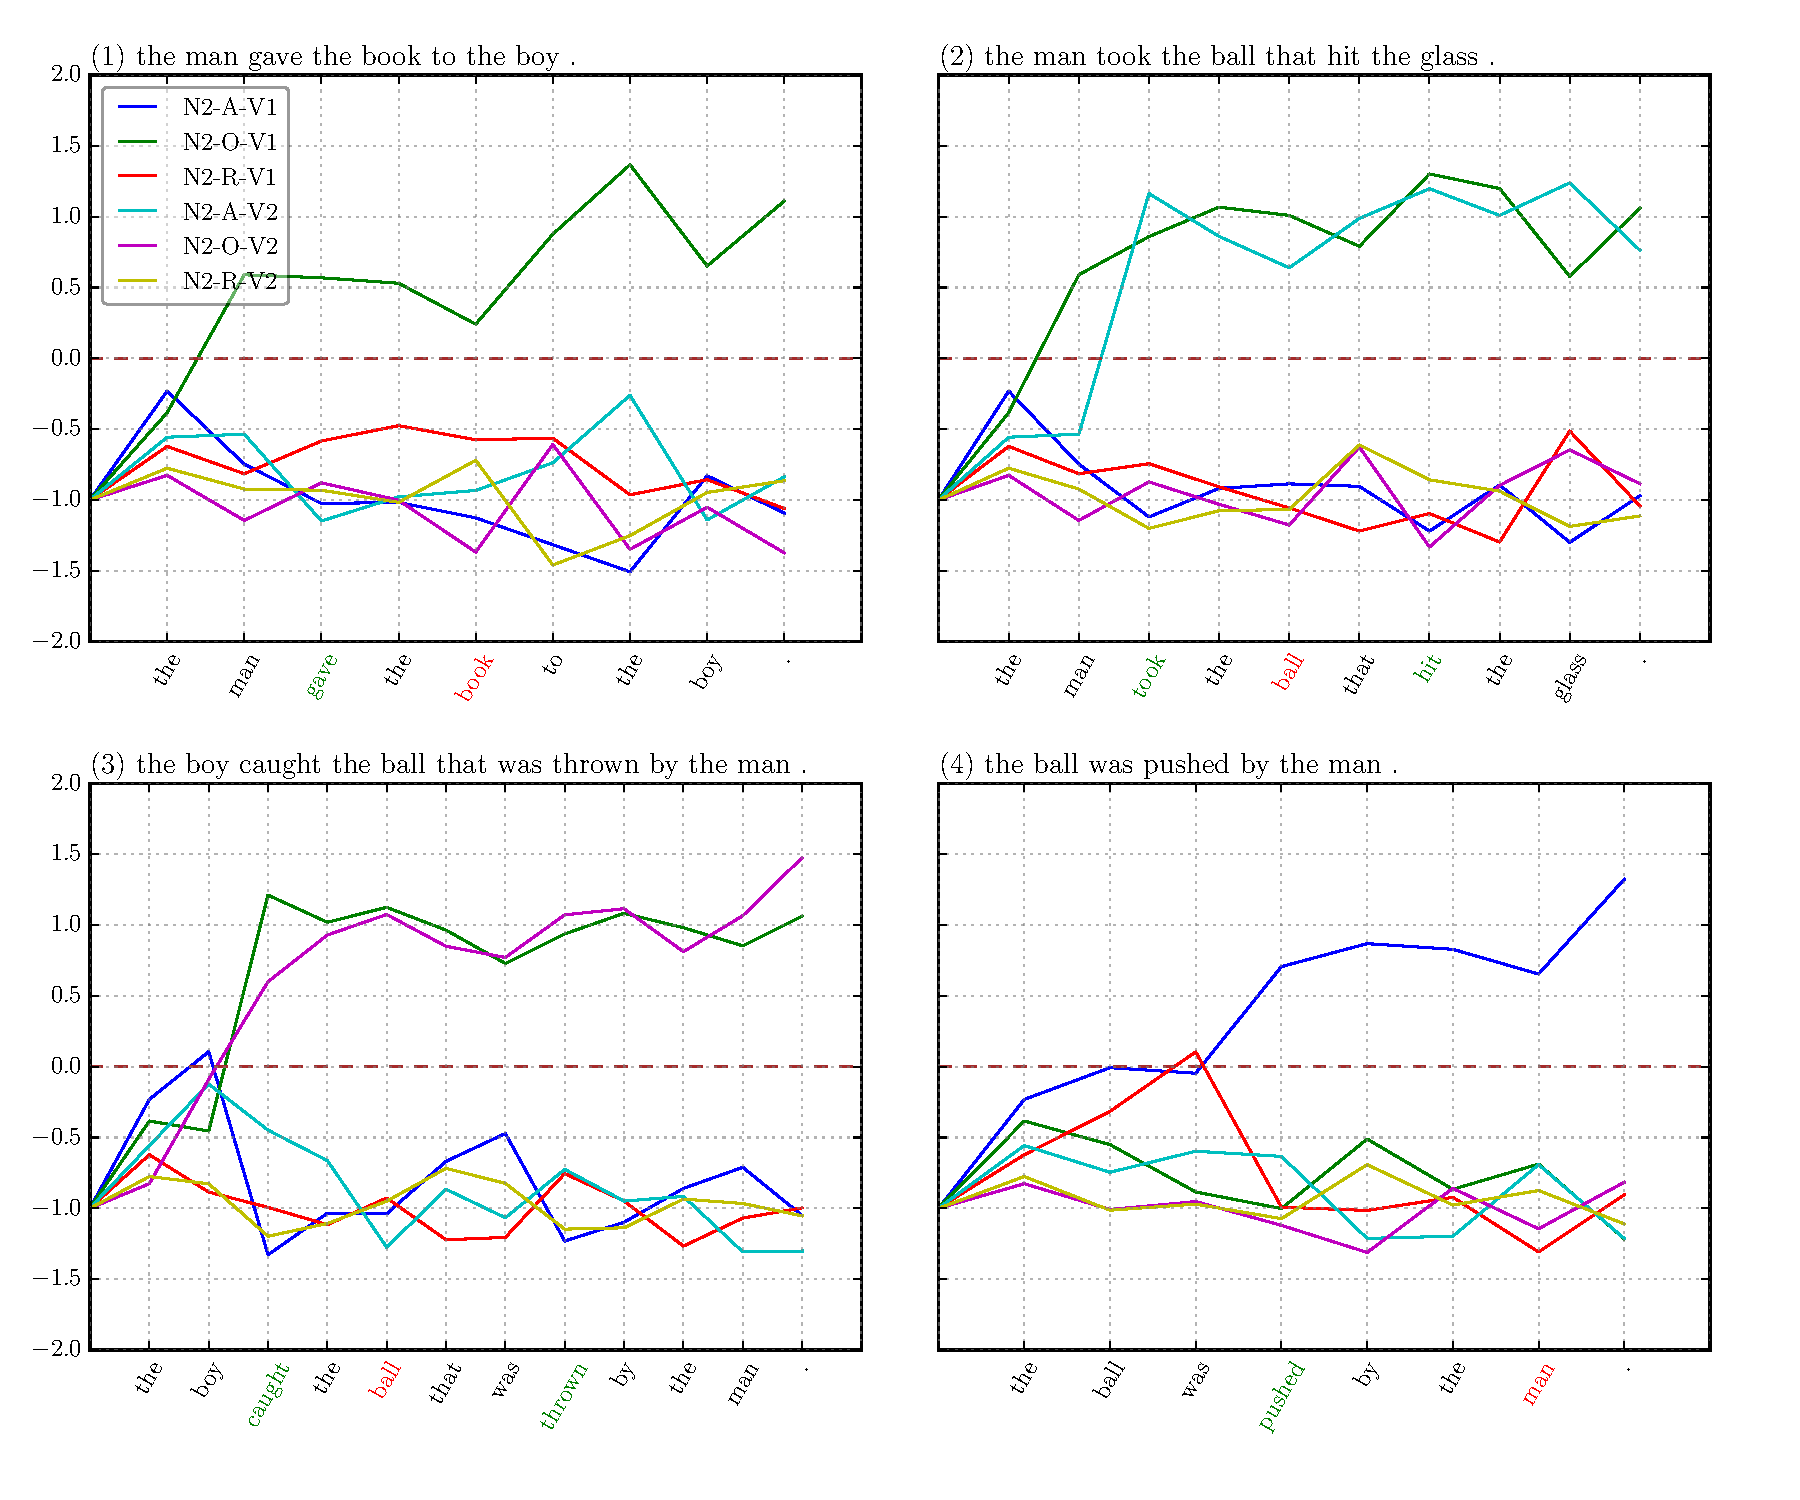
\includegraphics[width=1.0\linewidth]{act_analysis_1}
\caption{\textbf{Effect of corpus size on cross validation errors using localist word vector as reported in [ref?]:} Description goes here.}
\label{fig:act_analysis_1}
\end{figure}

Consider another two sentences 
\begin{enumerate}[noitemsep]
\item the dog that chased the cat ate the rat \label{eg-1:or-sent-17}
\item the cat that the dog chased bit the man. \label{eg-1:or-sent-23}
\end{enumerate}


\begin{figure}[hbtp]
\centering
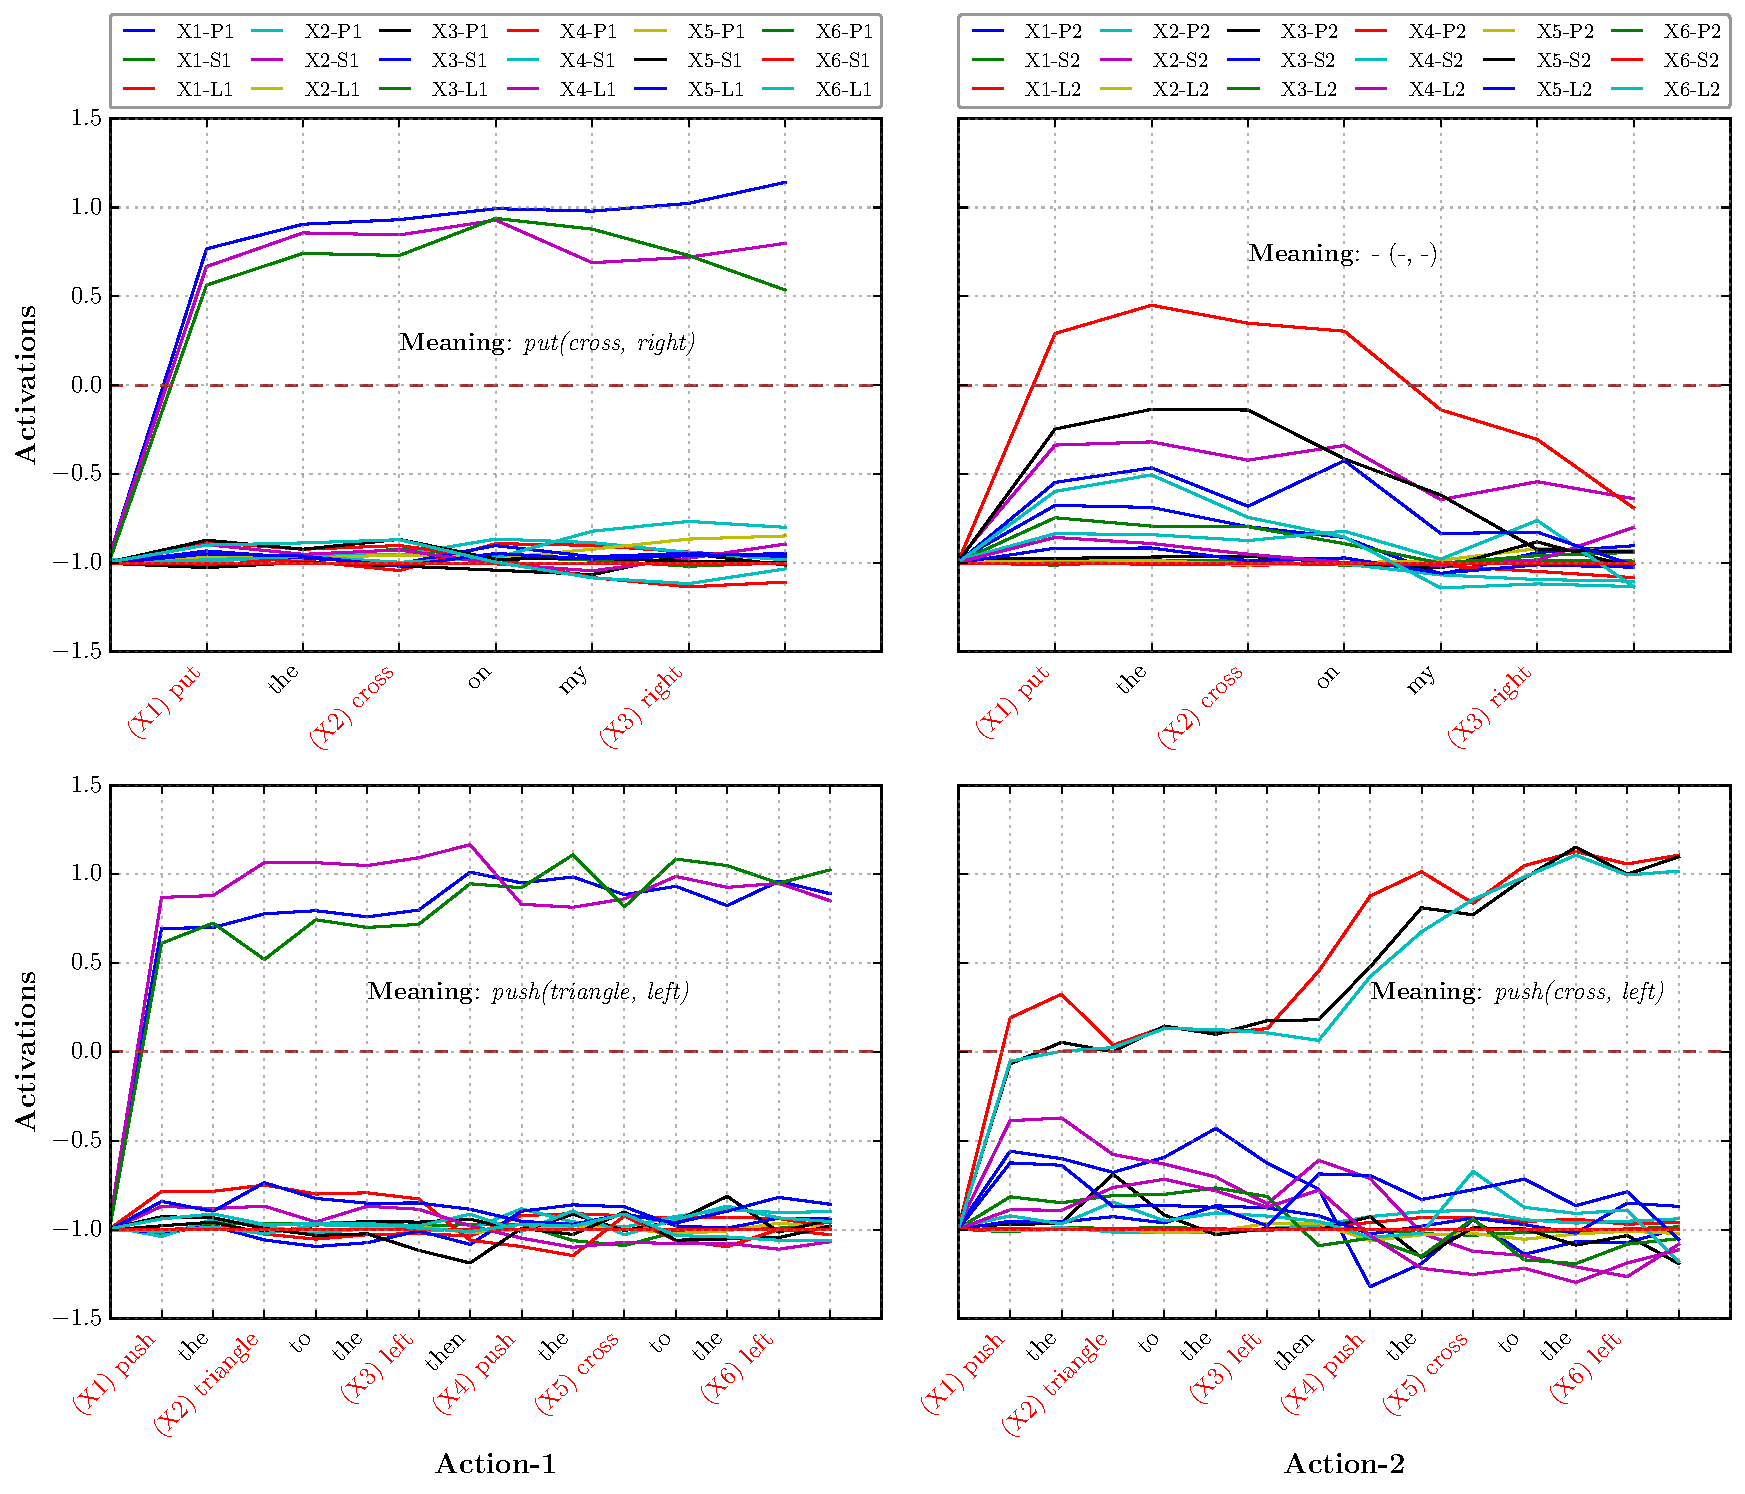
\includegraphics[width=1.0\linewidth]{act_analysis_2}
\caption{\textbf{Effect of corpus size on cross validation errors using localist word vector as reported in [ref?]:} Description goes here.}
\label{fig:act_analysis_2}
\end{figure}

\begin{figure}[hbtp]
\centering
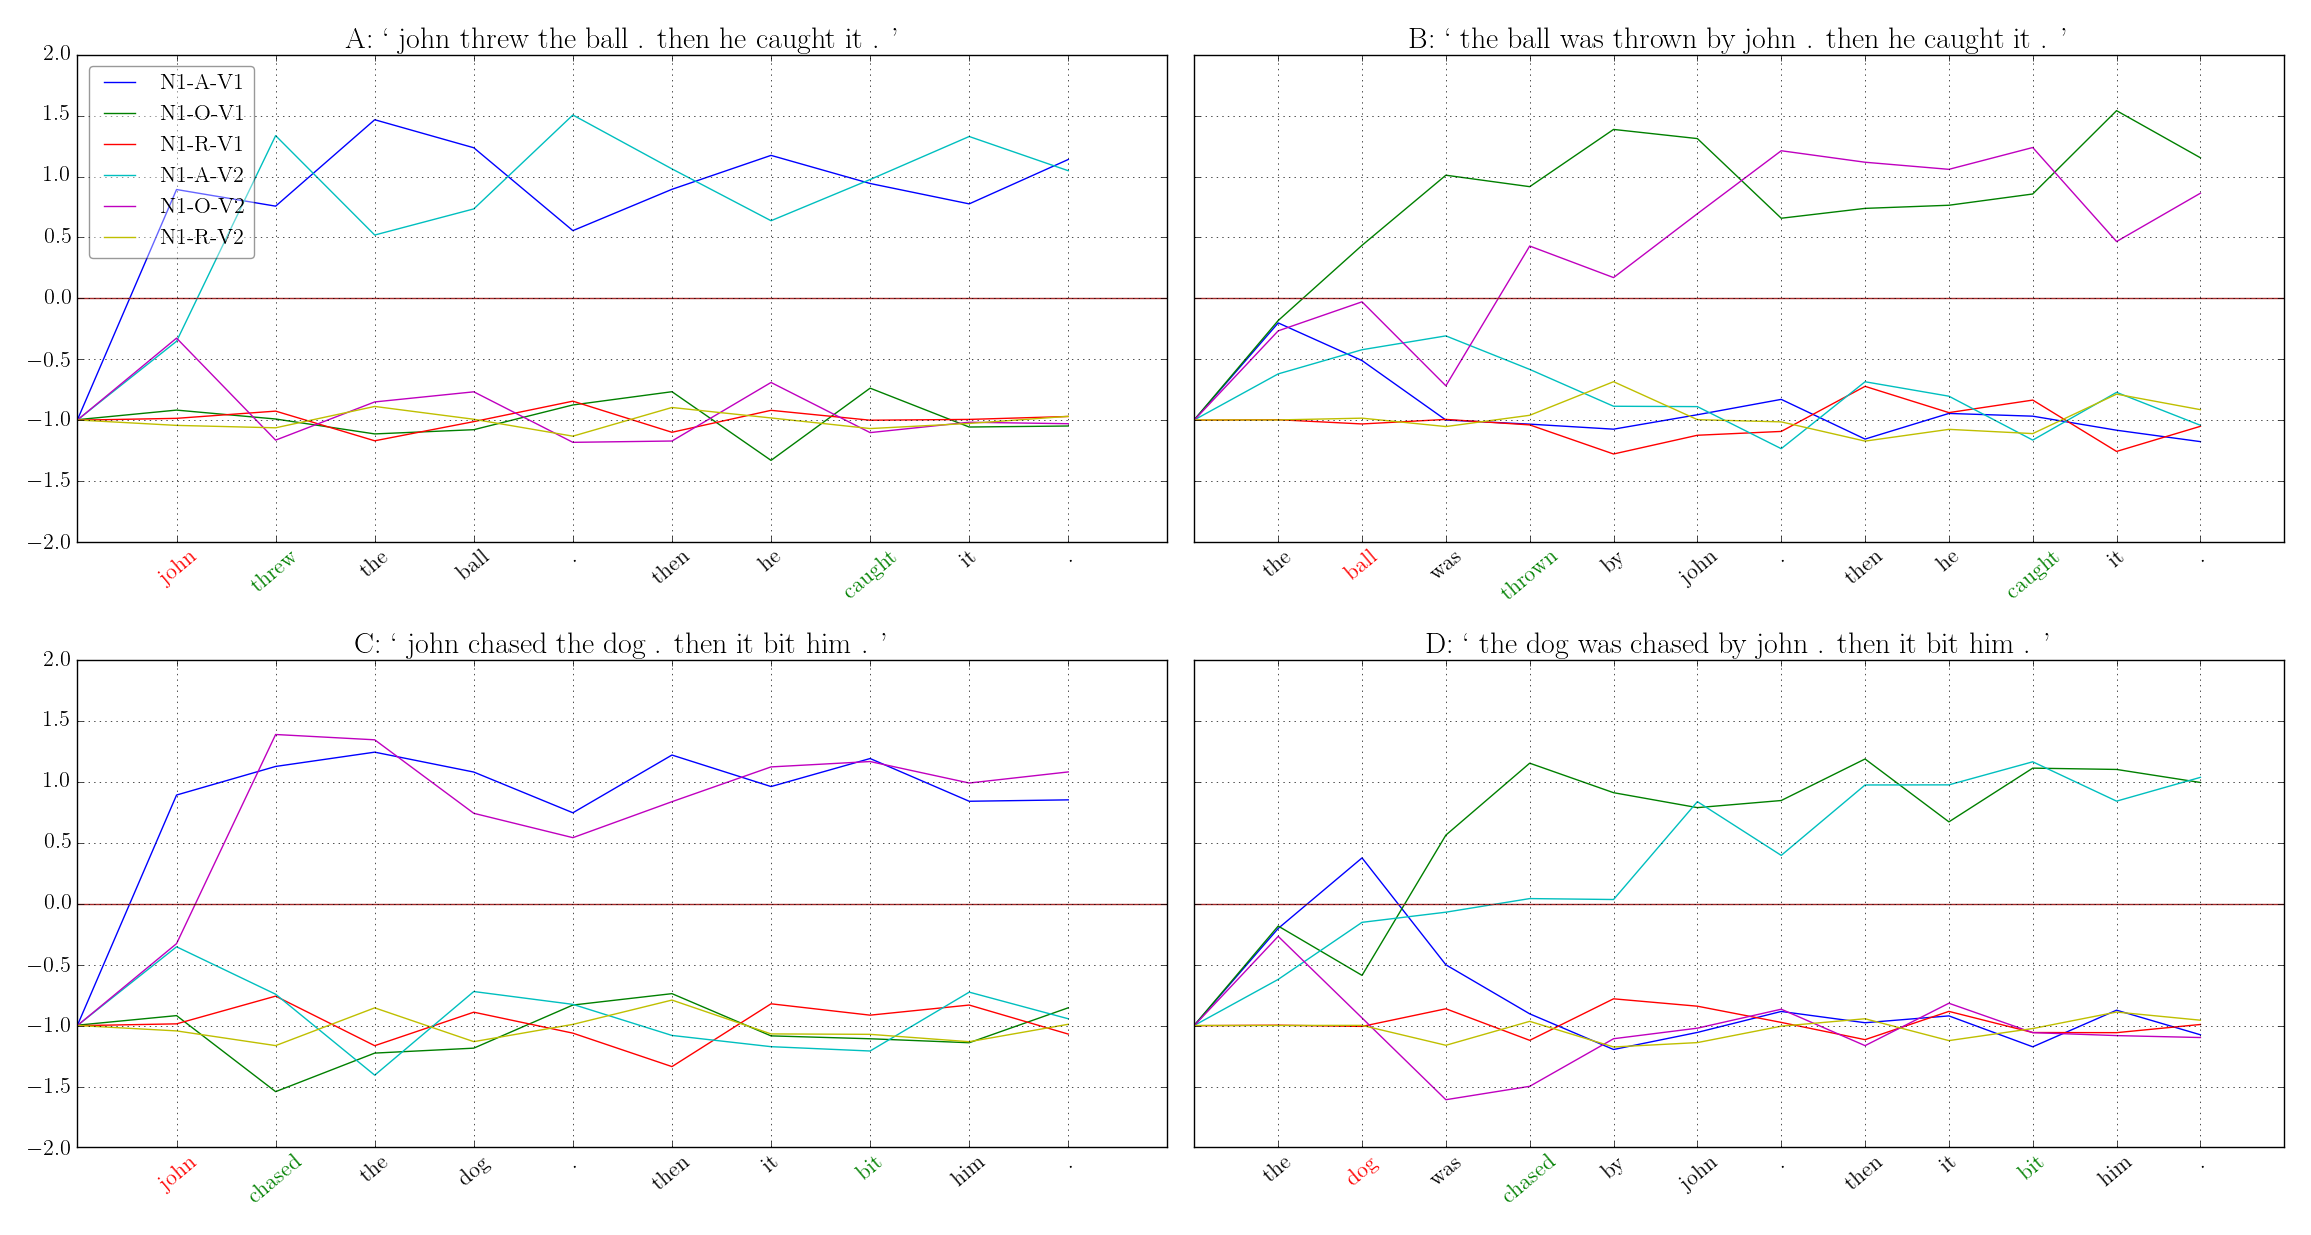
\includegraphics[width=1.0\linewidth]{act_analysis_3}
\caption{\textbf{Effect of corpus size on cross validation errors using localist word vector as reported in [ref?]:} Description goes here.}
\label{fig:act_analysis_3}
\end{figure}


\subsection{Experiment-7: Generalization on new corpus}

One may argue that the previously used corpus (corpus-462 and corpus-90k), which were artifically constructed using grammer is adding a bias to the model which makes it easier for the model to learn and genralize on these corpus. To answer this question, in this experiment we used the corpus collected by Hinaut et al. \cite{tra:tra:xavier_hri} in a Human Robot Interaction (HRI) study of language acquisition. The sentences in the corpus were collected from the real subjects interacting with the humanoid robot (iCub). The corpus contains 373 complex instruction to perform single or double actions with temporal correlation (see action performing task in Experiments of \cite{tra:tra:xavier_hri} for more details). For example, "Point to the guitar" is a one action command whereas "Before you put the guitar on the left put the trumpet on the right" is a complex instruction with double action, where second action is specified before the first action. Thus this data is complex enough to test the learnabilty and generalization of the model.  

To test the generalization of Word2Vec-ESN model on this corpus, leave-one-out (LoO) cross validation was performed. We chose LoO, so that results can be compared with that of obtained in $\theta RARes$ model of	Xavier et al.  \cite{tra:tra:xavier_hri}. As illustrated in table \ref{tab:corpus_373}, it can be observed that while using word2vec word embeddings over grammatical form and localist word vectors, of the input sentence, error improved by $26.31 \%$, $17.97 \%$ sentence error with 500 and 1000 reservoir neurons respectively. It can also be observed that with increase in reservoir size the sentence error also decreases. For this experiment we did not explore for the best parameters, but instead we used the optimized parameter obtained on corpus-462 in experiment 2 i.e. SR = 2.4, IS = 2.5 and LR = 0.07. This shows that previously learned model parameters are capably roboust enough to generalize on new corpus. 

\begin{table}
\centering
\begin{threeparttable}
\caption{Generalization error in sentence continuous learning mode for corpus-373.}
\label{tab:corpus_373}
\rowcolors{2}{gray!25}{white}
\begin{tabular}{llll}
\toprule
Reservoir 	 		& Sentence Error 	&  Word2Vec-ESN 		& $\theta RARes$ \\
\midrule                 
\textbf{500 N}		& mean(std.) 		& 42.65 ($\pm$ 1.36) 	& 68.96 ($\pm$ 2.03)  \\
					& Best 				& 26.54 				& 44.50  \\
\textbf{1000 N}		& mean(std.) 		& 40.29 ($\pm$ 1.13) 	& 58.26 ($\pm$ 1.37)\\
					& Best 				& 25.73 				& 34.85 \\
\bottomrule
\end{tabular}
\begin{tablenotes}
\small
\item 
Sentence errors (in $\%$) obtained with Word2Vec-ESN model and $\theta RARes$ in SCL mode for input sentences with reservoir of size 500 and 1000 neurons. The results reported are mean and standard deviation of 10 reservoir instances. The best error here means the count of sentence errors common in all 10 reservoir instances\cite{tra:xavier_hri}.  
\end{tablenotes}
\end{threeparttable}
\end{table}
\cleardoublepage

\chapter{Conclusion And Future Work}\label{conclusion}


\section{Conclusion}

To be written...

\section{Future Work}

For this work we currenly used the combination of word2vec model and ESN. The Echo state network has an advantage of modelling sequential data, thus the sequential and temporal aspect of a sentence is taken into account in this study for thematic role assignment. But the dependencies between thematic roles of sentences were not taken into account for learning. To model the conditional probality distrubtion of the thematic roles, Conditional Random Fields (CRF);a log-linear model; can be used \cite{crf:intro:sutton}. CRFs has been the one of the most successful apporach used earlier as well for classification and sequential data labelling tasks \cite{end-to-end, esn:esn_crf}. Thus the Word2Vec-ESN model, proposed in this study, can be used with an additional CRF unit at the end to model the temporal dependencies between the input sentences conditional on the corresponding themactic roles. Doing so allows the resulting model to capture concealed temporal dynamics present in the sentences\cite{esn:esn_crf}. 

Also several low dimensional word vector can be generated using the word2vec model. It was observed that with increase in word vector dimensions the accuracy on Semantic-Syntactic word relationship test set \cite{w2v:regularities_in_word_representations}  also increases till some point. However adding more dimensions results into reduced improvement \cite{w2v:mikolov_2013_efficient}. Although in the current study we used word a vector 50 dimension but the effect of other dimension were not explored. It would also be intersting to explore the effect of higher word vector dimension on the performance of Word2Vec-ESN model. Word2Vec word vectors obtained by training the model on one language corpus (say English) can also be translated to get the most similar word in any target language. This is achieved by linearly projecting the word vector of source languge on target language \cite{w2v:language_similarities}. Thus the Word2Vec-ESN language model can also be investigated for multiple language acquisition \cite{hinaut_multiple_lang}. 
\cleardoublepage

%%%%%%%%%%%%%%%%%%%%%%%%%%%%
% Appendices:
% these are optional! For most Bachelor-theses and some Master-thesis none of them is needed. 
% Just comment them if not needed.
\appendix
\fancyhead[LO,RE]{}                      % Define the header style for the appendixpages

\fancyhead[LE,RO]{\it Anhang A. Nomenclature}                %Adapt letter!
  \chapter{Complete Simulation Results}\label{app:completeResults}


%NOTE: 08/09/2016 results are copied after the simulation and are final, no need to change.
\begin{table}
\centering
\begin{threeparttable}
\caption{Effect of reservoir size on Word2Vec-$\theta$RARes model in different learning modes.}
\label{tab:corpus-size}
\rowcolors{2}{white}{gray!25}
\begin{tabularx}{\textwidth}{llYYYY}
  \toprule
  \hiderowcolors   
  &  & \multicolumn{4}{c}{Word2Vec-$\theta$RARes Model} \\
  \cmidrule(lr){3-6}   
  
Reservoir size  &  & \multicolumn{2}{c}{SCL mode} & \multicolumn{2}{c}{SFL mode} \\
  \cmidrule(lr){3-4} \cmidrule(lr){5-6}   
    
	   			& 			& ME 	& SE 		& ME 	 & SE 			\\
  \midrule
  \showrowcolors
  \textbf{90} 	& mean 		& 38.30 & 92.52  	& 46.41  & 98.09	 	\\
   			    & std 		& 1.53  & 1.67 		& 1.02   & 1.29 		\\
   			    		
  \textbf{291} 	& mean  	& 17.68 & 60.26 	& 22.00   & 69.13 		\\
				& std  		& 0.80 & 1.74 		& 0.97   & 3.03  		\\
  			   			
  \textbf{493} 	& mean 		& 11.63 & 40.34 	& 13.60   & 45.61 		\\
  				& std 		& 0.65 & 2.58 		& 0.64   & 2.14 		\\
  				 		
  \textbf{695}	& mean  	& 9.76 & 32.56 		& 10.64   & 34.83 		\\
  			  	& std 		& 0.61 & 1.56		& 0.58   & 1.42  		\\
					
  \textbf{896}	& mean  	& 8.39 & 25.56 		& 9.79   & 28.70 		\\
  			  	& std 		& 0.32 & 0.73		& 0.50   & 0.60  		\\
					
  \textbf{1098}	& mean  	& 7.98 & 22.17 		& 9.41   & 26.09 		\\
  			  	& std 		& 0.56 & 1.45		& 0.26   & 1.14  		\\
  			  		
  \textbf{1776}	& mean  	& 7.57 & 19.65 		& 9.79   & 24.70 		\\
  			  	& std 		& 0.39 & 0.84		& 0.43   & 0.90  		\\
  			  		
  \textbf{2882}	& mean  	& 6.99 & 18.04 		& 10.85   & 26.22 		\\
  			  	& std 		& 0.55 & 1.00		& 0.90   & 1.61  		\\
  			  		
  \textbf{3988}	& mean  	& 7.20 & 17.74 		& 11.02   & 26.17 		\\
  			  	& std 		& 0.48 & 0.45		& 0.50   & 1.63  		\\
  
  \textbf{5094}	& mean  	& 7.07 & 17.83 		& 11.06   & 25.87 		\\
  			  	& std 		& 0.53 & 1.54		& 1.08   & 1.34  		\\
  \bottomrule
\end{tabularx}
\begin{tablenotes}
\small
\item 
Meaning (ME) and Sentence error (SE) in different learning modes with Word2Vec-$\theta$RARes model. The errors are given in percentage and averaged over several model instances. The reservoir size is shown in first column. SCL: Sentence Continuous Learning; SFL: Sentence Final Learning; std: standard deviations. Simulations were performed with 5 model instances. Model was tested using 10-fold cross-validation approach.
\end{tablenotes}
\end{threeparttable}
\end{table}






%NOTE: 08/09/2016 results are copied after the simulation and are final, no need to change.
\begin{table}
\centering
\begin{threeparttable}
\caption{Effect of reservoir size on Word2Vec-ESN classifier in two different configurations.}
\label{tab:corpus-size}
\rowcolors{2}{white}{gray!25}
\begin{tabularx}{\textwidth}{llYYYYYY}
  \toprule
  \hiderowcolors   
  &  & \multicolumn{6}{c}{Word2Vec-ESN Classifier} \\
  \cmidrule(lr){3-8}   
  
Reservoir size  &  & \multicolumn{3}{c}{Configuration-1} & \multicolumn{3}{c}{Configuration-2} \\
  \cmidrule(lr){3-5} \cmidrule(lr){6-8}   
    
	   			& 			& Pr 	& Re 		& F1		& Pr 	 & Re 		& F1\\
  \midrule
  \showrowcolors
  \textbf{50} 	& mean 		& 83.09 & 52.59		& 61.12  	& 61.78  & 46.31	& 51.23 	\\
   			    & std 		& 4.57  & 7.76 		& 8.10		& 1.00   & 4.05 	& 3.11	\\
   			    		
  \textbf{100} 	& mean  	& 92.47 & 84.67		&88.05 		& 61.90  & 61.26 	& 60.72	\\
				& std  		& 1.14 	& 1.87		&1.37 		& 0.19   & 1.22  	& 0.58	\\
  			   			
  \textbf{250} 	& mean 		& 96.35 & 91.35 	&93.58		& 61.84  & 65.24 	& 62.51	\\
  				& std 		& 0.39 	& 0.25 		&0.18		& 0.10   & 0.84 	& 0.36	\\
  				 		
  \textbf{400}	& mean  	& 97.04 & 91.62		&94.03 		& 61.87  & 65.54 	& 62.67	\\
  			  	& std 		& 0.34 	& 0.24		&0.19		& 0.05   & 1.43  	& 0.62	\\
					
  \textbf{600}	& mean  	& 96.88 & 91.77		&94.05 		& 62.00  & 66.98 	& 63.21	\\
  			  	& std 		& 0.13 	& 0.13		&0.10		& 0.08   & 0.54  	& 0.24	\\
					
  \textbf{800}	& mean  	& 96.69 & 91.83		&94.00 		& 61.94  & 67.10 	& 63.30	\\
  			  	& std 		& 0.19 	& 0.07		&0.10		& 0.04   & 0.51  	& 0.26	\\
  			  		
  \textbf{1050}	& mean  	& 96.73 & 91.80		&94.01 		& 62.03  & 67.77 	& 63.54	\\
  			  	& std 		& 0.13 	& 0.03		&0.07		& 0.03   & 0.29  	& 0.17	\\
  			  		
  \textbf{1600}	& mean  	& 96.57 & 91.70		&93.88 		& 61.92  & 68.37 	& 63.85	\\
  			  	& std 		& 0.17 	& 0.10		&0.13		& 0.02   & 0.57  	& 0.23	\\
  			  		
  \textbf{2250}	& mean  	& 96.29 & 91.52 	&93.62		& 61.82  & 68.33 	& 63.82	\\
  			  	& std 		& 0.13 	& 0.05		&0.09		& 0.07   & 0.83  	& 0.37	\\
  
  \textbf{3320}	& mean  	& 96.05 & 91.38 	&93.46		& 61.80  & 68.24 	& 63.83	\\
  			  	& std 		& 0.22 	& 0.19		&0.21		& 0.08   & 0.94  	& 0.39	\\
  			  	
  \textbf{3860}	& mean  	& 96.07 & 91.39 	&93.47		& 61.85  & 67.74 	& 63.57	\\
  			  	& std 		& 0.22 	& 0.11		&0.15		& 0.05   & 2.80  	& 1.19	\\
  			  	
  \textbf{4500}	& mean  	& 95.91 & 91.28 	&93.34		& 61.89  & 70.01 	& 64.42	\\
  			  	& std 		& 0.25 	& 0.03		&0.13		& 0.07   & 3.60  	& 1.51	\\
  \bottomrule
\end{tabularx}
\begin{tablenotes}
\small
\item 
Precision (Pr), Recall (Re) and F1-Score (F1) in different configuration of Word2Vec-ESN classifier. The scores are given in percentage and averaged over several model instances. Configuration-1: raw sentences are processed, and distributed vectors of the argument-predicate pairs are input to ESN. Configuration-2: Sentences transformed to grammatical form and localist word vectors are input to ESN. std: standard deviations. Simulations were performed with 5 model instances. Model was tested using 10-fold cross-validation approach.
\end{tablenotes}
\end{threeparttable}
\end{table}


%NOTE: 08/09/2016 results are copied after the simulation and are final, no need to change.
\begin{table}
\centering
\begin{threeparttable}
\caption{Effect of sub-corpora size on Word2Vec-$\theta$RARes model in different learning modes.}
\label{tab:corpus-size}
\rowcolors{2}{white}{gray!25}
\begin{tabularx}{\textwidth}{llYYYY}
  \toprule
  \hiderowcolors   
  &  & \multicolumn{4}{c}{Word2Vec-$\theta$RARes Model} \\
  \cmidrule(lr){3-6}   
  
sub-corpora size  &  & \multicolumn{2}{c}{SCL mode} & \multicolumn{2}{c}{SFL mode} \\
  \cmidrule(lr){3-4} \cmidrule(lr){5-6}   
    
	   					& 		& ME 	& SE 		& ME 	 & SE 			\\
  \midrule
  \showrowcolors
  \textbf{5 $\%$} 	& mean 		& 12.18 & 54.84  	& 11.96  & 54.15	 	\\
   			    	& std 		& 0.19  & 0.52 		& 0.35   & 1.28 		\\
   			    		
  \textbf{12 $\%$} 	& mean  	& 6.13 & 32.63 		& 6.89   & 34.92 		\\
  			   		& std  		& 0.03 & 0.46 		& 0.18   & 0.78  		\\
  			   			
  \textbf{25 $\%$} 	& mean 		& 3.74 & 21.48 		& 4.91   & 26.10 		\\
  				 	& std 		& 0.04 & 0.42 		& 0.12   & 0.78 		\\
  				 		
  \textbf{50 $\%$}	& mean  	& 2.96 & 17.25 		& 4.17   & 22.41 		\\
  			  		& std 		& 0.04 & 0.39		& 0.11   & 0.57  		\\
					
  \textbf{75 $\%$}	& mean  	& 2.72 & 15.98 		& 3.95   & 21.33 		\\
  			  		& std 		& 0.03 & 0.30		& 0.11   & 0.64  		\\
					
  \textbf{100 $\%$}	& mean  	& 2.60 & 15.40 		& 3.84   & 20.78 		\\
  			  		& std 		& 0.02 & 0.25		& 0.09   & 0.57  		\\
  \bottomrule
\end{tabularx}
\begin{tablenotes}
\small
\item 
Meaning (ME) and Sentence error (SE) in different learning modes with Word2Vec-$\theta$RARes model. The errors are given in percentage. The sub-corpora (first column) is randomly sampled from corpus-90582. SCL: Sentence Continuous Learning; SFL: Sentence Final Learning; std: standard deviations. Simulations were performed with 5 model instances each having a reservoir of 1000 neurons. Model was tested using 10-fold cross-validation approach.
\end{tablenotes}
\end{threeparttable}
\end{table}




%NOTE: 08/09/2016 results are copied after the simulation and are final, no need to change.
\begin{table}
\centering
\begin{threeparttable}
\caption{Effect of word vector dimensions on Word2Vec-$\theta$RARes model in different learning modes.}
\label{tab:word-vector-size}
\rowcolors{2}{white}{gray!25}
\begin{tabularx}{\textwidth}{llYYYYYY}
  \toprule
  \hiderowcolors   
  &  & \multicolumn{6}{c}{Word2Vec-$\theta$RARes Model} \\
  \cmidrule(lr){3-8}   
  
  &  & \multicolumn{3}{c}{SCL mode} & \multicolumn{3}{c}{SFL mode} \\
  \cmidrule(lr){3-5} \cmidrule(lr){6-8}   
    
	   				& 			& ME 	& SE  	&	Best		& ME 	 & SE 		& Best		\\
  \midrule
  \showrowcolors
  \textbf{20} 		& mean 		& 14.68 & 40.46 & 	25.74		& 17.25  & 44.93 	& 29.49	 	\\
   			    	& std 		& 0.58  & 1.58 	&	-			& 0.76   & 1.36	 	& -			\\
   			    		
  \textbf{30} 		& mean  	& 14.23 & 39.87 &	26.01		& 16.61  & 43.46 	& 26.27 	\\
  			   		& std  		& 0.53 	& 0.57 	&	-			& 0.67   & 0.70  	& - 		\\
  			   			
  \textbf{50} 		& mean 		& 14.29 & 40.29 &	25.73		& 17.34  & 43.99 	& 26.54		\\
  				 	& std 		& 0.34 	& 1.13 	&	-			& 0.36   & 1.38 	& -		\\
  				 		
  \textbf{100}		& mean  	& 14.68 & 40.46 &	24.93		& 17.66  & 44.96 	& 30.02		\\
  			  		& std 		& 0.58 	& 1.58	&	-			& 0.55   & 1.66  	& -			\\
					
  \textbf{200}		& mean  	& 15.00 & 41.31 &	27.88		& 17.96  & 44.66 	& 29.49		\\
  			  		& std 		& 0.73 	& 1.55	&	-			& 0.63   & 1.19  	& -			\\
					
  \textbf{300}		& mean  	& 16.17 & 42.39	& 	31.36		& 19.19  & 46.51 	& 32.71		\\
  			  		& std 		& 0.75 	& 1.46	&	-			& 0.64   & 1.34  	& -	\\
  \bottomrule
\end{tabularx}
\begin{tablenotes}
\small
\item 
Meaning (ME), Sentence Error (SE) and Best value  for different word vector dimensions in different learning modes with Word2Vec-$\theta$RARes model. The errors are given in percentage. SCL: Sentence Continuous Learning; SFL: Sentence Final Learning; std: standard deviations. Simulations were done using corpus-373, with 10 model instances each having a reservoir of 1000 neurons. Model was tested using LoO cross-validation approach.
\end{tablenotes}
\end{threeparttable}
\end{table}
\cleardoublepage

\fancyhead[LE,RO]{\it Anhang B. Additional Proofs}            %Adapt letter!
  \chapter{Additional Proofs}\label{app:proofs}

\cleardoublepage

\fancyhead[LE,RO]{\it Anhang C. Complete Simulation Results}%Adapt letter!
  \chapter{Complete Simulation Results}\label{app:completeResults}
\cleardoublepage

% ... add as much appendices as you need (one can also add source code, for example)

%\fancyhead[LE]{\it \leftmark}
%\chapter{}
\fancyhead[LE,RO]{\it Bibliography}       % A bibliography never have a letter or numbering!
    \bibliographystyle{plain}             % Style for presenting the literature
    \addcontentsline{toc}{chapter}{Bibliography}% Add to the TOC
    \bibliography{thesis}
\cleardoublepage

%%%%%%%%%%%%%%%%%%%%%%%%%%%%
% Formal page 1
\vspace{2cm}
\chapter*{Erkl\"arung der Urheberschaft}
\label{sec:urheber}
\fancyhead[LE]{\it Erkl\"arung der Urheberschaft}
Ich versichere an Eides statt, dass ich die \trtype{} im Studiengang \trcourseofstudies{} selbstst\"andig verfasst und keine anderen als die angegebenen Hilfsmittel -- insbesondere keine im Quellenverzeichnis nicht benannten Internet-Quellen -- benutzt habe. Alle Stellen, die w\"ortlich oder sinngem\"a{\ss} aus Ver\"offentlichungen entnommen wurden, sind als solche kenntlich gemacht. Ich versichere weiterhin, dass ich die Arbeit vorher nicht in einem anderen Pr\"ufungsverfahren eingereicht habe und die eingereichte schriftliche Fassung der auf dem elektronischen Speichermedium entspricht.

%Ich versichere an Eides statt, dass ich die vorliegende \trtype{} selbstst\"andig und ohne unerlaubte Hilfe Dritter angefertigt habe. Alle Stellen, die inhaltlich oder w\"ortlich aus anderen Ver\"offentlichungen stammen, sind kenntlich gemacht. Diese Arbeit lag in gleicher oder \"ahnlicher Weise noch keiner Pr\"ufungsbeh\"orde vor und wurde bisher noch nicht ver\"offentlicht.

\vspace{4cm}
\noindent Ort, Datum \hfill Unterschrift

%The backcover is always empty
\newpage
\thispagestyle{empty}
\hspace{1cm}
\newpage

%%%%%%%%%%%%%%%%%%%%%%%%%%%%
% Formal page 2
\vspace{2cm}
\chapter*{Erkl\"arung zur Ver\"offentlichung}
\label{sec:urheber}
\fancyhead[LE]{\it Erkl\"arung zur Ver\"offentlichung}
Ich erkl\"are mein Einverst\"andnis mit der Einstellung dieser \trtype{} in den Bestand der Bibliothek.

\vspace{4cm}
\noindent Ort, Datum \hfill Unterschrift

%The backcover is always empty
\newpage
\thispagestyle{empty}
\hspace{1cm}
\newpage

\end{document}
%EOF

